\documentclass[pdftex,11pt,a4paper,oneside]{report}

% Set the margins with the geometry package
\usepackage[a4paper, left=4cm, right=4cm]{geometry}

\usepackage{amsmath}
\usepackage{algorithm}
\usepackage{algorithmic}
\usepackage{fancyhdr}
\usepackage{graphicx}
\usepackage{lipsum}
\usepackage{multirow}
\usepackage{setspace}
\usepackage{verbatim}
\usepackage{amsmath}
\usepackage{amsthm}
\usepackage{xcolor}
\usepackage[pagebackref=true,breaklinks=true,letterpaper=true,colorlinks,bookmarks=false]{hyperref}
\hypersetup{
    colorlinks = true,
    linkbordercolor = {white},
    citecolor = cyan
}
\usepackage{amssymb} % This package includes \mathbb

\newtheorem{definition}{Definition}

\fancyhf{}
\pagestyle{fancy}
\renewcommand{\headrulewidth}{0.2pt}

% Styles can be Sonny, Lenny, Glenn, Conny, Rejne, Bjarne and Bjornstrup
\usepackage[Sonny]{fncychap} 

\begin{document}

% !TEX root =  ../Dissertation.tex

\thispagestyle{empty}

\begin{spacing}{2}
	\begin{center}
		
\includegraphics[scale = 1.5]{Preamble/BirmCrest.png}
	\end{center}
	\vspace{10mm}
	\begin{center}
		\textbf{\Large Bisimulation Prioritized Experience Replay: Enhancing Online Reinforcement Learning through Bisimulation Behavioral-Based Priorities}
		\vspace{10mm}
	\end{center}
	\begin{center}
		\textbf{\large The Document Title}
		\vspace{20mm}
		\\\textbf{\Large Oscar Guarnizo}
		\vspace{20mm}
	\end{center}
	\begin{center}
		{\large School of Computer Science}
		\\ {\large College of Engineering and Physical Sciences}
		\\ {\large University of Birmingham}
		\\ {\large 2023-24}
	\end{center}
\end{spacing}

\pagenumbering{roman}



\chapter*{Abstract}
\addcontentsline{toc}{chapter}{Abstract}
%% !TEX root =  ../Dissertation.tex

\thispagestyle{empty}
\addcontentsline{toc}{chapter}{Dedication}

\begin{center}
	Dedicated to...
\end{center}

\newpage
 % Comment out for UG dissertations

\chapter*{Acknowledgements}
\addcontentsline{toc}{chapter}{Acknowledgements}
\textit{Foremost, I would like to express my sincere gratitude to my principal advisor, Dr. Mirco Giacobbe, and my co-advisor, Dr. Leonardo Stella, for their continuous support of my research, as well as their patience, responsibility, motivation, and enthusiasm.}

\textit{Equally important, I would like to thank Dr. Pablo Samuel Castro, the author of the MICo paper, for his invaluable advice and guidance, which helped me to better understand the topic. I truly appreciate your prompt responses to my questions and your enthusiasm in explaining your work to me. I hope to collaborate with you on future projects.}

\textit{I would also like to thank my friends and colleagues who offered ideas and comments about my project. In particular, I want to highlight the observations of Fernando Zhapa, Anthony Ramos, Jose Seraquive, and Joseph Gonzalez, which were instrumental in shaping this project.}

\begin{CJK}{UTF8}{bsmi}
\textit{A special thank you goes to my dear friend Yu Wen (黃郁雯), who accompanied me every day in the library throughout the entire journey of this thesis. Thank you for feeding me and cheering me up with your weird situations (like "losing a laptop"). Without a doubt, you made this thesis a more enjoyable and pleasant experience, and I am deeply grateful for your company.}
\end{CJK}

\textit{Last but not least, I would like to express my heartfelt thanks to my family, who always motivated and supported me throughout this master's journey. I am particularly grateful to my parents, Elizabeth and Vicente, for their constant calls and for taking the time to talk to me during both challenging and happy moments. I also thank my sisters, Evelyn and Ericka, for their frequent video calls filled with stories that lifted my spirits and kept me moving forward. Without their unwavering support, I would not have successfully completed this stage of my life.}
%% !TEX root =  ../Dissertation.tex

\chapter*{Declarations}
\addcontentsline{toc}{chapter}{Declarations}
 % Comment out for UG dissertations
%% !TEX root =  ../Dissertation.tex

\chapter*{Sponsorship and Grants}
\addcontentsline{toc}{chapter}{Sponsorship and Grants}

The research presented in this dissertation was made possible by the support of the following benefactors and sources:

\begin{itemize}

\item The Department of Computer Science, University of Warwick, Coventry, United Kingdom - Some Award (2004-2012)


\end{itemize} % Comment out for UG dissertations

\chapter*{Abbreviations}
\addcontentsline{toc}{chapter}{Abbreviations}

\begin{flushleft}

RL \hfill  Reinforcement Learning \\
BPER \hfill Bisimulation Prioritized Experience Replay \\
BPERcn \hfill Bisimulation Prioritized Experience Replay with strategy current-vs-next \\
BPERaa \hfill Bisimulation Prioritized Experience Replay with strategy all-vs-all \\
PER \hfill Prioritized Experience Replay \\
TD-error \hfill Temporal Difference Error \\
MICo \hfill Matching under Independent Couplings \\
ELP \hfill Expected Learning Progress \\
DQN \hfill Deep Q-Network \\
SAC \hfill Soft Actor-Critic
\end{flushleft}
%% !TEX root =  ../Dissertation.tex

\chapter*{Notations}
\addcontentsline{toc}{chapter}{Notations}

\begin{flushleft}

{\bf $r_2$} \hfill  Has some meaning

\end{flushleft}
 % Comment out for most dissertations 
% !TEX root =  ../Dissertation.tex

\tableofcontents

% !TEX root =  ../Dissertation.tex

\listoffigures
\addcontentsline{toc}{chapter}{List of Figures}

\listoftables
\addcontentsline{toc}{chapter}{List of Tables}

\newpage

% !TEX root =  ../Dissertation.tex

\pagenumbering{arabic}

\renewcommand{\chaptermark}[1]{\markboth{#1}{}}
\rhead{\small \thechapter . \leftmark}
\lfoot{\centering \thepage}


% !TEX root =  ../Dissertation.tex

\chapter{Chapter Title}


% !TEX root =  ../Dissertation.tex

\chapter{Background}
\label{sec:background}

\section{Reinforcement Learning}
\label{sec:reinforcement_learning}

% Reinforcement Learning (RL) \cite{sutton2018reinforcement} is an artificial intelligence learning paradigm, which, along with supervised and unsupervised learning, constitutes one of the three main approaches in machine learning. What distinguishes RL from other approaches is that the learning occurs through a trial-and-error process, where an \textbf{agent} receives \textbf{reward} signals (positive or negative) from an \textbf{environment}, leading to a focus on maximizing long-term positive rewards. The key elements, the agent and the environment, interact iteratively: the agent observes the state of the environment, takes an action accordingly, and receives a reward along with the next state from the environment (see Figure \ref{fig:rl_loop}). The primary goal of an RL agent is to maximize the cumulative reward, also known as the \textbf{return}. In this section, we will formally define these concepts.

Reinforcement Learning (RL) \cite{sutton2018reinforcement} is one of the three main paradigms in machine learning, alongside supervised and unsupervised learning. What distinguishes RL from other approaches is that the learning involves a trial-and-error process in which an \textbf{agent} interacts with an \textbf{environment} to maximize long-term rewards. The agent iteratively observes the current state of the environment, takes an action, and receives a \textbf{reward} signal (positive or negative), along with the next state (see Figure \ref{fig:rl_loop}). The primary objective of the RL agent is to maximize the cumulative reward, or \textbf{return}. In this section, we will formally define these concepts.

\begin{figure}[H]
    \centering
    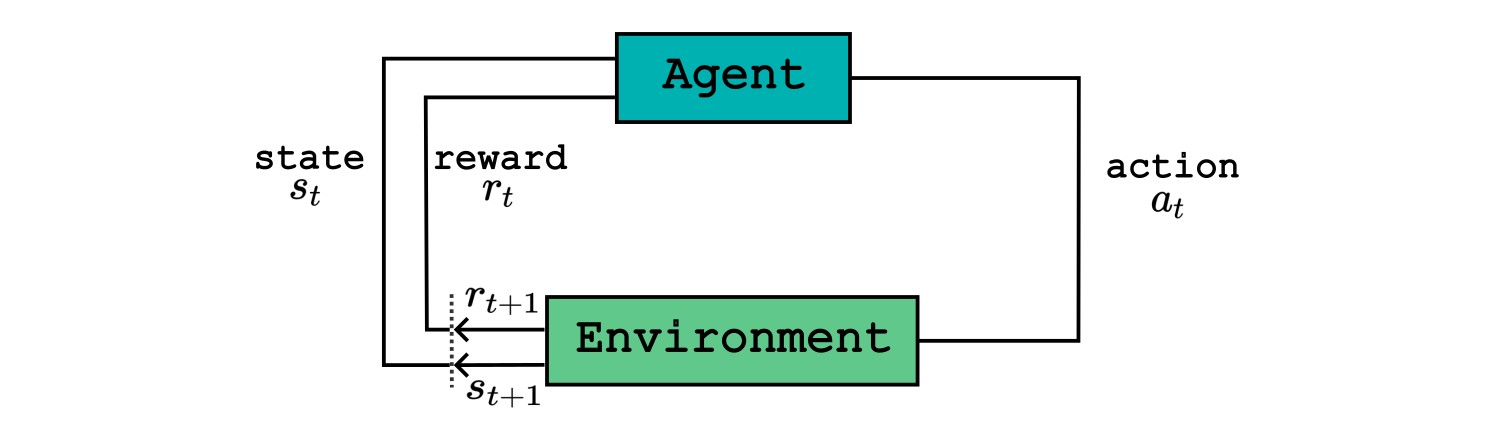
\includegraphics[width=1\linewidth]{Figures/rl_loop.jpg}
    \caption[Reinforcement Learning Loop]{\textbf{Reinforcement Learning Loop.} The agent iteratively interacts with the environment by taking action \(a_t\) based on state \(s_t\) and receiving reward \(r_t\) and next state \(s_{t+1}\).}
    \label{fig:rl_loop}
\end{figure}

% MDPs
\subsection{Markov Decision Process}
\label{sec:mdp_definition}

\textbf{Markov Decision Processes} (MDP) provide the formal framework upon which most RL algorithms are built. A \textbf{finite} MDP is an state transition system defined as a 5-tuple $M = \langle \mathcal{S}, \mathcal{A}, \mathcal{P}, \mathcal{R}, \gamma \rangle$, where 

\begin{itemize}
    \item $\mathcal{S}$ is a finite set of states,
    \item $\mathcal{A}$ is a finite set of actions,
    \item $P : \mathcal{S} \times \mathcal{A} \rightarrow \mathcal{P(S)}$ is a transition kernel, where $\mathcal{P(S)}$ is the set of probability distributions on $S$, and $P(s'|s, a)$ is the probability of transitioning from state $s$ to state $s'$,
    \item $\mathcal{R} : \mathcal{S} \times \mathcal{A}  \rightarrow \mathbb{R}$ is the reward function,
    \item and $\gamma \in [0, 1)$ is a discount factor.
\end{itemize}

For reference, a MDP can be visualized as a graph, as shown in Figure \ref{fig:mdp}, where the interaction between all components is illustrated. A MDP intuitively could be understood as the environment, while the agent decision-making mechanism is defined by a policy, which induces a Markov Chain on top of a MDP.

\begin{figure}[H]
    \centering
    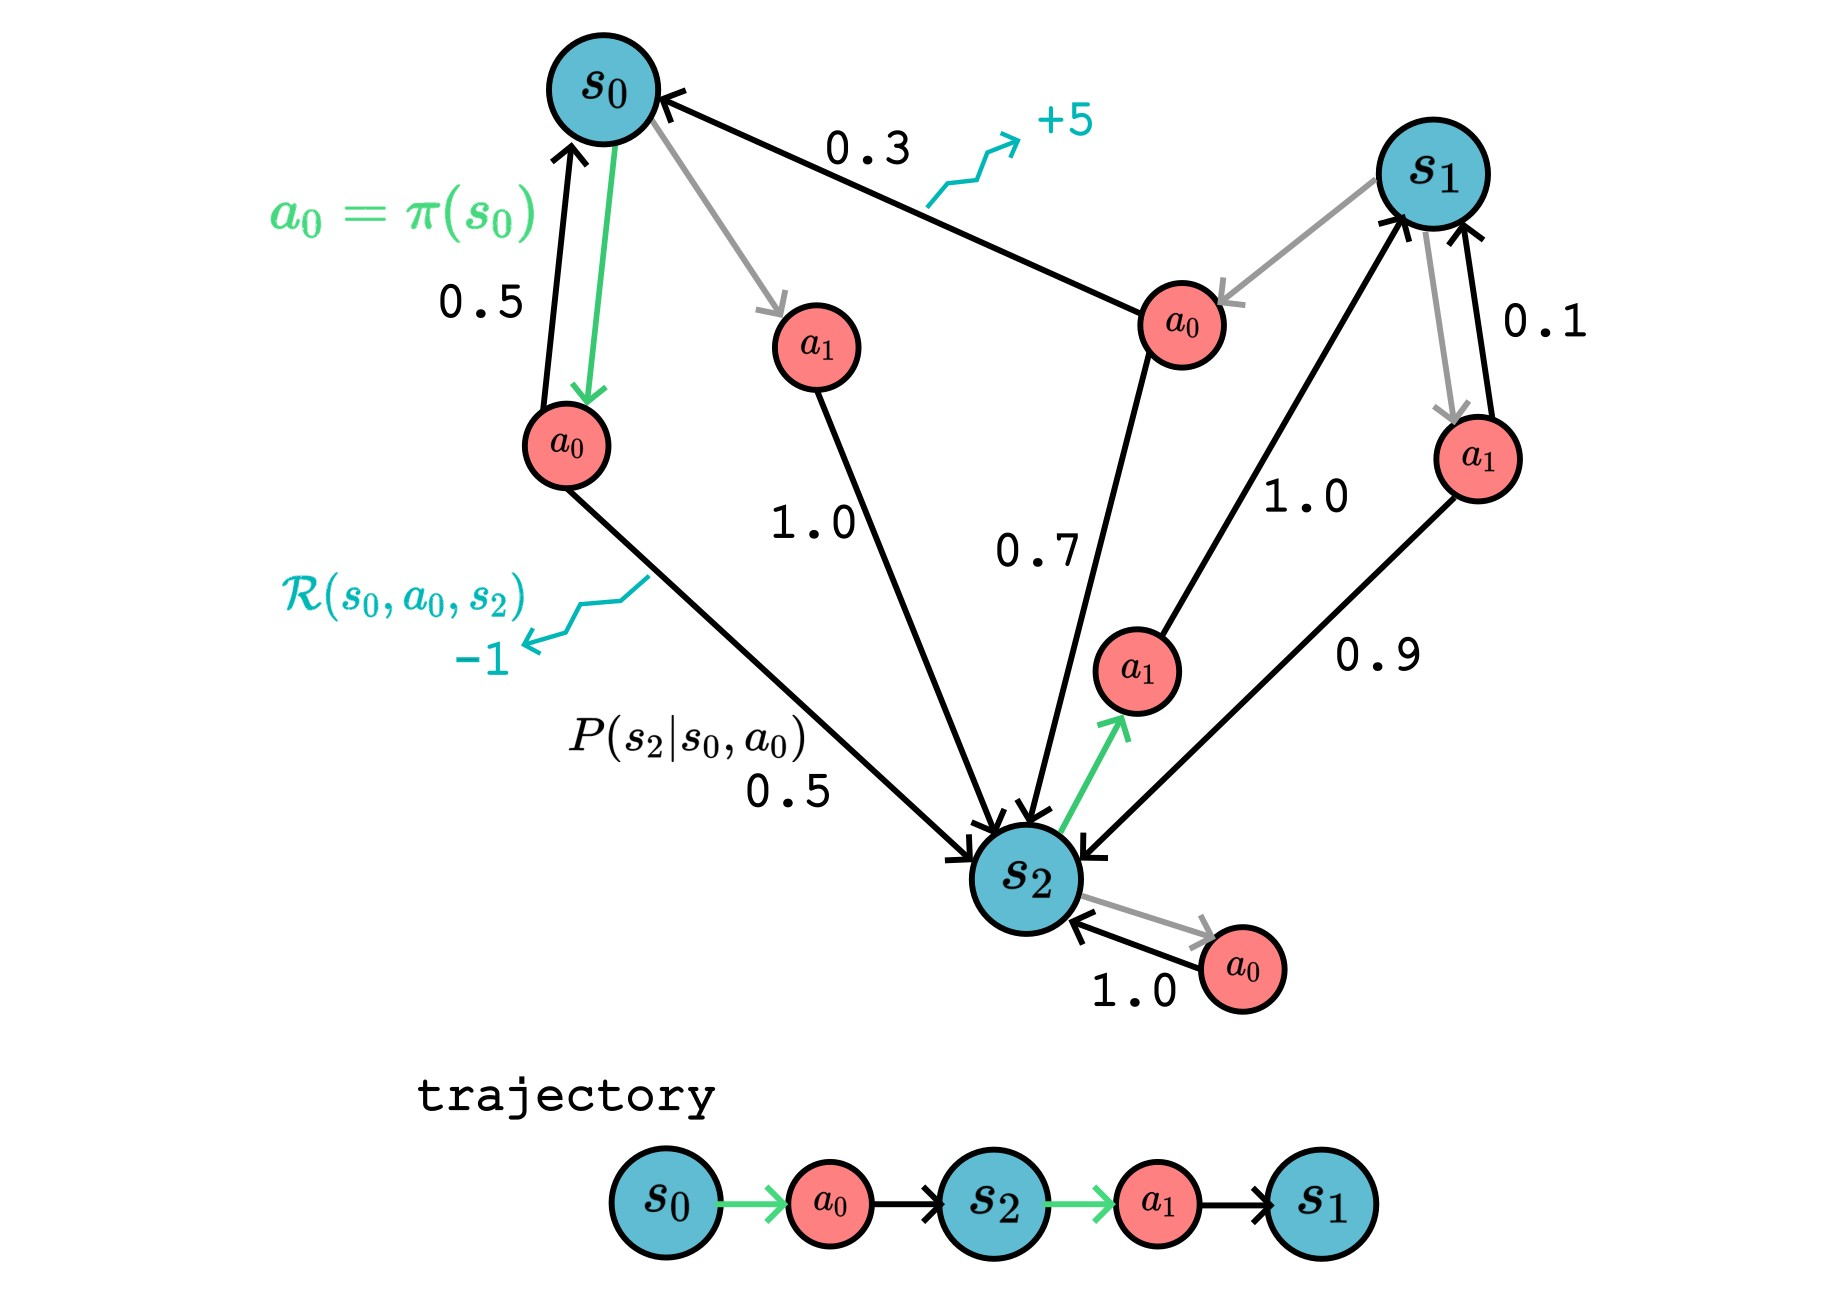
\includegraphics[width=0.95\linewidth]{Figures/mdp.jpg}
    \caption[Markov Decision Process]{\textbf{Markov Decision Process.} MDP elements: states, actions, rewards, and a policy determining decisions. The bottom part shows a trajectory generated by the current policy.}
    \label{fig:mdp}
\end{figure}


%Intuitively, the reinforcement learning (RL) loop depicted in Figure \ref{fig:rl_loop} can be understood as a trial-and-error process that induces an MDP. 

% For instance, if the states are represented by image frames from a simulator, the corresponding MDP would be described by \ref{}.

A \textbf{policy} $\pi \in \mathcal{P}(\mathcal{A})^\mathcal{S}$ describes the agent actions in a given state. A stochastic policy is a mapping from states to distributions over actions
\begin{equation}
    a_t \sim \pi(\cdot|s_t)
\end{equation}
, while a deterministic policy is a direct mapping from states to actions
\begin{equation}
a_t = \pi(s_t)    
\end{equation} 

\subsection{Trajectories, Return, and Value Functions}

The iterative interaction of an agent in the environment (see Figure \ref{fig:mdp}) is depicted in a \textbf{trajectory}\footnote{The trajectory, return and value functions explanations were based on \href{https://spinningup.openai.com/en/latest/spinningup/rl_intro.html}{OpenAI Spinning Up}} (also called rollout or \textbf{episode}), which is a sequence of states and actions.
$$\tau = (s_0, a_0, s_1, a_1, \dots )$$

where a \textbf{transition} is what happen between state $s_t$ and state $s_{t+1}$, in a deterministic transition as 
$$s_{t+1} = f(s_t, a_t)$$, 
or a stochastic transition $$s_{t+1} \sim P(\cdot | s_t, a_t)$$, where the action come from the policy.

The \textbf{reward} function $\mathcal{R}$ in the current work depends only on the current state and action taken, such that
$$r_t = \mathcal{R}(s_t,a_t)$$

The \textbf{return} $\mathcal{R}(\tau)$ is defined as the cumulative reward over a trajectory. It can be represented as a \textbf{finite-horizon undiscounted return}, which is the sum of rewards obtained within a fixed window of steps:
$$\mathcal{R}(\tau) = \sum_{t=0}^T r_t$$

, or as the \textbf{infinite-horizon discounted return}, which is the sum of all rewards ever obtained by the agent, but discounted by how far in the future they’re obtained. This formulation of return includes a discount factor $\gamma \in (0,1)$, which provide better theoretical convergence guarantees:

$$\mathcal{R}(\tau) = \sum_{t=0}^\infty \gamma^t r_t$$

In RL, any agent aims to obtain an optimal policy $\pi^\ast$ that maximizes the expected return when the agent acts according to it.

\begin{equation}
    \pi^\ast = \operatorname*{arg max}_\pi \mathop{\mathbb{E}}\limits_{\tau \sim \pi}\left[\mathcal{R}(\tau) \right]
\label{eq:rl_objective}
\end{equation}

To achieve this goal, in many cases such as with DQN (as we will discuss later), it is necessary to have a notion of the value of a state or state-action pair. The \textbf{value} is defined as the expected return when starting from that state or state-action pair and then following a particular policy indefinitely. Below are some key concepts related to \textbf{value functions} retrieved from \cite{SpinningUp2018}:

\begin{itemize}
    \item The \textbf{On-policy Value Function} gives the expected return if you start in state $s$ and always act according to policy $\pi$:
    \begin{equation}
    V^\pi(s) = \mathop{\mathbb E}_{\tau \sim \pi} \left[\mathcal{R}(\tau | s_0 = s)\right]
    \end{equation}
    \item The \textbf{On-Policy Action-Value Function}, $Q^{\pi}(s,a)$, which gives the expected return if you start in state $s$, take an arbitrary action $a$ (which may not have come from the policy), and then forever after act according to policy $\pi$:
    \begin{equation}
    Q^{\pi}(s,a) = \mathop{\mathbb E}_{\tau \sim \pi}\left[R(\tau)\left| s_0 = s, a_0 = a\right.\right]
    \end{equation}
    \item The \textbf{Optimal Value Function}, $V^*(s)$, which gives the expected return if you start in state $s$ and always act according to the optimal policy in the environment:
    \begin{equation}
    V^*(s) = \max_{\pi} \underE{\tau \sim \pi}{\mathcal{R}(\tau)\left| s_0 = s\right.}
    \end{equation}
    \item The \textbf{Optimal Action-Value Function}, $Q^*(s,a)$, which gives the expected return if you start in state s, take an arbitrary action a, and then forever after act according to the optimal policy in the environment:
    \begin{equation}
        Q^*(s,a) = \max_{\pi} \underE{\tau \sim \pi}{\mathcal{R}(\tau)\left| s_0 = s, a_0 = a\right.}
        \label{eq:q_optimal_value}
    \end{equation}


\end{itemize}

% \subsection{Value Iteration}
% \subsection{Q-Learning}



\subsection{Deep Q-Learning (DQN)}
\label{sec:dqn}
The Deep Q-Learning (DQN) \cite{mnih2013playing, mnih2015human} algorithm introduced a novel approach to train Q-learning algorithms using neural networks in high-dimensional, partially observable state spaces (e.g., raw pixels). It effectively addresses two important challenges in training deep neural networks for RL, such as highly-correlated states and non-stationary distribution issues.  To address both issues, DQN introduced a experience replay mechanism, which facilitates breaking temporal data correlations, leading to approximate independent and identically distributed (iid) data distributions.

%The RL is by nature a temporal sequential process, which produces highly-correlated states, and additionally; the data distribution evolves as the algorithm learns new behaviors, which is called a non-stationary distribution. From a supervised learning perspective, they made complicated the training because a supervised learning requires identical independent distributed data.

% NO image for experience replay (see Figure \ref{})
\textbf{Experience Replay} (ER) functions as a dataset with a \textbf{fixed capacity} $N$, storing tuples of experiences from the agent's interactions with the environment at different time steps during training, represented as
$$e_t = (s_t, a_t, r_t, s_{t+1}), \quad e_t \in \mathcal{E}$$

% In some scenarios, it is even possible to include a variable discount factor for each experience, such as $e_t = (s_t, a_t, r_t, \gamma_t, s_{t+1})$.

During training, mini-batches are randomly sampled from the experience replay to train a neural network $Q_\theta$, which is tasked with approximating the optimal state-action value function $Q^*$. In fact, DQN learning aims to estimate this optimal state-action value function, such that the optimal policy\footnote{Notice that by definition $Q^*(s,a)$ in Equation \ref{eq:q_optimal_value} represents the expected return for starting in state $s$, taking an arbitrary action $a$, and then following the optimal policy forever after. Therefore, by selecting the action with the maximum Q-value, we obtain the optimal policy that maximizes the expected return, same as the main RL goal in Equation \ref{eq:rl_objective}.} is

\begin{equation}
    \pi^*(s) = \arg \max_a Q^* (s,a)
    \label{eq:optinal_q_policy}
\end{equation}

To estimate the Q-value function, the DQN algorithm relies on a loss function derived from the Bellman equations \cite{sutton2018reinforcement}, which state that the value of a state is the reward you expect to receive from that state, plus the value of the subsequent state you transition to.
\begin{align*}
Q^*(s,a) &= \underE{s'\sim P(\cdot | s,a)}{r_t + \gamma \max_{a'} Q^*(s',a')}.
\end{align*}

As we aim to approximate $Q(s, a; \theta) \approx Q^*(s, a)$, a Q-network is trained to reduce the mean-square error in the Bellman equation by minimizing a sequence of loss function $L_i(\theta_i)$ that changes at each iteration $i$
\begin{align*}
    L_i (\theta_i) & = \underE{e_t \sim \mathcal{E}}{(y_i - Q(s_t, a_t; \theta_i))^2} \\
    & = \underE{(s_t, a_t, r_t, s_{t+1}) \sim \mathcal{E}}{(r_t + \gamma \max_{a'} Q(s_{t+1}, a'; \theta^-_{i}) - Q(s_t, a_t; \theta_i))^2} 
\end{align*}

where the optimal targets $r_t + \gamma \max_{a'} Q^*(s',a')$ are substituted with \textbf{approximated target values} for iteration $i$
\begin{equation}
    y_i = r_t + \gamma \max_{a'} Q(s_{t+1}, a'; \theta^-_{i})
\end{equation}

, and the gradients respect to the parameters $\theta_i$ are

\begin{equation}
    \nabla_{\theta_i} L(\theta_i) = \underE{(s_t, a_t, r_t, s_{t+1}) \sim \mathcal{E}}{ \delta_t \nabla_{\theta_i}Q(s_t, a_t; \theta_i)} 
\end{equation}

where the \textbf{temporal difference error} (or td-error) for the $e_i$ experience tuple corresponds to
\begin{equation}
    \delta_i = r_t + \gamma \max_{a'} Q(s_{t+1}, a'; \theta^-_{i}) - Q(s_t, a_t; \theta_i)
\end{equation}

Several important considerations should be taken into account when using this loss function in practice.

\begin{itemize}
    \item The parameters $\theta^-_{i}$ corresponds to a separated copy of the q-network parameters that is updated with $\theta_{i}$ every C gradient descent steps to stabilize the training.
    % \item Unlike supervised learning, the target depends on the parameters $\theta_{i-1}$, which change over time as the algorithm learns new behaviors.
    % \item The algorithm is \textit{model-free} because it does not require an explicit estimation of transitions distribution $P$ that govern the system.
    \item Although the algorithm approximates the greedy policy in Equation \ref{eq:optinal_q_policy}, it learns this strategy by using a behavioral \textbf{$\epsilon$-greedy policy}, which encourages exploration by taking a random action with probability $\epsilon$ during training 
    \begin{equation}
        \pi^\epsilon(a | s) = 
        \begin{cases} 
        a \sim \text{Uniform}(\mathcal{A}) & \text{with probability } \epsilon \\
        \arg\max_{a} Q(s, a; \theta) & \text{with probability } 1 - \epsilon
        \end{cases}
    \end{equation}
    
    Typically, this epsilon value is annealed over iterations to maintain a small value as learning approaches convergence.
    \item When learning from pixels, multiple frames $n$ are typically \textbf{stacked together} to represent a state in a preprocessing step. Additionally, the same action can be repeated over the $n$ stacked frames using a method called \textbf{skip frames} to reduce the training load. Thus, a state will be represented by $s_{t} = \phi(\{x_{t-n}, x_{t-(n-1)}, \cdots, x_{t}\})$, where the function $\phi$ stacks a window of $n$ frames (commonly $n=4$) while repeating the same action. For simplicity, we will refer to states in the algorithm and not the preprocessing function, but it is important to remind the reader that stacking and skip frames are used in a preprocessing step.
\end{itemize}

Algorithm \ref{algorithm:dqn} presents the pseudo-code for the DQN algorithm, modified slightly from the version in Mnih et al. \cite{mnih2013playing, mnih2015human} to run for a fixed total budget of $T$ (the total number of steps during the entire training), rather than running it per episode. This facilitates easier and fair comparisons with other extensions of the algorithm.

%Additionally, the algorithm show a per sample update procedure instead of the whole minibatch in order to make the comparison with prioritized alternatives clearlier, but the reader has to remember that in practice the gradients are calculated with vectorized procedures in the whole batch.



% \begin{algorithm}
% \caption{Deep Q-learning with Experience Replay (Mnih et al. \cite{mnih2013playing, mnih2015human})}
% \label{algorithm:dqn}
% \begin{algorithmic}[1]
% \State \textbf{Input:} minibatch $k$, step-size $\eta$, replay period $K$ and size $N$, budget $T$ (total steps).
% \State \textbf{Initialize} action-value function $Q$ with random weights $\theta$
% \State \textbf{Initialize} target action-value function $Q^-$ with weights $\theta^- = \theta$
% \State \textbf{Initialize} replay memory $\mathcal{D} = \emptyset$ with capacity $N$, $\Delta = 0$
% % \State Observe $s_0$ and choose $a_0 \sim \pi^\epsilon_\theta(s_0)$ 
% \For{$t = 1$ to $T$}
%     \State Observe $s_t$
%     \State Choose action $a_t \sim \pi^\epsilon_\theta(s_t)$
%     \State Execute action $a_t$ and observe $r_t$ and $s_{t+1}$
%     \State Store transition $(s_t, a_t, r_t, s_{t+1})$ in $\mathcal{D}$
%     \If{$t \equiv 0 \mod K$}
%         \For{$j = 1$ to $k$}
%             \State Sample transition $e_j \sim \text{Uniform}(\mathcal{D})$
%             \State Set $y_j = 
%             \begin{cases} 
%                 r_j & \text{for terminal } s_{j+1}\\
%                 r_j + \gamma \max_{a'} Q^-(s_{j+1}, a'; \theta^-) & \text{otherwise}
%             \end{cases}$
%             \State Compute TD-error $\delta_j = y_j - Q(s_j, a_j)$
%             \State Accumulate weight-change $\Delta \leftarrow \Delta + \delta_j \cdot \nabla_\theta Q(s_j, a_j)$
%         \EndFor
%         \State Update weights $\theta \leftarrow \theta + \eta \cdot \Delta$, reset $\Delta = 0$
%         \State Every C optimizing steps update $\theta^- \leftarrow \theta$
%     \EndIf
% \EndFor
% \end{algorithmic}
% \end{algorithm}

\begin{algorithm}[h]
\caption{Deep Q-learning with Experience Replay (Mnih et al. \cite{mnih2013playing, mnih2015human})}
\label{algorithm:dqn}
\begin{algorithmic}[1]
\State \textbf{Input:} minibatch $k$, step-size $\eta$, replay period $K$ and size $N$, budget $T$ (total steps).
\State \textbf{Initialize} action-value function $Q$ with random weights $\theta$
\State \textbf{Initialize} target action-value function $Q^-$ with weights $\theta^- = \theta$
\State \textbf{Initialize} replay memory $\mathcal{D} = \emptyset$ with capacity $N$ %$\Delta_{\{\xi, \omega\}} = 0$, $\Delta_\omega = 0$, $p_1 = 1$
% \State Observe $s_0$ and choose $a_0 \sim \pi^\epsilon_\theta(s_0)$ 
\For{$t = 1$ to $T$}
    \State Observe $s_t$
    \State Choose action $a_t \sim \pi^\epsilon_\theta(s_t)$
    \State Execute action $a_t$ and observe $r_t$ and $s_{t+1}$
    \State Store transition $(s_t, a_t, r_t, s_{t+1})$ in $\mathcal{D}$
        % \For{$j = 1$ to $k$}
        \State Sample minibatch $B \sim \text{Uniform}(\mathcal{D})$ of transitions $e_j$
        % \State Compute importance-sampling weight $w_j = \left( N \cdot P(j) \right)^{-\beta} / \max_i w_i$
        \State Set $y_j = 
        \begin{cases} 
            r_j & \text{for terminal } s_{j+1}\\
            r_j + \gamma \max_{a'} Q^-(s_{j+1}, a'; \theta^-) & \text{otherwise}
        \end{cases}$
        \State Compute TD-error $\delta_j = y_j - Q(s_{j}, a_{j}; \theta)$, and TD-loss $\mathcal{L}_{\text{TD}} = \delta_j^2 $
        \State Perform a gradient descent step on $\mathcal{L}_{\text{TD}}$
        % \State Update transition priority $p_j \leftarrow |\delta_j|$
        \State Every C optimizing steps update $\theta^- \leftarrow \theta$
\EndFor
\end{algorithmic}
\end{algorithm}

\subsection{Prioritized Experience Replay}
\label{sec:per}
Schaul et al. \cite{schaul2015prioritized} explored the limitations of the ER and discovered that a DQN algorithm revisits the same experience tuple an average of eight times, with not all revisits leading to significant improvements. As a result, they proposed Prioritized Experience Replay (PER), which non-uniformly samples experiences from the replay buffer based on a priority measure. While they left room for exploring other potential priority measures, they hypothesized that TD-error could serve as an indicator of expected learning progress. According to Schaul et al. \cite{schaul2015prioritized}, the \textbf{Expected Learning Progress} (ELP) is the idealised criterion to assign a priority value with the amount the RL agent can learn from a transition in its current state. By using TD-error as a priority measure, they aimed to more frequently replay experiences that are likely to result in those greater improvements.

Specifically, the sampling probability $P(i)$ of an experience tuple $e_i$ is defined as
\begin{equation}
    P(i) = \frac{p_i^\alpha}{\sum_k p_k^\alpha}
\end{equation}

where $\alpha$ controls the degree of prioritization, with $\alpha = 0$ the uniform case, and $p_i$ is the priority of an experience tuple $e_i$. Then, a \textbf{proportional prioritization}\footnote{An alternative \textbf{ranked-based prioritization}, defined as $p_i = \frac{1}{rank(i)}$, was also evaluated, where the $rank(i)$ represents the index of the experience in the buffer sorted according the TD-error $| \delta_i |$. This strategy employs a piece-wise linear function with $k$ segments to enhance sampling efficiency} assigns the priority as 
\begin{equation}
    p_i = | \delta_i | + \epsilon
\end{equation}

where $\epsilon$ is used to revised experiences even when td-error equal zero. This strategy uses a 'sum-tree' data structure to sample efficiently from a large experience buffer without depending on the buffer capacity $N$.

% \footnote{An additional \textbf{ranked-based prioritization} $p_i = \frac{1}{rank(i)}$ was evaluated, where the $rank(i)$ is the index of the experience in the buffer sorted according the TD-error $| \delta_i |$. This strategy utilizes a piece-wise linear function with $k$ segments of equal probability, allowing to sample a segment and then sampling uniformly from that segment.} 

The prioritized method, however, introduces a bias in the estimation of the Q-values. As the algorithm prioritize certain experiences over others, they will be sampled more frequently than what normally occur; skewing the distribution of experiences. This skewness does not correspond to the actual distribution of experiences encountered in the environment (the true distribution), leading to biased Q-value estimates. To address this issue, Schaul et al. \cite{schaul2015prioritized} introduced a \textbf{weighted Importance Sampling} \cite{mahmood2014weighted} to adjust the contribution of each sampled experience in the update step, compensating for the fact that some experiences were over-sampled (and therefore should be down-weighted) while others were under-sampled (and therefore should be up-weighted). The weight per experience is defined as
\begin{equation}
    w_i = \left(\frac{1}{N} \cdot \frac{1}{P(i)} \right)^\beta
\end{equation}

, where $N$ is the buffer capacity, and $\beta$ is an hyperparameter to adjust the importance sampling, which in practice is annealed from an initial value $\beta_0$ to $1$. Additionally, this weight is normalized by the maximal weight $\frac{1}{\max_k w_k}$ to stabilize the learning by reducing very large updates (only scaling downwards). Then, the weighted gradient is defined as
\begin{equation}
    \nabla_{\theta_i} L(\theta_i) = \underE{(s_t, a_t, r_t, s_{t+1}) \sim \mathcal{E}}{ w_i \delta_t \nabla_{\theta_i}Q(s_t, a_t; \theta_i)} 
\end{equation}

Algorithm \ref{algorithm:dqn_per} presents the pseudo-code for the DQN algorithm including the PER extension. It is important to note that, for practical reasons, priorities are updated only for the transitions in the current sampled mini-batch, as it would be computationally inefficient to update the entire replay buffer, especially when it is large. Additionally, new transitions added to the experience replay are assigned with a maximum priority to ensure that all experiences are sampled at least once.

% TODO:
% Domingo acabar background
% Lunes - Martes acabar State of the art
% Miercoles - Jueves - Viernes Metodologia
% Sabado Domingo Lunes Resultados y discusion
% Martes Miercoles Jueves Revision y mejorar graficas (5-7 acabado)
% 8 Ver si incluyo la prueba teorica
% Y aplicar a trabajos

\begin{algorithm}[h]
\caption{DQN with Prioritized Experience Replay (PER) (Schaul et al. \cite{schaul2015prioritized})}
\label{algorithm:dqn_per}
\begin{algorithmic}[1]
\State \textbf{Input:} minibatch $k$, step-size $\eta$, replay period $K$ and size $N$, exponents $\alpha$ and $\beta$, budget $T$ (total steps).
\State \textbf{Initialize} action-value function $Q$ with random weights $\theta$
\State \textbf{Initialize} target action-value function $Q^-$ with weights $\theta^- = \theta$
\State \textbf{Initialize} replay memory $\mathcal{D} = \emptyset$ with capacity $N$, $p_1 = 1$ (inital priority) %$\Delta_{\{\xi, \omega\}} = 0$, $\Delta_\omega = 0$, $p_1 = 1$
% \State Observe $s_0$ and choose $a_0 \sim \pi^\epsilon_\theta(s_0)$ 
\For{$t = 1$ to $T$}
    \State Observe $s_t$
    \State Choose action $a_t \sim \pi^\epsilon_\theta(s_t)$
    \State Execute action $a_t$ and observe $r_t$ and $s_{t+1}$
    \State Store transition $(s_t, a_t, r_t, s_{t+1})$ in $\mathcal{D}$ with maximal priority $p_t = \max_{i < t} p_i$
    \If{$t \equiv 0 \mod K$}
        % \For{$j = 1$ to $k$}
        \State Sample minibatch $B$ of transitions $e_j$ with probability $P(j) = \frac{p_j^\alpha}{\sum_i p_i^\alpha}$    
        \State Compute importance-sampling weight $w_j = \left( N \cdot P(j) \right)^{-\beta} / \max_i w_i$
        \State Set $y_j = 
        \begin{cases} 
            r_j & \text{for terminal } s_{j+1}\\
            r_j + \gamma \max_{a'} Q^-(s_{j+1}, a'; \theta^-) & \text{otherwise}
        \end{cases}$
        \State Compute TD-error $\delta_j = y_j - Q(s_{j}, a_{j}; \theta)$, and TD-loss $\mathcal{L}_{\text{TD}} = \delta_j^2 $
        \State Perform a gradient descent step on $\mathcal{L}_{\text{TD}}$, weighting the updates by $w_j$
        \State Update transition priority $p_j \leftarrow |\delta_j|$
        \State Every C optimizing steps update $\theta^- \leftarrow \theta$
    \EndIf
\EndFor
\end{algorithmic}
\end{algorithm}



\section{Bisimulation}
\label{sec:bisimulation_background}

Bisimulation, a concept of behavioral similarity, is central to this work. In the following sections, we will outline the key definitions of bisimulation that form the basis of our approach. For convenience, we reused the notation from \cite{castro2021mico} that is used interchangeable from now on. The next-state distribution for a given state-action pair $(s, a)$ is defined as,
$$P^a_s = P(\cdot|s, a) \in \mathcal{P(S)}$$, and the associated immediate reward 
$$r^a_s = r_t = \mathcal{R}(s,a)$$ 
Note not get confused with $P^a_s \neq P(s'|s, a)$, the former represents a distribution and the second one a probability value.

% \subsection{Preliminaries Concepts}

% \subsubsection{Equivalence Relation}

% \begin{definition}[Equivalence Relation]
% Let $X$ be a set. An equivalence relation on $X$ is a subset $R \subseteq X \times X$ that satisfies the following three properties:
% \begin{enumerate}
%     \item \textbf{Reflexivity}: For all $x \in X$, $(x,x) \in R$;
%     \item \textbf{Symmetry}: For all $x, y \in X$, if $(x,y) \in R$ then $(y,x) \in R$;
%     \item \textbf{Transitivity}: For all $x, y, z \in X$, if $(x,y) \in R$ and $(y,z) \in R$ then $(x,z) \in R$.
% \end{enumerate}
% \end{definition}

% In mathematics, an equivalence relation is a binary relation that is reflexive, symmetric and transitive. A simpler example is equality. 

% \begin{enumerate}
%     \item Any number $a$ is equal to itself (reflexive).
%     \item  If $a=b$, then $b=a$ (symmetric).
%     \item If $a=b$ and $b=c$, then $a=c$ (transitive). 
% \end{enumerate}

% \subsubsection{Equivalence Classes}

% \subsubsection{Metric and Pseudo-metrics}



\subsection{Bisimulation in a Markov Decision Process}
Initially introduced in the field of concurrency theory, \textbf{bisimulation} \cite{li2006towards, abate2024bisimulation, baier2008principles} is an equivalence relation between states of a transition system (e.g. MDP) that preserves the branching structure of the system, and which thus can simulate each other in a stepwise manner. Two states are bisimilar if they can simulate each other's behavior, thereby a bisimulation serves as a form of state abstraction that groups states $x, y \in \mathcal{S}$  that are 'behaviorally equivalent'. 


\begin{definition}[Bisimulation relation, Givan et al. \cite{givan2003equivalence}]
\label{def:bisimulation}
Given an MDP $M$, an equivalence relation $E$ between states is a \textbf{bisimulation relation} if, for all states $x, y \in \mathcal{S}$ that are equivalent under $E$ the following conditions hold:
% \begin{enumerate}
%     \item $\mathcal{R}\left(s_i, a\right) =\mathcal{R}\left(y, a\right) \quad \forall a \in \mathcal{A},$
%     \item $\mathcal{P}\left(G \mid s_i, a\right) =\mathcal{P}\left(G \mid y, a\right) \quad \forall a \in \mathcal{A}, \quad \forall G \in \mathcal{S}_B,$
% \end{enumerate}
% \begin{align}
% \label{eq:reward_equivalence}
% \mathcal{R}\left(s_i, a\right) & =\mathcal{R}\left(y, a\right) & & \forall a \in \mathcal{A}, \\
% \label{eq:transition_equivalence}
% \mathcal{P}\left(C \mid s_i, a\right) & =\mathcal{P}\left(C \mid y, a\right) & & \forall a \in \mathcal{A}, \quad \forall C \in \mathcal{S}_E,
% \end{align}
\begin{align}
\label{eq:reward_equivalence}
% \mathcal{R}\left(x, a\right) & =\mathcal{R}\left(y, a\right) & & \forall a \in \mathcal{A}, \\
r^a_x & = r^a_y \\
\label{eq:transition_equivalence}
P_x^a(C) & = P_y^a(C) & & \forall a \in \mathcal{A}, \quad \forall C \in \mathcal{S}_E,
% P\left(C \mid x, a\right) & = P\left(C \mid y, a\right) & & \forall a \in \mathcal{A}, \quad \forall C \in \mathcal{S}_E,
\end{align}

where $\mathcal{S}_E$ is the partition of $\mathcal{S}$ under the relation $E$, and $P_x^a(C) = \sum_{x' \in C} P_x^a(x')$.

%According to this concept, 
Two states $x, y \in S$ are \textbf{bisimilar} if there exists a bisimulation relation $E$ such that $(x, y) \in E$; consequently, their optimal value functions are equal, \(V^\ast(x) = V^\ast(y)\)\footnote{Note that the converse does not hold; that is, even if \(V^\ast(x) = V^\ast(y)\), it does not necessarily imply that the states $x$ and $y$ are bisimilar according to this definition}.

\end{definition}

The properties in Equations \ref{eq:reward_equivalence} and \ref{eq:transition_equivalence} are referred to as \textbf{Reward Equivalence} and \textbf{Transition Equivalence}, respectively. There can be various equivalence relations that satisfy these conditions, but in most cases, we are interested in the largest equivalence relation, denoted by $\sim$ \footnote{The smallest bisimulation relation is the identity relation, which is a trivial solution where each equivalence class contains only a single state.}.

Intuitively, a bisimulation of a transition system allows us to replace a complex system with a simpler system that has fewer states while still capturing the same behavior as the original.
%(see Figure \ref{}).

\subsection{On-policy bisimulation}

The strong behavioral guarantees of the aforementioned bisimulation relation can potentially hinder their applicability for RL algorithms. This is because they strictly require \textbf{exact action matching} between states, which can be highly challenging to achieve in complex environments (as it will be illustrated in detail later with an example in Section \ref{sec:motivating_example}). For example, there may be actions that do not lead to positive outcomes, but the equivalence conditions will still require proper matching between them. In other cases, even when states exhibit similar optimal values, $V^*(x) = V^*(y)$, they may not satisfy the equivalence properties.

%(see Figure \ref{}), even when states exhibit similar optimal values, $V^*(x) = V^*(y)$, they may not satisfy the equivalence properties.

Under these circumstances, Castro's work \cite{castro2020scalable} proposes an \textbf{on-policy bisimulation relation}, which, instead of looking to all actions matching, \textit{focus only on the current policy actions}. This approach aligns better with what RL algorithm does, where commonly is of interest to keep a behavioral current policy which is updated iteratively as the learning progress; allowing to focus over time only on the transitions of interest. %(not in transition that does not lead to large values).

\begin{definition}[On-policy Bisimulation Relation, Castro \cite{castro2020scalable}]
\label{def:on-policy-bisimulation}
Given an MDP $M$, an equivalence relation $E^\pi$ between states is a $\pi$-\textbf{bisimulation relation} if, for all states $x, y \in \mathcal{S}$ that are equivalent under $E^\pi$ the following conditions hold:
\begin{align}
\label{eq:on_policy_reward_equivalence}
r_{x}^\pi & = r_{y}^\pi
 \\
\label{eq:on_policy_transition_equivalence}
\mathcal{P}_{x}^\pi\left(C \right) & =\mathcal{P}_{y}^\pi\left(C\right) \quad \forall C \in \mathcal{S}_{E^\pi},
\end{align}

where $\mathcal{S}_{E^\pi}$ is the partition of $\mathcal{S}$ under the relation $E^\pi$, and

\begin{equation}
\begin{aligned}
\label{eq:on_policy_reward_transition}
r_x^\pi & :=\sum_a \pi(a \mid x) r_x^a \\
\forall C \in \mathcal{S}_{E^\pi}, \mathcal{P}_x^\pi(C) & :=\sum_a \pi(a \mid x) \sum_{x^{\prime} \in C} P_x^a(x^{\prime})
\end{aligned}
\end{equation}

%According to this concept, 
Two states $x, y \in S$ are $\pi$-\textbf{bisimilar} if there exists a $\pi$-bisimulation relation $E^\pi$ such that $(x, y) \in E^\pi$; consequently, their on-policy value functions are equal, \(V^\pi(x) = V^\pi(y)\). Denoting the largest bisimulation relation as $\sim_\pi$.
\end{definition}

Notice that both reward and transition equivalence now only account for one action $a$, which is the action sampled from the policy $\pi$. This action could come from an stochastic or deterministic policy. 


\subsection{On-policy Bisimulation metric}

%Please refer to Appendix \ref{append:metrics} for a details explanation about metrics.

The direct use of bisimulation relations is generally problematic because these relations are highly sensitive to infinitesimal variations in the reward function and environmental dynamics (transitions), which often arise from data-driven estimations. As a result, it is highly unlikely to exactly satisfy reward and transition equivalence in practice. \textbf{Bisimulation metrics} \cite{ferns2004metrics, ferns2011bisimulation, ferns2014bisimulation, castro2020scalable} have been proposed to address this issue and provide a smoother notion of similarity than that offered by strict equivalence relations. These metrics are defined within a pseudometric space\footnote{Notice a pseudometric has a weaker "identity of indiscernibles" axiom $x = y \implies d(x,y) = 0$, which permits cases where two states, $x$ and $y$, may be behavioral distinct yet still have a distance of 0. } on $\mathcal{S}$ 
\begin{equation}
\mathcal{M(S)}= \{d \in [0, \infty)^{\mathcal{S} \times \mathcal{S}} : d \text{ symmetric and satisfies the triangle inequality}\}
\end{equation}
, where a distance function \(d : \mathcal{S} \times \mathcal{S} \rightarrow \mathbb{R}_{\geq 0}\) quantifies the '\textbf{behavioral similarity}' between two states. Accordingly, it is said that a pseudometric $d \in \mathcal{M}$ induces an equivalence relation $E_d := \{(x, y)|d(x, y) = 0\}$. In other terms, any two states with distance 0 will be collapsed onto the same equivalence class.

In this context, Castro's work \cite{castro2020scalable} proposed an \textbf{on-policy bisimulation metric}, which induces the on-policy bisimulation equivalence relation mention before, specifically the largest one $\sim_\pi$.

\begin{definition}[On-policy Bisimulation metric, Castro \cite{castro2020scalable} - Theorem 2]
\label{def:on_policy_bisimulation_metric}
A $\pi$-bisimulation metric $d^\pi_\sim$ is the unique fixed-point of the operator $T^\pi_K : \mathcal{M(S)} \rightarrow \mathcal{M(S)}$, where 
\begin{equation}
    \label{eq:on_policy_bisim_metric}
    T^\pi_K(d)(x, y) = |r^\pi_x - r^\pi_y| + \gamma \mathcal{W}_d(P^\pi_x,P^\pi_y) 
\end{equation}
, where $\mathcal{W}_d$ corresponds to the Kantorovich distance (also known as Wasserstein distance) over the set of distributions $\mathcal{P}(\mathcal{S})$ with based distance $d$, where the minimal transport cost is taken over all the couplings (see Section \ref{sec:coupling_kantorovich}).
\end{definition}

Notice a $\pi$-bisimulation metric allow us to relate the behavioral distances with the value function under the current policy $\pi$, using the following theoretical guarantee.
\begin{definition}[Theorem 3, Castro \cite{castro2020scalable}]
 Given any two states $x, y \in \mathcal{S}$ in an MDP, $|V^\pi(x) - V^\pi(y)| \leq d^\pi_\sim(x, y)$.   
\end{definition}

The operator $T^\pi_K(d)$ is a contraction mapping, which works as standard operators in dynamic programming for reinforcement learning (e.g. value iteration \cite{sutton1988learning, sutton2018reinforcement}), which in an iterative recurrent process will eventually converge to a fixed point $d^\pi_\sim$ up to an accuracy $\delta$, where $T^\pi_K(d)$ maps effectively $\mathcal{M}(S)$ into itself, and the operator corresponds to the bisimulation metric, that is $T^\pi_K(d) = d^\sim : S \times S \rightarrow \mathbb{R}$. Then, let an initial estimate $d_0$, we have iterative recurrent updates as

$$d_0 \rightarrow T^\pi_1(d_0) = d_1 \rightarrow T^\pi_2(d_1) = d_2 \cdots \rightarrow d^\pi_\sim$$

\subsection{Couplings and Kantorovich}
\label{sec:coupling_kantorovich}

In probability theory, \textbf{Coupling} \cite{lindvall2002lectures} is a method that allows us to related two (possible unrelated) random variables $X, Y$ by constructing a new joint random variable $(W,Z)$, such that the marginal distributions corresponds to $X, Y$, that is
\begin{align}
    P(W = w) & = \sum_z P(W = w, Z = z) = P(X) \\
    P(Z = z) & = \sum_w P(W = w, Z = z) = P(Y)
\end{align}

This coupling allow us to compare $X$ and $Y$ through the behavior of the joint distribution $(W,Z)$. Notice that there can be different couplings from joint distributions that satisfy the marginal distribution conditions; but in most cases we are interested in analyzing joint distributions where $W$ and $Z$ are dependent.

The \textbf{Kantorovich (or Wasserstein) distance} \cite{villani2009optimal} is defined as the minimum cost required to transform one probability distribution into another, often conceptualized as transporting mass from one distribution to another. This distance is based on the concept of coupling, where the optimal coupling represents the most efficient way to pair elements from the two distributions in order to move mass between them. In other words, the minimal cost is determined by finding the optimal coupling that minimizes the expected transport cost. In the on-policy bisimulation metric\footnote{Notice bisimulation metric uses the 1-Wassertein metric not the general case d-Wassertein metric.} (see Equation \ref{eq:on_policy_bisim_metric}), it is
\begin{equation}
% W_d\left(\mu, \nu\right)=\min _{\substack{\left(X, Y\right) \\ X \sim \mu, Y \sim \nu}} \mathbb{E}\left[d\left(X, Y\right)\right]
W_d(P_{x}^\pi, P_{y}^\pi) = \inf_{\psi \in \Psi(P_{x}^\pi, P_{y}^\pi)} \mathbb{E}_{(x',y') \sim \psi} \left[ d(x', y') \right]
\end{equation}
where 
\begin{itemize}
    \item $\Psi(P_{x}^\pi, P_{y}^\pi)$ is the set of all possible couplings of the distributions $P_{x}^\pi$ and $P_{y}^\pi$,
    \item $\psi(x',y')$ is a joint distribution that defines a coupling of $P_{x}^\pi$ and $P_{y}^\pi$, and 
    \item $d(x',y')$ is the distance between $x'$ and $y'$.
\end{itemize}
% where $\mu, \nu \in \mathcal{P}(\mathcal{S})$, and the minimum is taken over all the couplings $(X,Y)$ with the prescribed marginals.

\subsection{Matching under Independent Couplings (MICO) metric}

%Although the on-policy bisimulation aligns more closely with the RL framework by better connecting with the dynamics of the environment with the online policy, it still faces challenges when computed at large scales. 
The on-policy bisimulation metric still faces challenges when computed at large scales, mainly because it requires the exact computation of the Kantorovich distance, which involves solving an optimal transport problem. This process can be computationally expensive, particularly in high-dimensional spaces.

Although the on-policy bisimulation can be computed via fixed-point iteration on the operator $T_K^\pi$, the \textbf{iterative cost is significant}. According to Castro et al. \cite{castro2021mico}, the overall practical cost of computing a bisimulation metric is $\tilde{O}(|\mathcal{S}|^5 |\mathcal{A} \text{log}(\epsilon)/\text{log}(\gamma)$, where $\epsilon$ is the tolerance and $\gamma$ is the discount factor rate. Most of this complexity is dominated by the calculation of the Kantorovich distances $W_d$, which account for approximately $|\mathcal{S}|^2 |\mathcal{A}|$ per calculation. This makes it impractical to compute the metric for high-dimensional state spaces. Additionally, computing the Kantorovich distances \textbf{requires knowledge of the transition distributions}, which are typically not readily available. As a result, other works have employed approximators for the operator under deterministic conditions \cite{castro2020scalable} or Gaussian assumptions \cite{zhang2020learning} to estimate these distributions.

To address the aforementioned issues, Castro et al. \cite{castro2021mico} introduced the \textbf{Matching under Independent Coupling (MICo) metric}, which employs the independent coupling to replace the Kantorovich distance. While this surrogate metric introduces a looser bound on convergence guarantees, it offers a more tractable alternative that still provides valuable insights into state similarity, even though it does not capture the exact Kantorovich distance. Furthermore, it is broadly applicable to both deterministic and stochastic environments.

\begin{definition} [MICo update operator, Castro et al. \cite{castro2021mico}]
\label{def:mico_operator}
Given $\pi \in \mathcal{P(A)}^{\mathcal{S}}$, the MICO update operator $T^\pi_M : \mathbb{R}^{\mathcal{S} \times \mathcal{S}} \rightarrow \mathbb{R}^{\mathcal{S} \times \mathcal{S}}$

\begin{equation}
\label{eq:mico_operator}
    T^\pi_M(U)(x, y) = |r^\pi_{x} - r^\pi_{y}| + \gamma \mathbb{E}_{x'\sim P_x^\pi, y'\sim P_y^\pi}\left[U(x',y') \right]
\end{equation}

for all $U: \mathcal{S} \times \mathcal{S} \rightarrow \mathbb{R}$, with $r_x^\pi =\sum_a \pi(a \mid x) r_x^a$ and $P_x^\pi =\sum_a \pi(a \mid x) P^a_x(\cdot) $ for all $x \in \mathcal{S}$, 
\end{definition}

In an independent coupling, both $x'$ and $y'$ are sampled independently from $P_x^\pi(x')$ and $P_y^\pi(y')$, respectively, with no attempt to optimize the joint distribution $\psi$ to minimize the expected distance $U$, and having $\psi(x',y') = P_x^\pi \cdot P_y^\pi$.

Similar to the on-policy bisimulation metric, the MICo operator $T^\pi_M$ is a contraction mapping and has a unique fixed point $U^\pi \in \mathbb{R}^{\mathcal{S} \times \mathcal{S}}$. An iterative recursive application of the operator will converge to that fixed point. Additionally, the MICo operator provides similar theoretical guarantees as other bisimulation metrics.
\begin{equation}
    | V^\pi(x) -V^\pi(y) | \leq U^\pi(x,y)
\end{equation}

\subsubsection{Diffuse Metric}

The MICo metric is not a standard metric; it is a \textbf{diffuse metric}.

\begin{definition} [Diffuse metric, Castro et al. \cite{castro2021mico}]
\label{def:diffuse_metric}
    Given a set $X$, a function $d : X \times X \rightarrow \mathbb{R}$ is a diffuse metric if the following axioms hold: (i) $d(x, y) \geq 0$ for any $x, y \in X$ ; (ii) $d(x, y) = d(y, x)$ for any $x, y \in X$ ; (iii) $d(x, y) \leq d(x, z) + d(y, z)$ $\forall x, y, z \in X$ .
\end{definition}

According to condition (i), in addition to being a pseudo-metric (like the on-policy bisimulation metric, which allows zero values for distinct states), a diffuse metric permits \textbf{self-distances greater than zero}.

Formally, the second term in the MICo operator (Equation \ref{eq:mico_operator}) coincides with the Lukaszyk-Kaminski distance \cite{lukaszyk2004new}:
\begin{equation}
    d_{LK}(d)(\nu, \mu) = \mathbb{E}_{X \sim \nu, Y \sim \mu}[d(X,Y)],
\end{equation}
which is itself a diffuse metric. Consequently, the MICo metric is also a diffuse metric, with a fixed point given by $U^\pi = |r^\pi_x - r^\pi_y | + d_{LK}(U^\pi)(P^\pi_x, P^\pi_y)$.

% Although it might initially seem counterintuitive to have self-distances greater than zero, this approach provides a more tractable alternative, especially in accounting for stochasticity in trajectories, particularly when the action space is continuous and policies are stochastic. In such scenarios, we may encounter broad trajectories with significant overlap, making it difficult to distinguish between them.

% In these cases, a notion of a diffuse distance is valuable for capturing this stochasticity. Specifically, the Lukaszyk-Kaminski distance measures the expected distance between random variables from two distributions without requiring a perfect match between points. This distance quantifies the "spread" between distributions rather than relying on exact point-to-point distances.

% By incorporating this term, the MICO metric shares characteristics with diffuse metrics by emphasizing expected similarities and overlaps in distributions, making it robust against variability and noise. It reflects similarities between distributions even when their underlying states do not match exactly, which is crucial in reinforcement learning scenarios where distributions of states overlap but are not identical, making exact state matching impractical.

Although it might initially seem counterintuitive for self-distances to be greater than zero, this approach offers a practical alternative, especially in scenarios where the policies are stochastic. In such cases, trajectories can overlap significantly, complicating the distinction between them.

The Lukaszyk-Kaminski distance $d_{LK}$ addresses this by measuring the expected distance between random variables from two distributions, focusing on the "spread" rather than exact point-to-point matches. This allows the MICO metric to capture expected similarities and overlaps between next-states distributions, making it robust against variability and noise. This is crucial in reinforcement learning, where state distributions often overlap without exact matching.

It is important to note that the notion of state self-distance serves as an indicator of the dispersion within the distribution \cite{castro2021mico}, having in general $U^\pi(x,x) > 0$ and $U^\pi(x,x) \neq U^\pi(y,y)$ for distinct states $x, y \in \mathcal{S}$. Nonetheless, $U^\pi(x,x) =0$ iff the policy $\pi$ is deterministic when evaluated at $x$.





% \section{Diffuse metric}

%\subsection{State Abstractions}












% !TEX root =  ../Dissertation.tex

\chapter{Literature Review}

\section{Non-Uniform Sampling Experience Replays}

Prioritized Experience Replay (PER) \cite{schaul2015prioritized} is by far the most relevant non-uniform sampling method, which samples visited experiences proportional to the absolute TD errors, thereby efficiently reducing convergence time. However, following these promising results, numerous attempts have been made to further improve and refine non-uniform sampling to address various challenges, such as sparse reward assignment \cite{andrychowicz2017hindsight, dai2021diversity}, experience retention \cite{de2018experience}, the bias-variance trade-off \cite{fedus2020revisiting, hessel2018rainbow, sutton1988learning, sutton2018reinforcement}, and trajectory sampling \cite{dai2021diversity, liu2023prioritized}. The wide variety of approaches can make it complex and unclear to differentiate between distinct and complementary methods. To clarify this landscape, the following proposed categorization aims to capture the main nuances of these methodologies and provide guidelines for exploring the current experience replay methods in the literature. The categorization is as follows: Priority Substitution, Priority Reweighting, and Auxiliary Learnable Mechanisms.

\subsection{Priority Substitution}

 Even though PER is considered a state-of-the-art method and is widely used in various reinforcement learning algorithms as a mechanism to alleviate long training loops, its efficiency declines in challenging scenarios, e.g: with sparse rewards, where the reward signal only appears after long trajectories. To address this issue, Andrychowicz et al. \cite{andrychowicz2017hindsight} proposed a hindsight method using universal policies, known as \textbf{Hindsight Experience Replay (HER)}. This method accepts both a current state and a goal state, encouraging the experience replay to sample experiences in hindsight; in other words, using a different goal on the fly than the one the agent was originally trying to achieve in the episode. HER effectively handles sparse and binary rewards without requiring additional reward manipulation. Our method, in contrast, does not require defining different goals on the fly. Instead, by learning a bisimulation metric dynamically (considering both immediate rewards and transitions), it approximates the behavioral similarity of theoretically all states in the environment, thereby dealing with sparse rewards without the need for extra reward manipulation or goal-based policies.

Subsequent efforts have studied the retention and sampling capabilities of experience replay simultaneously; focusing on how many experiences to maintain in and sample from the experience replay.  Particularly, de Bruim et al. \cite{de2018experience} has explored a concept of \textbf{experience selection}, which address both retention and sampling by using different proxies to define priorities based on the immediate and long-term utility. However, they only provided implementation guidelines because the proxies can be highly sensible to the task at hand. In contrast, our method is based on an strong mathematical formalism (bisimulation \cite{li2006towards}), applicable to any discrete or stochastic environment, and able to adjust to any task at hand, without the need for hand-engineering proxies.

Alternatively, Dopamine Rainbow \cite{hessel2018rainbow} empirically evaluates six alternatives of DQN algorithms, demonstrating the significant importance of prioritized replay and \textbf{multi-step targets} in enhancing DQN performance. Unlike single-step targets in temporal difference (TD) error, a multi-step target considers n steps with intermediate actions determined by the behavioral policy. This approach effectively substitutes single-step td-errors priorities for multi-step td-error priorities to train DQN algorithms. The multi-step bootstrap target \cite{sutton1988learning, sutton2018reinforcement} efficiently balances the bias-variance trade-off, enabling the rapid propagation of newly observed rewards to previously visited states. Consequently, Fedus et al. \cite{fedus2020revisiting} rigorously studied the effect of various components of experience replay on the DQN algorithm, revealing that multi-step targets are crucial for leveraging replay buffers with large capacities, despite the significant degree of off-policyness they may introduce. Our method, BPER, assigns priority by weighting a single-step TD error and the bisimulation metric with a hyperparameter. Although our method could potentially overlook TD error in extreme cases where only the bisimulation metric is used for priority (i.e., when the maximum weight is set to 1), single-step targets are still necessary for optimizing the main reinforcement learning objective. Our approach does not impose any constraints on the use of n-step targets for both Q-learning and priority, and they can be incorporated to further enhance the performance of a DQN algorithm.

Recent works have explored the use of \textbf{trajectories} for both experience replay and priority assignment. Dai et al. \cite{dai2021diversity} proposed a two-stage method to enhance Hindsight Experience Replay (HER) by incorporating diversity-based trajectory sampling. First, trajectories are non-uniformly sampled from an experience replay buffer using priorities based on determinantal point processes (DPPs). Second, a k-DPP is applied to each trajectory to sample transitions with diverse goal states from the previously selected trajectories during training. Without relying on semantic knowledge of the goal space or tuning a curriculum, this method achieves efficient training and performance in robotic manipulation tasks. Subsequently, Liu et al. \cite{liu2023prioritized} further explored the concept of Trajectory Replay (TR), which stores complete trajectories instead of individual transition tuples. In these methods, transitions are sampled in a backward manner, building on the findings of Lee et al. \cite{lee2019sample}, by considering the last steps of the trajectories as the initial candidates for sampling in the current batch. Once all transitions from a trajectory are sampled, a new trajectory is included in the batch. A backward weight is applied to the Q-values of transitions within a trajectory to mitigate extrapolation errors in the calculation of TD error. Priorities are then assigned to entire trajectories rather than individual transitions, a method known as Prioritized Trajectory Replay (PTR). This approach explores various priority metrics based on the quality and degree of uncertainty of a trajectory, effectively addressing out-of-distribution problems and enhancing training, particularly in sparse reward environments. In contrast, our method, while not directly handling trajectories for learning, is capable of approximating the behavior of the implicit MDP governing a given environment, allowing us to overlook trajectories. However, our method is not constrained to single-step transitions and could potentially incorporate trajectories in future work.


% I'm here

\subsection{Priority Reweighing}

Finally, we analyze methods that aim to reweigh priorities more efficiently. Kumar et al. \cite{kumar2020discor}  propose a corrective feedback method, reweighing samples by adjusting the TD-error target value with an estimated target value error, mitigating error accumulation. Sun et al. \cite{sun2020attentive} propose Attention Experience Replay (AER), implicitly assigning high priorities to transitions containing frequently visited states. Liu et al. \cite{liu2021regret} propose an optimal prioritization strategy based on regret minimization, indicating transitions with higher hindsight TD error should be prioritized. This work implements two methods: ReMERN, learning an error network to assign priorities, and ReMERT, exploiting temporal state ordering without an additional neural network. Concurrently, SUNRISE \cite{lee2021sunrise} reweighs target Q-values based on uncertainty estimates from a Q-ensemble, improving signal-to-noise in Q-updates and stabilizing learning. Lastly, Sinha et al. \cite{sinha2022experience}  propose a reweighing technique, reassigning priorities by the likelihood-free density ratio between on-policy and off-policy experiences.


Density-based Prioritization: This method focuses on maintaining a diverse set of experiences in the replay buffer by ensuring that experiences are sampled from low-density regions of the state space. This helps in covering the state space more uniformly.
Likelihood-free Importance Weighting: Sinha et al. (2022) introduced a method that reweights priorities by estimating the likelihood-free density ratio between on-policy and off-policy experiences.


\subsection{Auxiliary Mechanism}
% \subsection{Model-based Sampling}

Additional methods focus on incorporating auxiliary mechanisms to reduce dependence on priority during sampling. Zha et al. \cite{zha2019experience} include an additional replay policy learned to filter irrelevant experiences and use priorities only on relevant ones. Similarly, Pan et al. \cite{pan2022understanding} propose a model-based Stochastic Gradient Langevin Dynamics (SGLD) sampling method, producing hypothetical experiences using the current policy and concatenating them with uniformly sampled experiences from an ER. SGLD addresses outdated priorities and insufficient sample space coverage. In contrast, by learning abstractions, our method does not require an additional replay policy learning, complex world model, or hypothetical state tracking. Instead, our method reduces training complexity by learning lower-dimensional state representations, which are organized by behavioral quality in a latent space.


Our work aligns with methods that reweigh priorities but also includes an auxiliary mechanism to calculate bisimulation metrics. Specifically, our method implicitly learns a bisimulation (and bisimulation metric) by learning state abstractions with an encoder neural network. This network is updated with an objective loss function, which encourages to keep behaviorally similar states closer together and behaviorally dissimilar states farther apart in a latent space. The bisimulation metric defines a behavioral similarity distance, which will be used to reweigh priorities, encouraging more diverse sampling.

% \section{Bisimulation Metrics}

% % An explanation of the overview of bisimulation metric, but the detailed understanding of what it needed to this thesis is in background, which was written before so mentioning this as other examples 

% \subsection{Dynamical Programming Methods}
% \subsection{Deep Learning Methods}
% \subsection{Kernel Methods}
\section{Learning State Abstractions}

In this context, there have been a lot of breakthrough successes including learning to play a diverse set of video games from raw pixels and outperform human performance (Mnih et al., 2015), continuous control tasks such as controlling a simulated car from a dashboard camera (Lillicrap et al., 2015) and subsequent algorithmic developments and applications to agents that successfully navigate mazes and solve complex tasks from first-person camera observations (Jaderberg et al., 2016; Espeholt et al., 2018; Jaderberg et al., 2019); and robots that successfully grasp objects in the real world (Kalashnikov et al., 2018).

Nonetheless, it has been empirically observed that reinforcement learning from high dimensional observations such as raw pixels is sample-inefficient (Lake et al., 2017; Kaiser et al., 2019). In view of this problem, state abstractions are proposed in order to learn more relevant representation of the states in a MDP, effectively dealing with high dimensional observation. In RL, a state abstraction is a technique used to simplify the representation of the state space in a problem, making it more manageable and easier for the learning algorithm to process and understand.

An state abstraction is a function, φ ∶ S → Sφ, that maps each true environmental state s ∈ S into an abstract state sφ ∈ Sφ, which lives in a given lower dimensional state space. This state abstraction is regularly an auxiliary task learned during training simultaneously with the main RL objective. 

For example: an state abstraction could lead us to learn a compress representation of similar states such as 


This is particularly useful for real-world environments, which often have high-dimensional continuous state spaces, making them computationally challenging to handle directly. State abstraction helps to mitigate this issue by grouping similar states together or focusing on only the most relevant aspects of the state, effectively reducing the complexity of the state space.

2. Applications: Three Approaches

In this review, I identify three different applications to learn these representations, termed as reconstruction, contrastive and behavioral abstractions.

Reconstruction-based abstractions use reconstruction objectives to reduce the dimensionality of the states, requiring additional hand-engineering to learn explicit temporal transition models in order to account for the dynamic properties of the RL environment. The most representative approach by far is World Models based on three models: visual, memory and controller. In the visual module, an autoencoder is leveraged as an auxiliary task to reduce the dimensionality of input raw-pixel image from a simulator and learn an abstract, compressed representation of each observed input frame. Consequently, the visual is trained together with a LSTM model that represents the memory, which is able to account for the environment transitions (temporal information). Finally, a small controller is trained to guide the next actions. The low-dimensional temporal abstract representation produced by the autoencoder allows us to avoid wasting training cycles in the actual environment, but instead train the agent as many times as we want in a reduced state space. Reconstruction-based representations are particularly useful when it is essential to prioritize the structural (visual) information of the states. For example: ensemble methods using different cameras at the same time, which together return a more informative reconstructed representation of the state [CITE].

However, the usage of reconstruction-based methods for learning abstract representations has limitations, since they may encode parts of the observations that are not relevant to a task. After all, this unsupervised learning cannot, by definition, know what will be useful for the RL task at hand. It only focuses on capturing information to be able to reconstruct the original image, but not all the features needed to reconstruct the image are necessarily useful for the task at hand.

In consequence, the contrastive-based abstractions focus on learning more useful semantic representation by distinguishing between similar (positive) and dissimilar (negative) pairs of data points, typically by maximizing the distance between negatives and minimizing the distance between positives in a feature space. Intuitively, in the end, the algorithm will group together latent representations of similar entities (positive pairs) and move far away latent representations of different entities (negative pairs). The most representative example is CURL, which includes an auxiliary contrastive learning model that maximizes agreement between augmented versions of the same state, where each state is a stack of temporally sequential frames. The temporal nature of the transition is addressed implicitly by this stack of temporal sequential frames. The positive and negative pairs are chosen, performing instance discrimination on those frame stacks, which allow to learn both spatial and temporal discriminative features, attempting in some degree the temporal dynamics of the problem. Contrastive-based representations are especially valuable when it's crucial to discern subtle but significant differences between similar-looking states. For instance, in environments like robot navigation within visually uniform settings (e.g., similar corridors or rooms), contrastive learning helps differentiate essential navigational cues that dictate distinct actions, improving decision-making precision in tasks where such nuances are critical.

While contrastive losses do not require reconstruction, they do not inherently have a mechanism to determine the relevance of the downstream task without manual engineering, and when trained only for prediction, they aim to capture all predictable features in the observation, which performs poorly on real images for the same reasons reconstruction-based representations do. A better method would be to incorporate knowledge of the downstream task into the similarity function in a data-driven way, so that images that are very different pixel-wise (e.g. lighting or texture changes), can also be grouped as similar w.r.t. downstream objectives. 

Behavioral-based abstractions incorporate these downstreams task knowledge, by considering the behavioral equivalence between states. Specifically, bisimulation metrics serve as a form of state abstraction that groups states \(s_i\) and \(s_j\) that are 'behaviorally equivalent'. We can understand that two states are behavioural equivalent if they can get similar long-term expected accumulated reward (the RL objective). Roughly speaking, the bisimulation metric is an indicator of how behavioral similar are two states, where high values correspond to behavioral dissimilarity and low values to high behavioral similarity.  Deep bisimulation for control (DBC) is a good example of how to leverage this metric to learn task-aware invariant representations. It is still trained with two encoders but looks to minimize the mean square error between the on-policy bisimulation metric and L1 distance in the latent space. Intuitively, in the end, the algorithm will group together behavioral similar latent representations, and move far away behavioral dissimilar latent representations. Notice that behavioral similarity doesn’t correspond necessarily to visual (structural) similarity, as we can see in the following example. By distributing the states according to the bisimulation metric in the latent space, this method achieves to account for behavioral similarity, avoiding distractor in images (e.g: low-intensity images could be considered the same behaviorally). Additionally, as the bisimulation metric considers explicitly transitions and rewards, it achieves to address the temporal dynamic of the system when learning representations. Behavioral-based representations are particularly useful when it is essential to prioritize the relevant information avoiding distractors. For example: in an autonomous driving system where the images can include objects like tree, house, sky and sun; where distractors like the sky and sun are not relevant to learn the task of automatic driving.

\subsection{Reconstructions Abstractions}
\subsection{Contrastive Abstractions}
\subsection{Behavioral Abstractions}
\subsubsection{Example}
% !TEX root =  ../Dissertation.tex

\chapter{Methodology}
This section outlines the methodology used in the present work by walking through a motivating example that revisits the bisimulation definitions from Section \ref{sec:bisimulation_background} to illustrate why our method is feasible and effective. Following this, we define our proposed method and provide a detailed explanation of the algorithm used in practice.

\section{A Motivating Example: Grid World}

The Grid World is a simple toy example (see Figure \ref{fig:grid_world}), with the following properties in terms of a MDP (See Section \ref{sec:mdp_definition}):

\begin{itemize}
    \item The state space is discrete an given by $ s \in \mathcal{S} : \{0,n\} \times \{0,m\}$, all the positions $(x,y)$ of the agent in the grid.
    \item The action space is discrete given by $a \in \mathcal{A}: \{0,3\}$, which corresponds to four possible directions: down (0), right (1), up (2) and left (4).
    \item The transitions are deterministic and restricted to adjacent cells, such that the agent will move to any adjacent cell with a probability of $P(s,a) = 1$ (if the agent encounters a wall, it remains in the same state).
    \item The rewards are binary and sparse, with the immediate reward always being -1 unless the agent reaches the goal (G), obtaining a reward 100.
    \item And the discount factor $\gamma$ is 0.99
\end{itemize}

The two isolated rooms in the environment (see Figure \ref{fig:bisimulation_grid_world}) clearly showcase similar behaviors due to their symmetry, making them an coherent starting point for analyzing behavioral similarities. If we examine the properties of bisimulation (see Definition \ref{def:bisimulation}), we can notice that both reward and transition probability equivalences are easily satisfied when states from each room are paired symmetrically, corresponding to the largest bisimulation $\sim$.

It is important to note that verifying reward and transition equivalences requires considering all actions, states, and equivalence classes $C$, which can be quite complex. However, in the case of the Grid World, it is straightforward to check that these properties hold because the transitions are deterministic. As a result, the sum over the equivalence relation $P_s^a(C)$ are always 4 (except for the terminal state), and the rewards are the same consistently throughout the environment, except when the agent reaches the goal (when it becomes 100). We invite the reader to verify these statements.

\begin{figure}[h]
    \centering
    \hspace*{\fill}
    \begin{subfigure}{0.3\textwidth}
    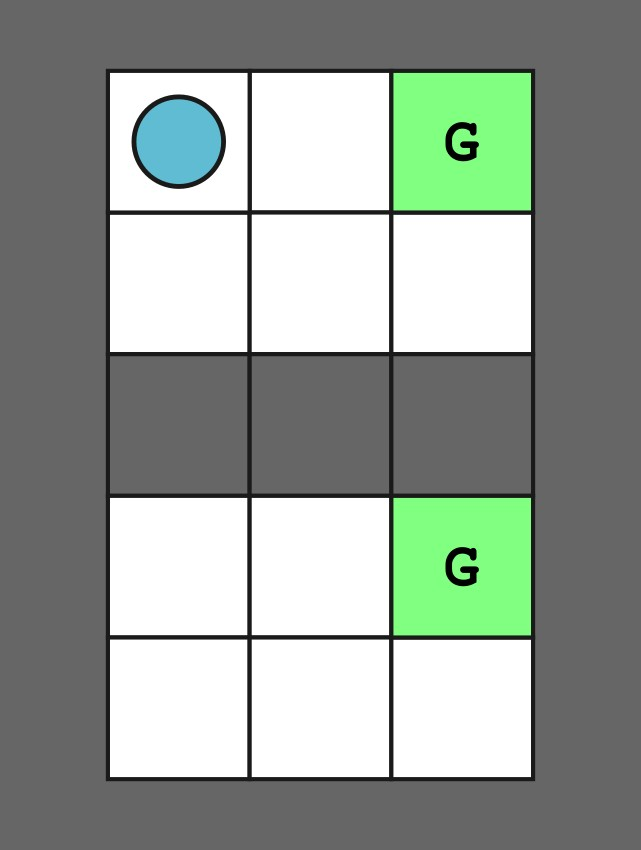
\includegraphics[width=\linewidth]{Figures/grid world.jpg}
        \caption{Grid World}
        \label{fig:grid_world}
    \end{subfigure}
    \hfill
    \begin{subfigure}{0.6\textwidth}
        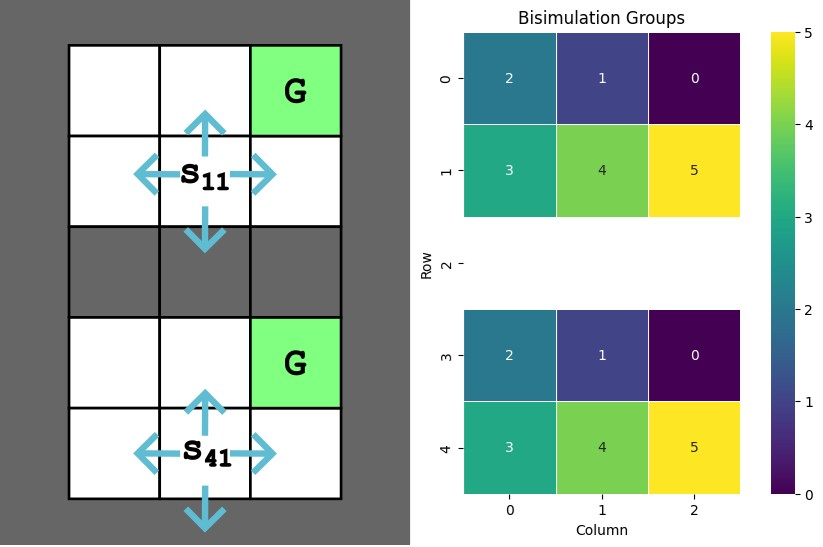
\includegraphics[width=\linewidth]{Figures/bisimulation.jpg}
        \caption{Bisimulation}
        \label{fig:bisimulation_grid_world}
    \end{subfigure}
    \caption[Bisimulation in Grid World]{\textbf{Bisimulation in Grid World}. A basic Grid World illustrating the process of obtaining the largest bisimulation $\sim$, showing the agent (sky blue circle), goals (green G square), transitions, actions, and reward structures, demonstrating how bisimulation captures behavioral similar states into groups of equivalence classes.}

    \label{fig:outdated_priorities}
\end{figure}


However, in reinforcement learning, we are generally more interested in complex behaviors (e.g., high-dimensional states) rather than just symmetrical behaviors. We will progressively analyze more complex behaviors. For now, we start by opening a small passage between the two rooms. When a passage is introduced, the equivalence classes collapse to the identity relation, a trivial solution that is not useful in practice (see Figure \ref{fig:bisimulation_collapse}). This occurs because, as mentioned earlier, bisimulation is a very strong theoretical assumption that requires exact matching of rewards and transitions, which is often challenging to achieve in practice.


% In consequence, the on-policy bisimulation (Definition \ref{def:on-policy-bisimulation}) can be used to only focus on the transition and reward given by the policy action. Notice in the deterministic case, our Grid World, the Equation \ref{eq:on_policy_reward_transition} is reduced too
% \begin{equation}
% \begin{aligned}
% \textbf{Given } a & = \pi(x), \\
% r_x^\pi & = r_x^a \\
% \forall C \in \mathcal{S}_{B^\pi}, \mathcal{P}_x^\pi(C) & = \sum_{x^{\prime} \in C} P_x^a( x^{\prime})
% \end{aligned}
% \end{equation}
% In consequence, it easily to verified that the properties are satisfied, we only have to check one reward and one transition per state in order to hold the reward and transition equivalence properties, and obtain the largest on-policy bisimulation relation $\sim^\pi$. The results are show in the Figure \ref{fig:on_policy_bisimulation}, where we can notice that the on-policy bisimulation effectively reduces the initial MDP of 13 states to and MDP of 4 states. Recall that this method requires to have knowledge of the policy at hand; to showcase the nature of the on-policy bisimulation in its optimal case, we used the optimal policy $\pi^*$ obtained with a value iteration algorithm \cite{sutton2018reinforcement}, but in practice an online policy could be taken into account.

Consequently, the on-policy bisimulation (Definition \ref{def:on-policy-bisimulation}) can be used to focus only on the transitions and rewards determined by a given policy. Notice that, in the deterministic case of our Grid World, Equation \ref{eq:on_policy_reward_transition} simplifies to:

\begin{equation}
\begin{aligned}
\textbf{Given } a &= \pi(x), \\
r_x^\pi &= r_x^a, \\
\forall C \in \mathcal{S}_{B^\pi}, \quad \mathcal{P}_x^\pi(C) &= \sum_{x^{\prime} \in C} P_x^a(x^{\prime}).
\end{aligned}
\end{equation}

Thus, it is easy to verify that the properties are satisfied; we only need to check one reward and one transition per state to ensure the reward and transition equivalence properties hold, allowing us to obtain the largest on-policy bisimulation relation, denoted as $\sim^\pi$. Figure \ref{fig:on_policy_bisimulation} illustrated how the on-policy bisimulation effectively reduces the initial MDP of 13 states to an MDP of 4 states. Note that this method requires knowledge of the policy being used; to demonstrate the on-policy bisimulation in its optimal case, we employed the optimal policy $\pi^*$ obtained using a value iteration algorithm \cite{sutton2018reinforcement}. However, in practice, an online policy could also be considered.

\begin{figure}[h]
    \centering
    \begin{subfigure}{0.45\textwidth}
    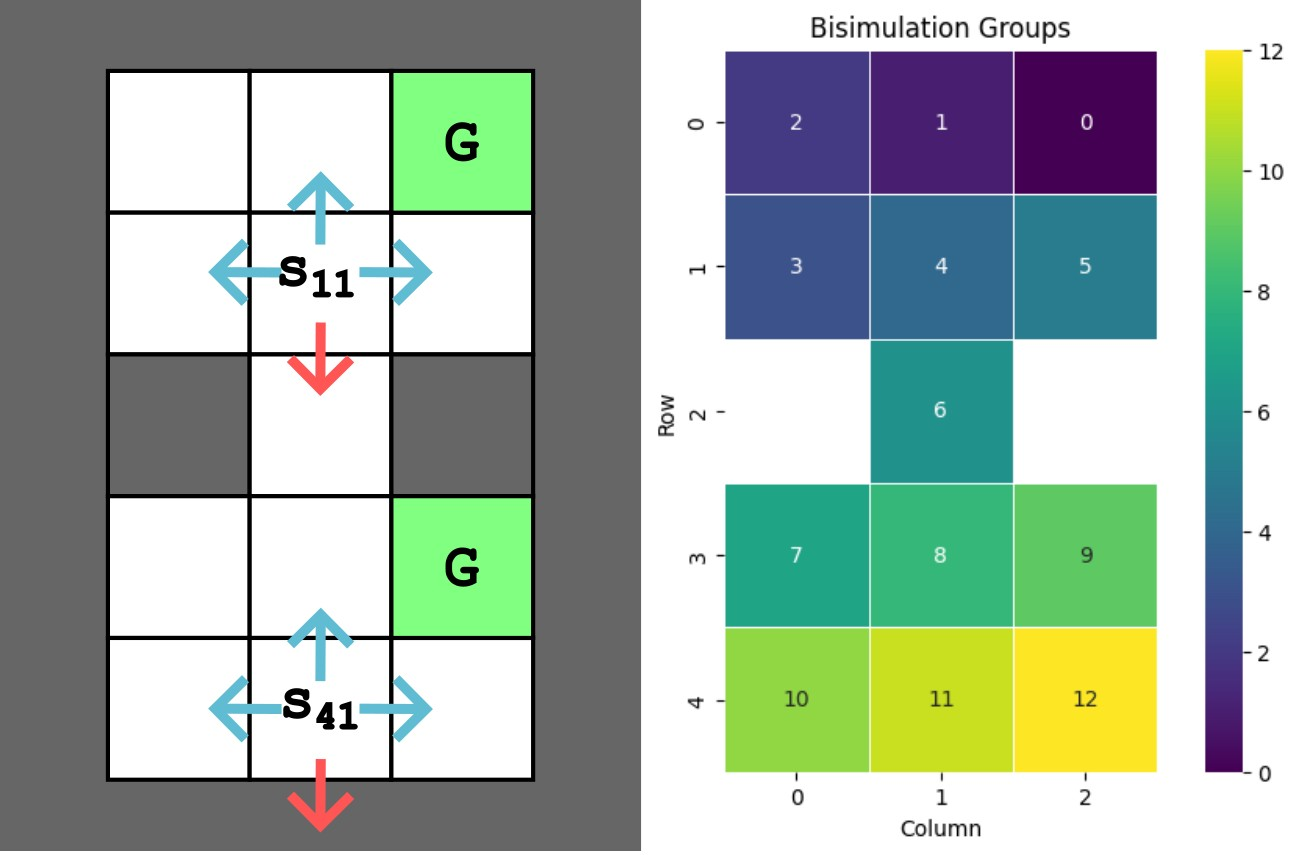
\includegraphics[width=\linewidth]{Figures/bisimulation_passage.jpg}
        \caption{Bisimulation Collapse}
        \label{fig:bisimulation_collapse}
    \end{subfigure}
    \hfill
    \begin{subfigure}{0.45\textwidth}
        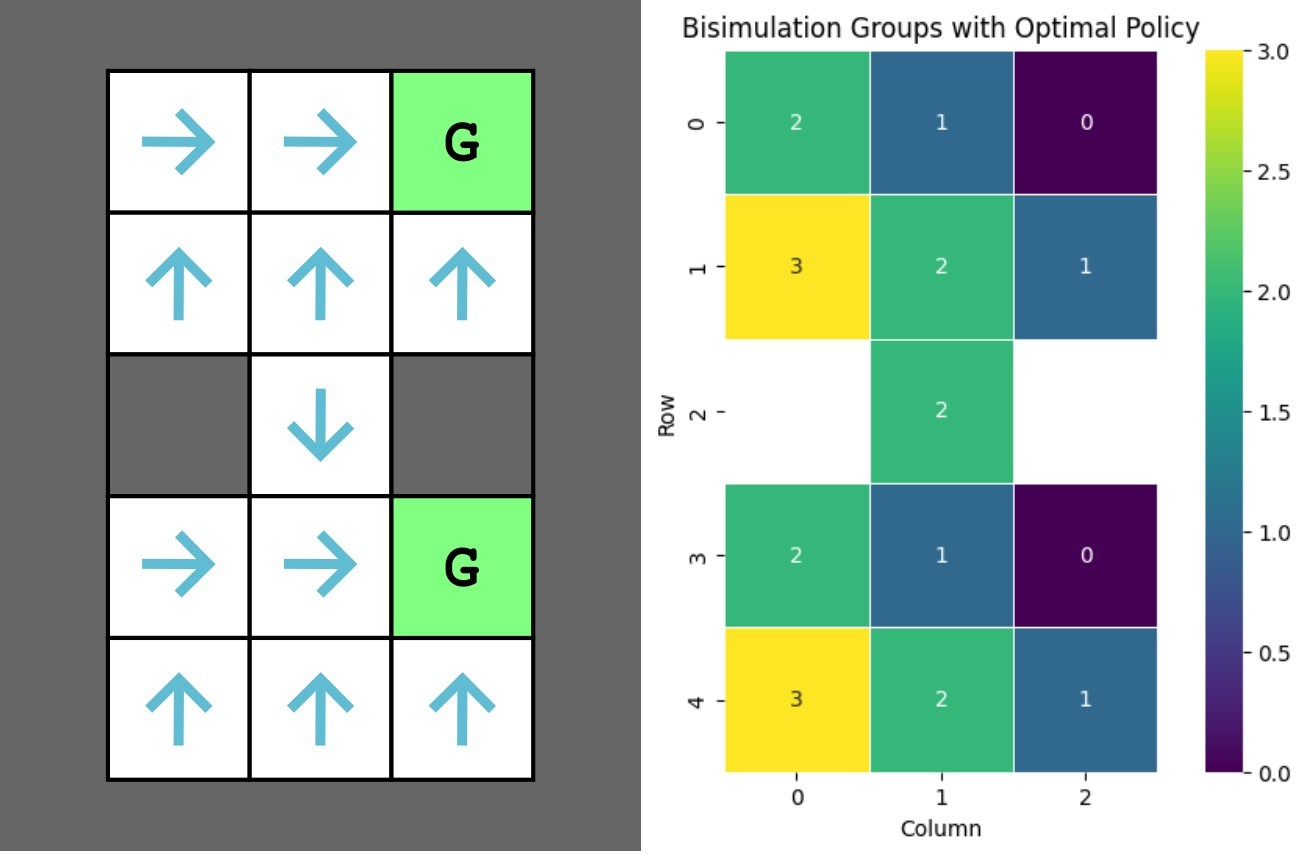
\includegraphics[width=\linewidth]{Figures/on_policy_bisimulation.jpg}
        \caption{On-policy Bisimulation}
        \label{fig:on_policy_bisimulation}
    \end{subfigure}
    \caption[Bisimulation Collapse and On-Policy Bisimulation]{\textbf{Bisimulation Collapse and On-Policy Bisimulation.} (a) Bisimulation collapse caused by the opening of a passage, violating the transitions equivalence between pairs of states, e.g. $s_{11}$, $s_{41}$. (b) A solution provided by on-policy bisimulation, satisfying reward and transition equivalence only for the given policy (denoted by sky blue arrows).}
\end{figure}

% While these groups clearly capture the behavioral similarity of states in the Markov Chain induce by the given policy, they still are not useful in practice for RL, where we are normally estimating things from data, and the calculation of equivalence relation are quite sensitive to infinitesimal variations. In such , we are more interested in provide a notion of behavioral distance from every state vs all the others. The on-policy bisimulation metric in Definition \ref{} provides us the means to do that. Specifically, in our Grid Word, according to Castro \cite{castro2020scalable}, it is possible to reduce the on-policy bisimulation operator to the following operator because our environment is deterministic

While these groups clearly capture the behavioral similarity of states in the Markov chain induced by the given policy, they are still not practical for reinforcement learning, where we commonly estimate values from data, and the calculation of equivalence relations can be highly sensitive to infinitesimal variations. Instead, we are more interested in providing a smoother equivalence notion with the use of behavioral distances from every state to all others. The on-policy bisimulation metric in Definition \ref{def:on_policy_bisimulation_metric} provide us the means to achieve this. Specifically, the deterministic nature of the Grid World allow us to reduce the on-policy bisimulation operator to the operator bellow according to Castro \cite{castro2020scalable}.

\begin{equation}
    \label{eq:deterministic_on_policy_bisimulation_metric}
    T^\pi_k(d)(x, y) = |r^\pi_x - r^\pi_{y}| + \gamma d(x',y') 
\end{equation}

where $x' = \mathcal{N}(x,\pi(x))$ corresponds to the next state given the state $x$ and the action taken by the current policy $\pi(x)$; in other words, $\mathcal{N}$ is a function that deterministically selects the next state with $P(\mathcal{N}(s,\pi(S)) = 1$.

Given that the on-policy operator $T^\pi_k(d)$ is a contraction mapping that converges to a fixed point \(d^\pi_\sim\), we can leverage the recurrence relation over \(d\) in Equation \ref{eq:deterministic_on_policy_bisimulation_metric} to obtain the \textbf{exact on-policy bisimulation metric} through an iterative application of the operator, starting from an initial estimate \(d_0\).

$$d_0 \rightarrow T^\pi_1(d_0) = d_1 \rightarrow T^\pi_2(d_1) = d_2 \cdots \rightarrow d^\pi_\sim$$

Specifically, we can initialize \(d_0\) in a tabular form as a matrix of full zeros, where each cell corresponds to a pair of states in the environment (see Figure \ref{fig:iterative_process}). The updates are then made using a dynamic programming approach by repeatedly applying the following rule:
\begin{equation}
    d_n(x,y) \leftarrow |r_x^a - r_y^a| + \gamma d_{n-1}(x',y'),
\end{equation}
where \(x'\) and \(y'\) are the next states from taking action \(a\) in states \(x\) and \(y\), respectively.

\begin{figure}[h]
    \centering
    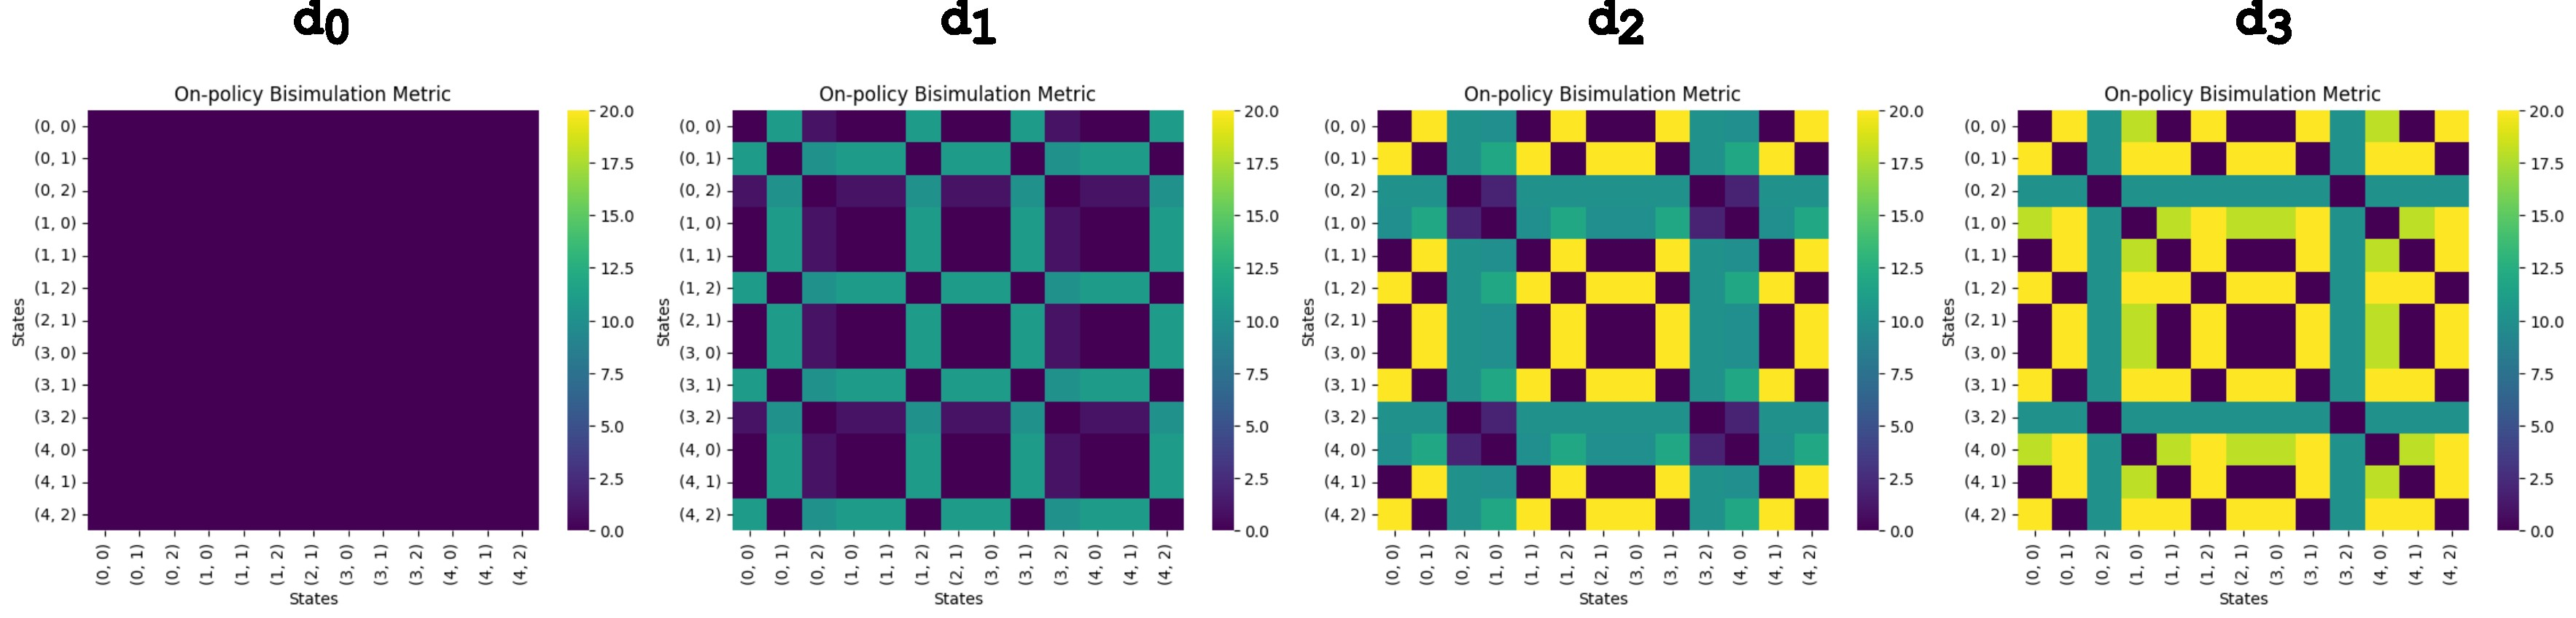
\includegraphics[width=1.\linewidth]{Figures/iterative process.jpg}
    \caption[Recursive On-policy Bisimulation Operator]{\textbf{Recursive On-Policy Bisimulation Operator.} Exact on-policy bisimulation metric through recursive updates of an initial estimate \(d_0\) that converges to \(d_3 = d_\sim^\pi\).}
    \label{fig:iterative_process}
\end{figure}

By applying a Multidimensional Scaling algorithm to the final fixed point distances \(d^\pi_\sim\), we can obtain an approximation of the states in a 2D plane (see Figure \ref{fig:clustering}), effectively clustering states with similar behaviors under a soft notion of distance. It is evident that the on-policy bisimulation distance tends to place behaviorally similar states close together and behaviorally dissimilar states further apart.

\begin{figure}[h]
    \centering
    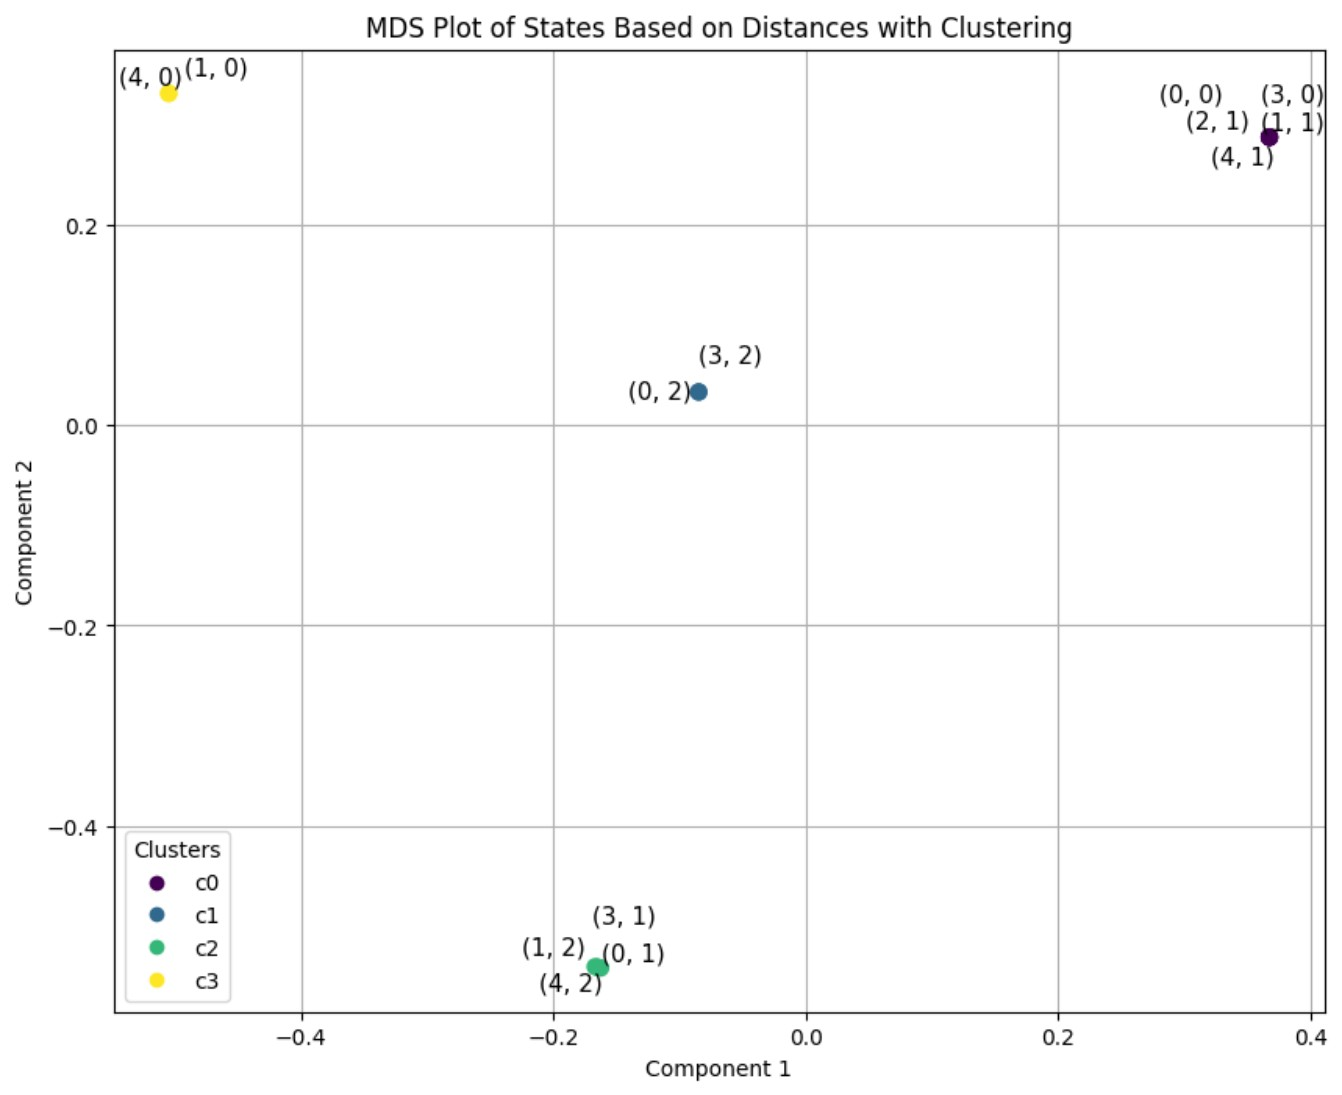
\includegraphics[width=0.9\linewidth]{Figures/clustering.jpg}
    \caption[Multidimensional Scaling of On-policy Bisimulation Distances]{\textbf{Multidimensional Scaling of On-Policy Bisimulation Distances.} The MDS algorithm is applied to on-policy bisimulation distances, revealing clusters of states separated according to the computed distances.}
    \label{fig:clustering}
\end{figure}


% The \textbf{Reward Equivalence}, corresponding to the Equation \ref{eq:reward_equivalence}, corresponds to analyze all the possible transitions between state $s_i$ and $s_j$

In the current work, we are interested in exploring these behaviors in terms of the experiences stored in the experience replay. Note that an experience tuple is defined as \(e_t = (s_t, a_t, r_t, s_{t+1})\). It is evident that experiences with a higher on-policy bisimulation distance between \(s_t\) and \(s_{t+1}\) are likely to be more informative (or 'surprising') than transitions between behaviorally similar states (see Figure \ref{}). By prioritizing transitions with greater behavioral differences, we encourage more diversity in the sampling process. This is the main idea behind our approach. Our method leverages these behavioral distance notions to promote more diverse sampling in the experience replay.

%\subsection{On-policy MICO metric justification}
\section{Bisimulation Prioritized Experience Replay}

The previous example provides a method to calculate the on-policy bisimulation metric in deterministic MDPs and environments with a few states. However, in practice, we often encounter more complex environments with high-dimensional representations (e.g., pixels), where calculating on-policy bisimulation metrics in a tabular form becomes intractable.

To address these challenges, we employ an indirect approach to approximate these bisimulation metrics within the RL loop. Specifically, works by Zhang et al. \cite{zhang2020learning} and Castro et al. \cite{castro2021mico} have demonstrated that it is more effective and general to obtain a bisimulation metric as part of the online learning of state abstractions. In the following, we will detail the specific method for learning these abstractions and how this approach allows us to approximate the metric on the fly.

\subsection{Learning State Abstractions}

The present work employs a surrogate on-policy bisimulation metric known as the MICO metric \cite{castro2021mico} (see Definition \ref{def:mico_operator}). The MICo metric substitutes the Kantorovich distance $\mathcal{W}_d$ calculation with the independent coupling. For reference, we restate the operator equation here:
$$
\label{eq:mico_operator}
    T^\pi_M(U)(x, y) = |r^\pi_{x} - r^\pi_{y}| + \gamma \mathbb{E}_{x'\sim P_x^\pi, y'\sim P_y^\pi}\left[U(x',y') \right]
$$

% , where the first term corresponds to the reward equivalence difference, and the second corresponds to the independent coupling.

The MICo operator is used to learn a parameterized state abstraction \(\phi_\omega(x) : \mathcal{S} \to \mathcal{S}_\phi\) (parameterized by \(\omega\)), which maps a true environmental state (e.g., pixels) to a lower-dimensional latent representation. The goal is to position these representations in such a way that a chosen parameterized distance $U_\omega(x,y)$ (e.g., Euclidean, cosine) coincides with the MICo distance in the latent space (see Figure \ref{}). However, since the MICo distance is a diffuse metric (see Definition \ref{def:diffuse_metric}), the parameterized distance must ensure positive self-distances. To achieve this, the following parameterized distance function was proposed in \cite{castro2021mico} for any \(x, y \in \mathcal{S}\):
\begin{equation}
    U^\pi(x, y) \approx U_\omega(x, y):=\frac{\left\|\phi_\omega(x)\right\|_2^2+\left\|\phi_\omega(y)\right\|_2^2}{2}+\beta \theta\left(\phi_\omega(x), \phi_\omega(y)\right)
\end{equation}

where the first term ensures positive self-distances\footnote{In theory, the second term can be any other notion of distance, such as the euclidean distance. However, empirical results from MICo\cite{castro2021mico} have shown that the angular distance provides greater numerical stability.}, $\phi_\omega(x), \phi_\omega(y)$ corresponds to the abstract representations, $\theta\left(\phi_\omega(x), \phi_\omega(y)\right)$ is the angle between vectors $\phi_\omega(x)$ and $\phi_\omega(y)$, and $\beta$ is an hyperparameter.

Consequently, the recursive nature of the operator \(T_M^\pi(U)(x,y)\) is used to define a loss function, which works similarly to the Bellman recurrence process in DQN. In this approach, a target is defined, and we aim to approximate this target with a online estimate. Specifically, in our case, the loss function measures the difference between a learning target MICo metric\footnote{\(U_{\bar{\omega}}\) is an unbiased estimator of the independent coupling.} \(T_{\bar{\omega}}^U\) and the online MICo metric \(U_\omega\), as 

\begin{equation}
\label{eq:mico_loss}
    \mathcal{L}_{\mathrm{MICo}}(\omega)=\mathbb{E}_{\left\langle x, r_x, x^{\prime}\right\rangle,\left\langle y, r_y, y^{\prime}\right\rangle}\left[\left(T_{\bar{\omega}}^U\left(r_x, x^{\prime}, r_y, y^{\prime}\right)-U_\omega(x, y)\right)^2\right]
\end{equation}

\begin{equation}
    T_{\bar{\omega}}^U\left(r_x, x^{\prime}, r_y, y^{\prime}\right)=\left|r_x-r_y\right|+\gamma U_{\bar{\omega}}\left(x^{\prime}, y^{\prime}\right)
\end{equation}

where \(\bar{\omega}\) is a separate copy of the network parameters, synchronized with \(\omega\) at infrequent intervals, and the pairs of transitions \(\left\langle x, r_x, x^{\prime}\right\rangle\) and \(\left\langle y, r_y, y^{\prime}\right\rangle\) are sampled from the experience replay.\footnote{The actions are not considered in the experiences because we assume a fixed policy under the on-policy assumption.} \footnote{When distances are large, they can oversaturate the MICo loss, causing instability in gradient updates. Therefore, in practice, a Huber loss is employed to focus on small differences between states.}

The MICO learning can be integrated into any value-based agent by learning an estimate $Q_{\xi, \omega}(x, \cdot) = \psi_\xi(\phi_\omega(x))$, where $\phi_\omega(x)$ corresponds to the representation of state $x$, and $\psi_\xi$ corresponds to the value approximator. This work specifically focuses on the DQN algorithm (see Section \ref{sec:dqn}), where the $Q_{\xi, \omega}$ corresponds to the Q-values. In this scenario, the MICO loss $\mathcal{L}_{\text{TD}}$ is combined with the temporal-difference loss $\mathcal{L}_{\text{MICo}}$ as 
\begin{equation}
    \mathcal{L}_\alpha(\xi, \omega) = (1 - \alpha)\mathcal{L}_{\text{TD}}(\xi, \omega) + \alpha \mathcal{L}_{\text{MICo}}(\omega)
\end{equation}
, where $\alpha \in (0, 1)$. 
Figure \ref{} illustrates the network architecture used for learning, showing that the MICo loss is applied directly after the convolution layers and used to calculate the total loss $\mathcal{L}_\alpha$. Note that the same parameters $\omega$ are shared for both losses and both inputs, without the need for additional parameters.


% Additionally, notice the network are identical for both only the inputs are different. In such way, no extract parameters are used to learn the representation

Although the MICo loss $\mathcal{L}_{\text{MICo}}$ requires pairs of transitions $\left\langle x, r_x, x^{\prime}\right\rangle$ and $\left\langle y, r_y, y^{\prime}\right\rangle$, in practice, transitions are not sampled as pairs; we only have access to a mini-batch of unpaired transitions, necessitating a method to pair them. To address this issue, a \textbf{squarify} method \cite{castro2020scalable} was proposed to construct pairs of transitions by pairing each transition with all others within the current mini-batch and then calculating the MICo loss. Figure \ref{} illustrates how this squarify process works.

% Then, the metric is used as part of a loss function to learn state abstractions.  Specifically, in this work, an encoder will map high-dimensional states (e.g., frames from an RL environment) into a lower-dimensional latent space, such that behaviorally similar states are kept closer together and behaviorally dissimilar states are kept farther apart in the latent space.

\subsection{Priority Strategies}


In the following, we propose our method, \textbf{Bisimulation Prioritized Experience Replay (BPER)}, along with \textbf{two strategies} for calculating these priorities on the fly, based on certain hypotheses. As mentioned before, the MICo metric is approximated online as part of the state abstraction learning process, so that it is enough to use $U_\omega$ to calculate a MICo distance between two states and update the priorities accordingly.

Another possible option for calculating the distance online is to use the target distance \(T^U_{\bar{\omega}}\), which uses the corresponding rewards difference. However, since the metric will eventually converge to a fixed point, it is sufficient and more convenient to use \(U_\omega\), as this approach does not require incorporating rewards into its calculation.

% \subsubsection{Strategy 1: Current vs Next (BPERcn)}

\begin{strategy}[\textbf{Current vs Next: BPERcn}]
Consider a current minibatch \(B \subset \mathcal{E}\), $|B| = k$, containing transition experiences \(e_i = (s_i, r_i, a_i, s_{i+1})\). Each transition can be associated with a distance \(U_\omega(s_i, s_{i+1})\), which effectively quantifies how behaviorally different the \textbf{current state} \(s_i\) is compared to the \textbf{next state} \(s_{i+1}\). Consequently, the re-weighted priority is calculated as follows:

\begin{equation}
    p_i = (1 - \mu) |\delta_i| + \mu U_\omega(s_i, s_{i+1}) + \epsilon,
\end{equation}

where \(\delta_i\) corresponds to the TD-error of the experience, \(\mu \in [0,1)\) controls the balance between the TD-error and the bisimulation distance, and \(\epsilon\) is a small positive constant to ensure that experiences are revisited even when the weighted priority is equal zero.
\end{strategy}

The distance \(U_\omega(s_i, s_{i+1})\) serves as an indicator of a 'surprising' transition, suggesting that transitions with larger distances are more informative and likely to contribute to greater learning progress. While using TD-error as an standalone method could potentially overemphasize some transitions, leading to a loss of diversity \cite{schaul2015prioritized},\cite{pan2022understanding},\cite{fedus2020revisiting}, our method consistently encourages diversity in the experiences by reweighting the TD-error, regulated by a parameter $\eta \in [0,1)$.

Similar to a proportional prioritization in PER \cite{schaul2015prioritized} (see Section \ref{sec:per}), the sampling probability for an experience $e_i$ is given by $P(t) = \frac{p_t^\alpha}{\sum_k p_k^\alpha}$, where $\alpha$ controls the degree of prioritization. Additionally, the weighted importance sampling for unbiased updates is computed as $w_i = \left(\frac{1}{N} \cdot \frac{1}{P(i)} \right)^\beta$, followed by a normalization step $\frac{1}{\max_k w_k}$. In practice, a sum tree data structure is used to optimize the sampling procedure.
% \subsubsection{Strategy 2: All vs All (BPERaa)}

Strategy 1 provides a theoretical valid method to characterize the priority of transition based on a behavioral distance between the current and next state. However, in practice, the trajectories may overlap significantly, resulting in \textbf{overlapping states distributions} with highly similar behaviors. Additionally, since the bisimulation is approximated online, there are sources of variability in the approximation until reaching the convergence point. These issues can trigger trajectories with many similar distances between current and next states (see Figure \ref{}), with only a few behavioral different states appearing after long rollouts; resulting in scarce high-priority transitions, and consequently affecting the effectiveness of prioritization technique. To address these issues, the following empirical solution is proposed. 

\begin{strategy}[\textbf{All vs All: BPERaa}]
Consider a minibatch $B \subset \mathcal{E}$, $|B| = k$, with transition experiences $e_i = (s_i, r_i, a_i, s_{i+1})$. Each transition $e_i$ can be associated with a relative bisimulation distance

\begin{equation}
    U^B_\omega(s_i) = \sum_{i=1}^k U_\omega(s_i, s_k), \quad \forall e_k = (s_k, r_k, a_k, s_{k+1}) \in B
\end{equation}

Consequently, the re-weighted priority will be calculated as follows

\begin{equation}
    p_i = (1 - \mu) |\delta_i| + \mu U^B_\omega(s_i) + \epsilon
\end{equation}
where \(\delta_i\) corresponds to the TD-error of the experience, \(\mu \in [0,1)\) controls the balance between the TD-error and the bisimulation distance, and \(\epsilon\) is a small positive constant to ensure that experiences are revisited even when the weighted priority is equal zero.
\end{strategy}


Although the current states from different transitions are not directly connected by a valid transition, the bisimulation metric allows us to measure behavioral dissimilarity between all states in the environment. This enables the calculation of a behavioral distance relative to the current minibatch by computing the mean distance between each current state and all other states in the minibatch (see Figure \ref{}). This relative distance serves as a smoother indicator of how behaviorally dissimilar one initial state is compared to the others, indicating 'surprising' or more informative transitions. Figure \ref{} illustrates how the initial states of all transitions in the minibatch are positioned in the latent space, with more behaviorally distinct states placed farther apart. In practice, we use the squarify method, along with reshaping and averaging operations, to compute these distances on the fly. Similar as before, the $\alpha$-priority, weighted importance sampling and sum tree data structure are used for the sampling procedure.

Algorithm \ref{algorithm:dqn_bper} illustrates the entire prioritizing process, highlighting the modifications made to the original and prioritized version. Similar to the PER method the priorities are only updated for the current sampled mini batch to maintain computational efficiency. Notice the algorithm depicts the procedure for Strategy 1 (BPERcn). Strategy 2 (BPERaa) requires a minor replacement in line 19, where \(U_\omega(s_i, s_{i+1})\) should be replaced with \(U^B_\omega(s_i)\). An additional algorithm illustrating only MICo learning with DQN, without BPER, is provided in Appendix \ref{} for reference.

\begin{algorithm}
\caption{DQN with Bisimulation Prioritized Experience Replay (BPERcn)}
\label{algorithm:dqn_bper}
\begin{algorithmic}[1]
\State \textbf{Input:} minibatch $k$, step-size $\eta$, replay period $K$ and size $N$, exponents $\alpha$ and $\beta$, budget $T$ (total steps), priority weigh $\mu$.
\State \textbf{Initialize} action-value function $Q$ with random weights $\xi$, $\omega$
\State \textbf{Initialize} target action-value function $Q^-$ with weights $\{\bar{\xi},\bar{\omega}\} \leftarrow \{\xi, \omega\}$
\State \textbf{Initialize} replay memory $\mathcal{D} = \emptyset$ with capacity $N$, $p_1 = 1$ (inital priority) %$\Delta_{\{\xi, \omega\}} = 0$, $\Delta_\omega = 0$, $p_1 = 1$
% \State Observe $s_0$ and choose $a_0 \sim \pi^\epsilon_\theta(s_0)$ 
\For{$t = 1$ to $T$}
    \State Observe $s_t$
    \State Choose action $a_t \sim \pi^\epsilon_\theta(s_t)$
    \State Execute action $a_t$ and observe $r_t$ and $s_{t+1}$
    \State Store transition $(s_t, a_t, r_t, s_{t+1})$ in $\mathcal{D}$ with maximal priority $p_t = \max_{i < t} p_i$
    \If{$t \equiv 0 \mod K$}
        % \For{$j = 1$ to $k$}
        \State Sample minibatch $B$ of transitions $e_j$ with probability $P(j) = \frac{p_j^\alpha}{\sum_i p_i^\alpha}$    
        \State Compute importance-sampling weight $w_j = \left( N \cdot P(j) \right)^{-\beta} / \max_i w_i$
        \State Set $y_j = 
        \begin{cases} 
            r_j & \text{for terminal } s_{j+1}\\
            r_j + \gamma \max_{a'} Q^-(s_{j+1}, a'; \{\bar{\xi},\bar{\omega}\}) & \text{otherwise}
        \end{cases}$
        \State Compute TD-error $\delta_j = y_j - Q(s_{j}, a_{j}; \{\xi, \omega\})$, and loss $\mathcal{L}_{\text{TD}} = \delta_j^2 $
        \State Squarify minibatch $B$ to get transition pairs $\left\langle x, r_x, x^{\prime}\right\rangle,\left\langle y, r_y, y^{\prime}\right\rangle$ 
        \State Compute MICo loss $\mathcal{L}_{\text{MICo}} = \left(T_{\bar{\omega}}^U\left(r_x, x^{\prime}, r_y, y^{\prime}\right)-U_\omega(x, y)\right)^2$
        \State Compute total loss $\mathcal{L}_\alpha(\xi, \omega) = (1 - \alpha) \mathcal{L}_{\text{TD}}(\xi, \omega) + \alpha \mathcal{L}_{\text{MICo}}(\omega)$
        \State Perform a gradient descent step on $\mathcal{L}_\alpha(\xi, \omega)$, weighting the updates by $w_j$
        \State Update transition priority $p_j \leftarrow (1 - \mu) |\delta_j| + \mu U_\omega(s_j,s_{j+1}) + \epsilon$
        \State Every C optimizing steps update $\{\bar{\xi},\bar{\omega}\} \leftarrow \{\xi, \omega\}$
        

        
        % \State Accumulate weight-change $\Delta_{\{\xi, \omega\}} \leftarrow \Delta_{\{\xi, \omega\}} + w_j \cdot \delta_j \cdot \nabla_\theta Q(s_{j}, a_{j})$
        % \State Compute bisimulation distance error $\sigma_j = T_{\bar{\omega}}^U\left(r_x, x^{\prime}, r_y, y^{\prime}\right)-U_\omega(x, y)$
        %  \State Accumulate weight-change $\Delta_{\omega} \leftarrow \Delta_{\omega} + w_j \cdot \sigma_j \cdot \nabla_\omega U_\omega(s_{i}, a_{j})$   

        % \EndFor
        % \State Update weights $\theta \leftarrow \theta + \eta \cdot \Delta$, reset $\Delta = 0$
    \EndIf
\EndFor
\end{algorithmic}
\end{algorithm}

\section{Experimentation Setup}

% \subsection{Experiments and Environments}
The proposed method will be tested in two setups: 1) 31-state Grid Worlds illustrated in Figure \ref{fig:behavioral_similarity}; similar to those environment in the works of Pan et al. \cite{pan2022understanding} and Castro \cite{castro2020scalable}, where calculating the bisimulation metrics is relatively straightforward; and 2) the Classic Control benchmark suite\footnote{Classic Control benchmark: \href{https://www.gymlibrary.dev/environments/classic_control/}{https://www.gymlibrary.dev/environments/classic\_control/}}, and the Lunar Lander from the Box2D suite\footnote{Box2D suit benchmark: \href{https://gymnasium.farama.org/environments/box2d/}{https://gymnasium.farama.org/environments/box2d/}}. In these setups, states will be \textbf{partially observable derived from pixels}, rather than full descriptive states.

The experiments aims to validate our proof of concept rather than test state-of-the-art results. Although the Grid Word is trained using pixels-based states, the underlying 31-state MDP enable us to measure evaluation metrics without high computational cost. Specifically, we will use the Grid World to evaluate our algorithm's performance on three key problems:

\begin{itemize}
    \item First, to evaluate the \textbf{task-agnostic sampling} problem, we examined how well the algorithm prioritizes behaviorally dissimilar states by showing distributions of priorities and behavioral similarities, similar to the experiments in Castro's work \cite{castro2020scalable}.

    \item Second, to evaluate the \textbf{outdated priorities} problem, we replicated the sampling distribution experiments from Pan et al.'s work \cite{pan2022understanding}. The purpose of this experiment is to assess how closely the priorities updated per minibatch align with the ideal case, where the priorities of the entire state space are updated at each time step. To measure this, we used two distance schemes proposed in Pan et al.'s work \cite{pan2022understanding}.

    Given the sampling distribution of priorities \(p_i(\cdot)\) from the experience buffer and the corresponding ideal distribution \(p_i^*(\cdot)\) (theoretically achieved when all state space priorities are updated at each time step\footnote{While the ideal distribution represents the best-case scenario, it is impractical to update all possible state priorities under the current policy at each step in practice.}), 1) the on-policy weighting is given by \(\sum_{j=1}^{31} w^\pi(s_j) | p_i(s_j) -p_i^*(s_j)|, i \in \{1,2\}\), and 2) the uniform weighting is \(\frac{1}{31} \sum_{j=1}^{31} | p_i(s_j) -p_i^*(s_j) |, i \in \{1,2\}\), where \(p_1\) corresponds to the PER method and \(p_2\) corresponds to the BPER method. A more detailed explanation of this procedure is provided in the Appendix \ref{}.
    
    \item Third, to evaluate \textbf{state space coverage}, we visually and quantitatively assessed the level of exploration per algorithm. We plotted the distribution of visited states in our Grid Worlds, similar to \cite{pan2022understanding}, and calculated the corresponding entropy of the state visitation distribution as $H(\mathcal{S}) = - \sum_{i=1}^{|\mathcal{S}|} p(s_i) \log p(s_i)$, where \(p(s_i)\) is the probability of visiting state \(s_i\), calculated as the ratio of visits to state \(s_i\) over the total number of visits to all states.
\end{itemize}


Finally, we performed standard test (time steps vs. episodic reward) to compare our algorithm's performance against standard ER and Prioritized ER in slightly more complex environments, such as: Cartpole, Mountain Car, Acrobot, and LunarLander, using pixel-based states. As many episodic reward results overlap, we decided to plot the \textbf{Episode Reward Gain} by comparing the methods PER, BPERaa, and BPERcn against two baselines: DQN and DQN + MICo. The Episode Reward Gain is calculated per episode as follows: \(\mathcal{R}^G(\tau) = \mathcal{R}_{\text{method}}(\tau) - \mathcal{R}_{\text{baseline}}(\tau)\), where \(\tau\) can correspond to trajectories of different lengths\footnote{To handle these differences, we use back and forward filling for NaN values in the episodic reward trajectory results.}. A positive Episode Reward Gain indicates an improvement over the baseline, while a negative value indicates underperformance compared to the baseline.

The RL algorithm used for all our experiments was DQN \cite{mnih2013playing}, with extensions added in a plug-in fashion while maintaining consistent hyperparameters across different environments and algorithms to ensure fair comparisons. For PER and MICo state-of-the-art hyper-parameters were used, extracted from the original papers, and only a sweep over the newly introduced hyperparameter \(\nu\) was conducted for the 31-state Grid World. A detailed explanation of the hyperparameters used is provided in Appendix \ref{}.

The algorithms were implemented using the TorchRL library\footnote{TorchRL: \href{https://pytorch.org/rl/stable/index.html}{https://pytorch.org/rl/stable/index.html}}. Specifically, the baseline DQN algorithm was taken from the SOTA implementations available at the \href{https://github.com/pytorch/rl/tree/main/sota-implementations/dqn}{TorchRL GitHub repository}, and the corresponding extensions (PER, MICo, MICo + BPER) were developed and added. The MICO extension was reproduced on TorchRL based on the original repository: \href{https://github.com/google-research/google-research/tree/master/mico}{Google Research MICO}. The experiments were executed on an RTX 4060 GPU with 8GB of memory. The algorithm is accessible through the university GitLab and a \href{https://github.com/ZosoV/final_project}{personal GitHub}.
% \subsection{TorchRL}




% % !TEX root =  ../Dissertation.tex

\chapter{Results and Discussion}

In this section, it is presented a series of experiments done in different RL environments. Particularly, a 31-state simple GridWorld was used as proof of concept to analyze the efficient of our method by evaluating three keys problems in non-uniform sampling methods, such as task-agnostic sampling, outdated priorities, and state space coverage. After exploring these main issues, a general evaluation on slightly more complex was done to measure the performance of our algorithm in the RL scenario.

\section{Grid World - Episode Reward}

Episode Reward and Cumulative Reward were initially chosen to indicate the performance during training of different DQN extensions. The full priority weighting (weight: 1.0) version was used for BPERcn and BPERaa alternatives, such that it only prioritizes with bisimulation distances and not td-error. The algorithm was executed for 5 independent executions and the mean, min and max values (bottom and upper margin of shaded regions) per time steps are show in Figure \ref{fig:episode_cumulative_reward}. The methods DQN and DQN + MICO work as baseline to compare all other methods. 


Figure \ref{fig:episode_reward_grid_world} illustrates the episode reward per time steps during training, calculated in a 100 steps average window. While all methods show an improvement over time, converging after 100k steps, both BPERcn and BPERaa show promising improvements early in the training process, obtaining better performance than baselines and PER extension. However, over time, BPERaa keeps more consistent and stable improvements, indicating a better manage of priorities in the experience replay, while BPERcn shows a decrease of performance after the time step 30k. This results suggest that the smoother relative strategy 2, BPERaa, could in fact be beneficial in practice. Additionally, even though the GridWorld is a simple environment, the PER alternative under performs against all the other methods over time, showing the effectiveness of prioritizing behavioral dissimilar states.

The cumulative reward in Figure \ref{fig:cumulative_reward} helps us to check the overall time collected reward, a higher value will indicate a better ability to follow actions that leads to positive rewards. This complementary information indicates us that BPERaa in fact produces a policy that collect higher rewards, increasing the performance over the direct baseline DQN + MICO, which effectively show us that BPERaa is in fact making a positive effect in improving DQN + MICO. Alternatively, the other strategy, BPERcn, shows improvements in the earlier stages of learning, but eventually start decreasing the performance (around the 50k step) making the DQN + MICO reward acquisition worse, but keeping a similar performance that the baseline DQN. Overall, the PER alternative is the worse having difficulties to collect the rewards and in fact hindering the learning of the baseline DQN. 

\begin{figure}[h]
    \centering
    \begin{subfigure}{0.45\textwidth}
    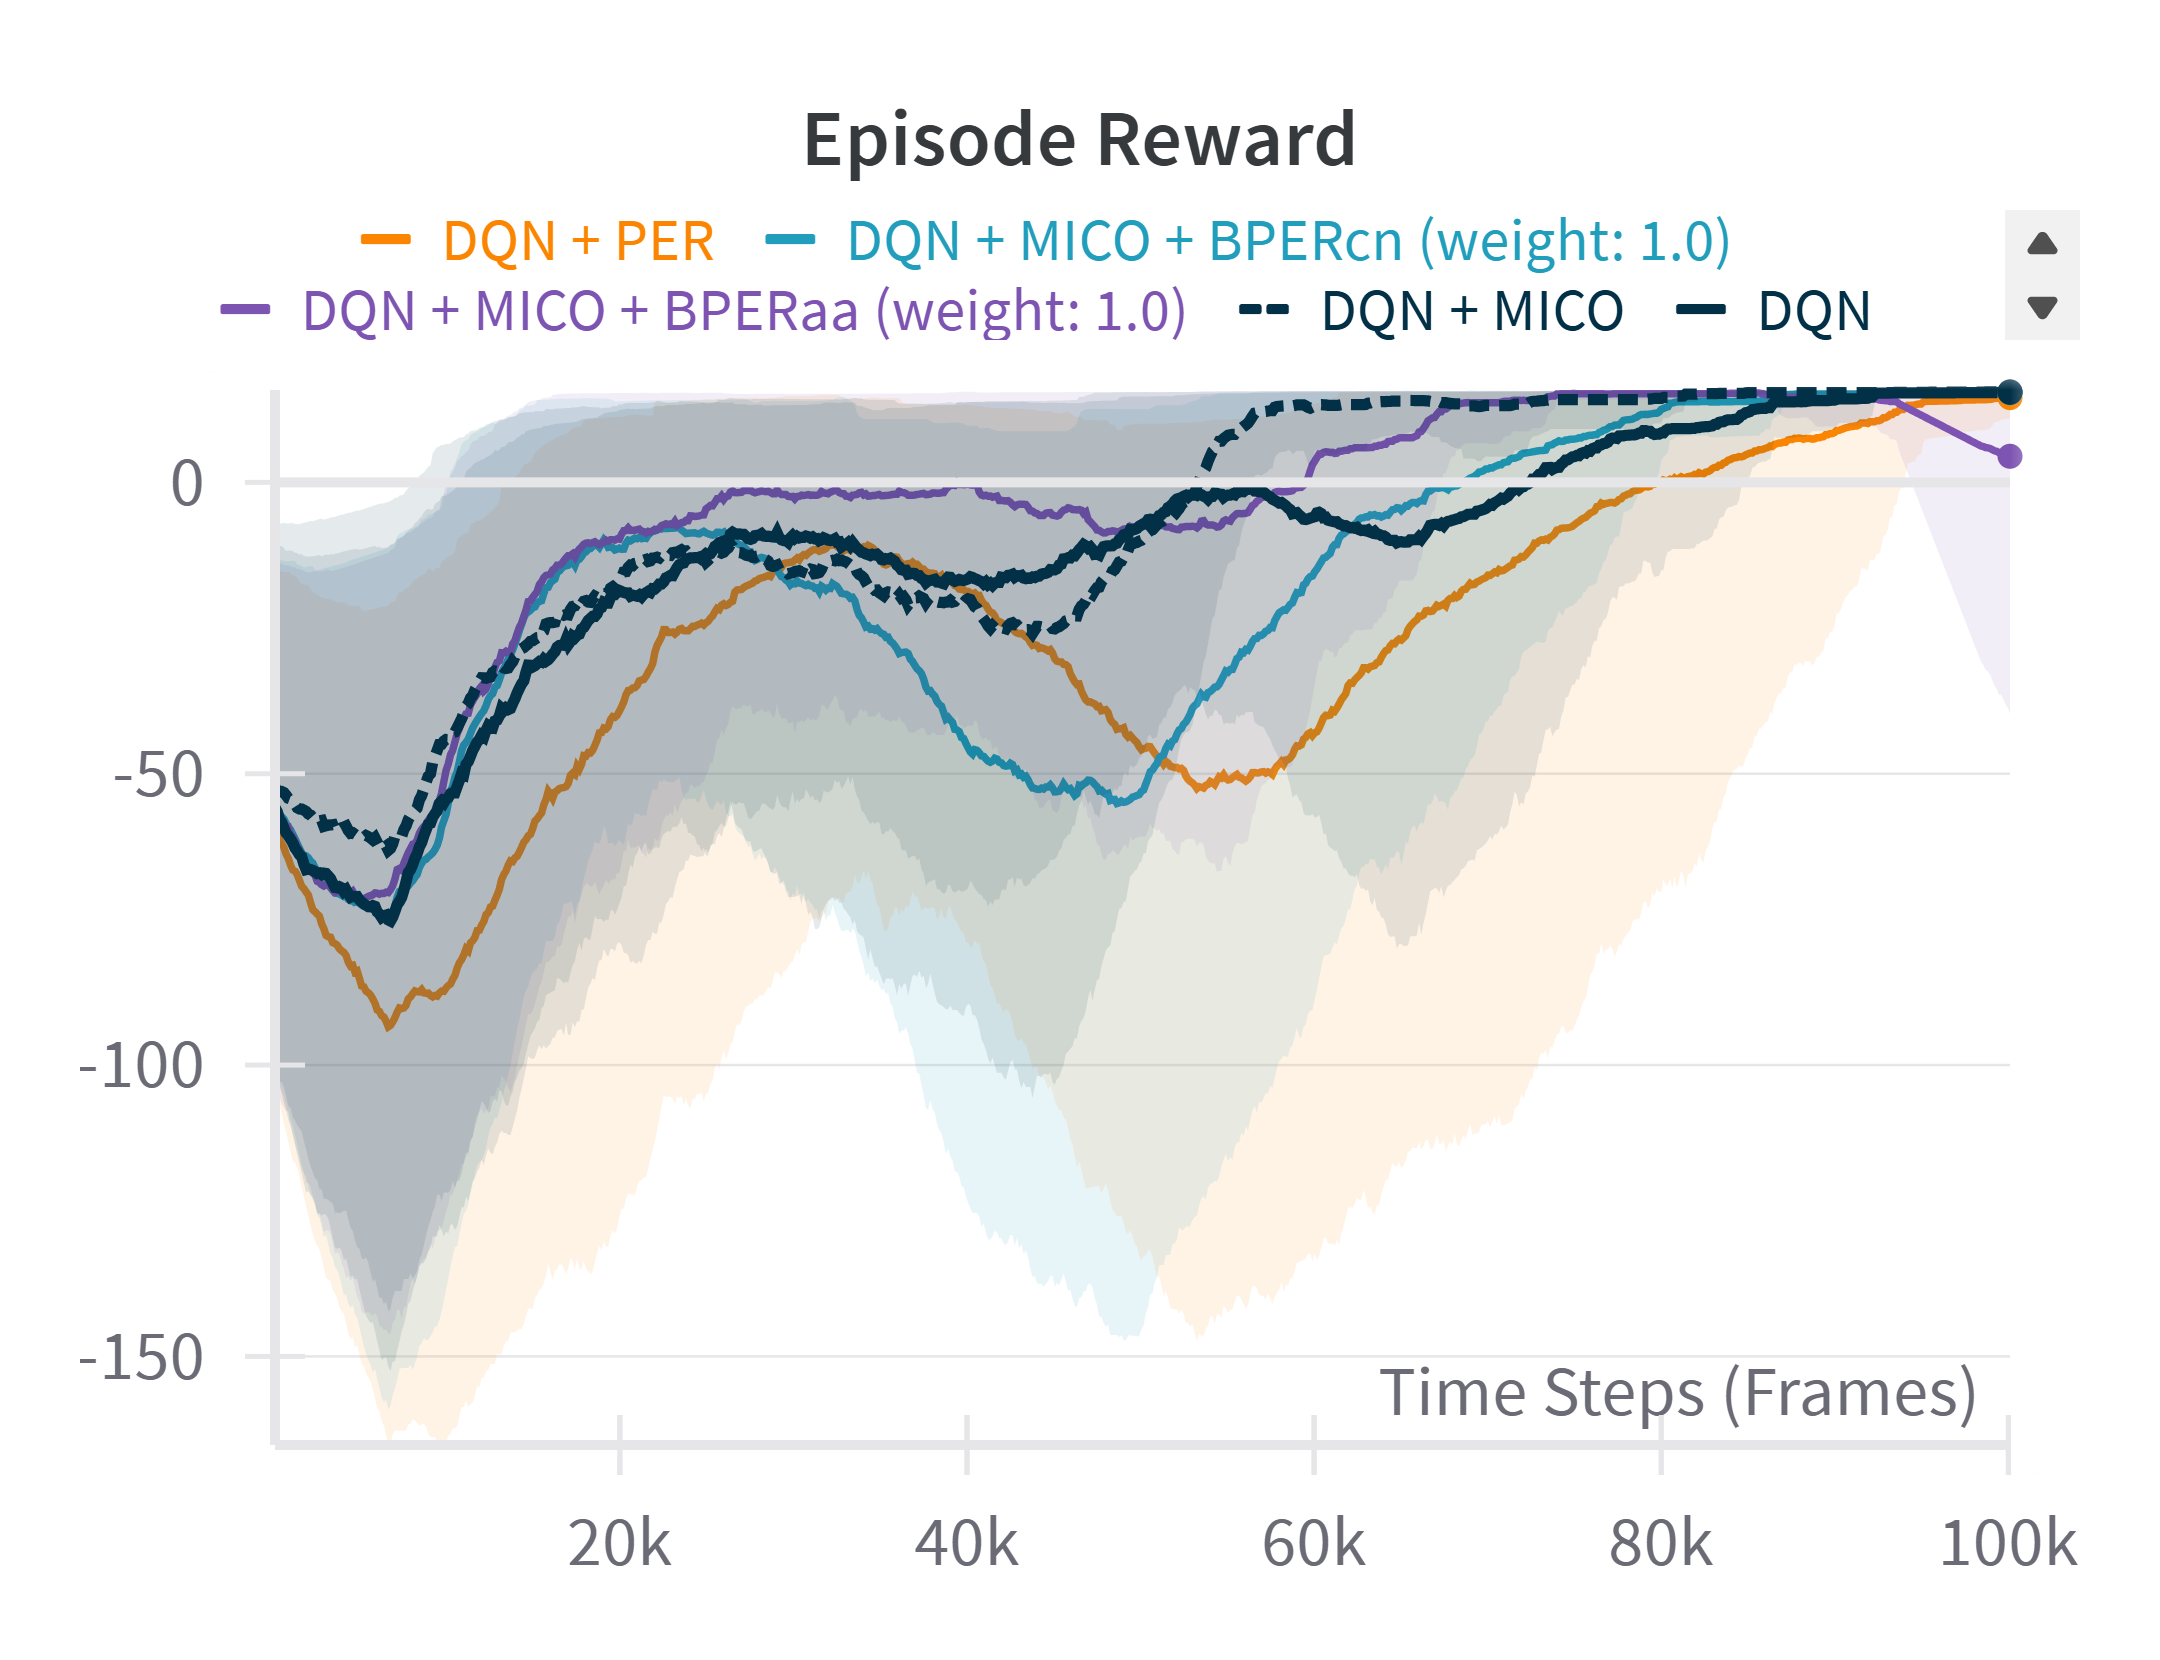
\includegraphics[width=\linewidth]{Results/grid_world/episode_reward_grid_world_window_100.png}
        \caption{Episode Reward}
        \label{fig:episode_reward_grid_world}
    \end{subfigure}
    \hfill
    \begin{subfigure}{0.45\textwidth}
        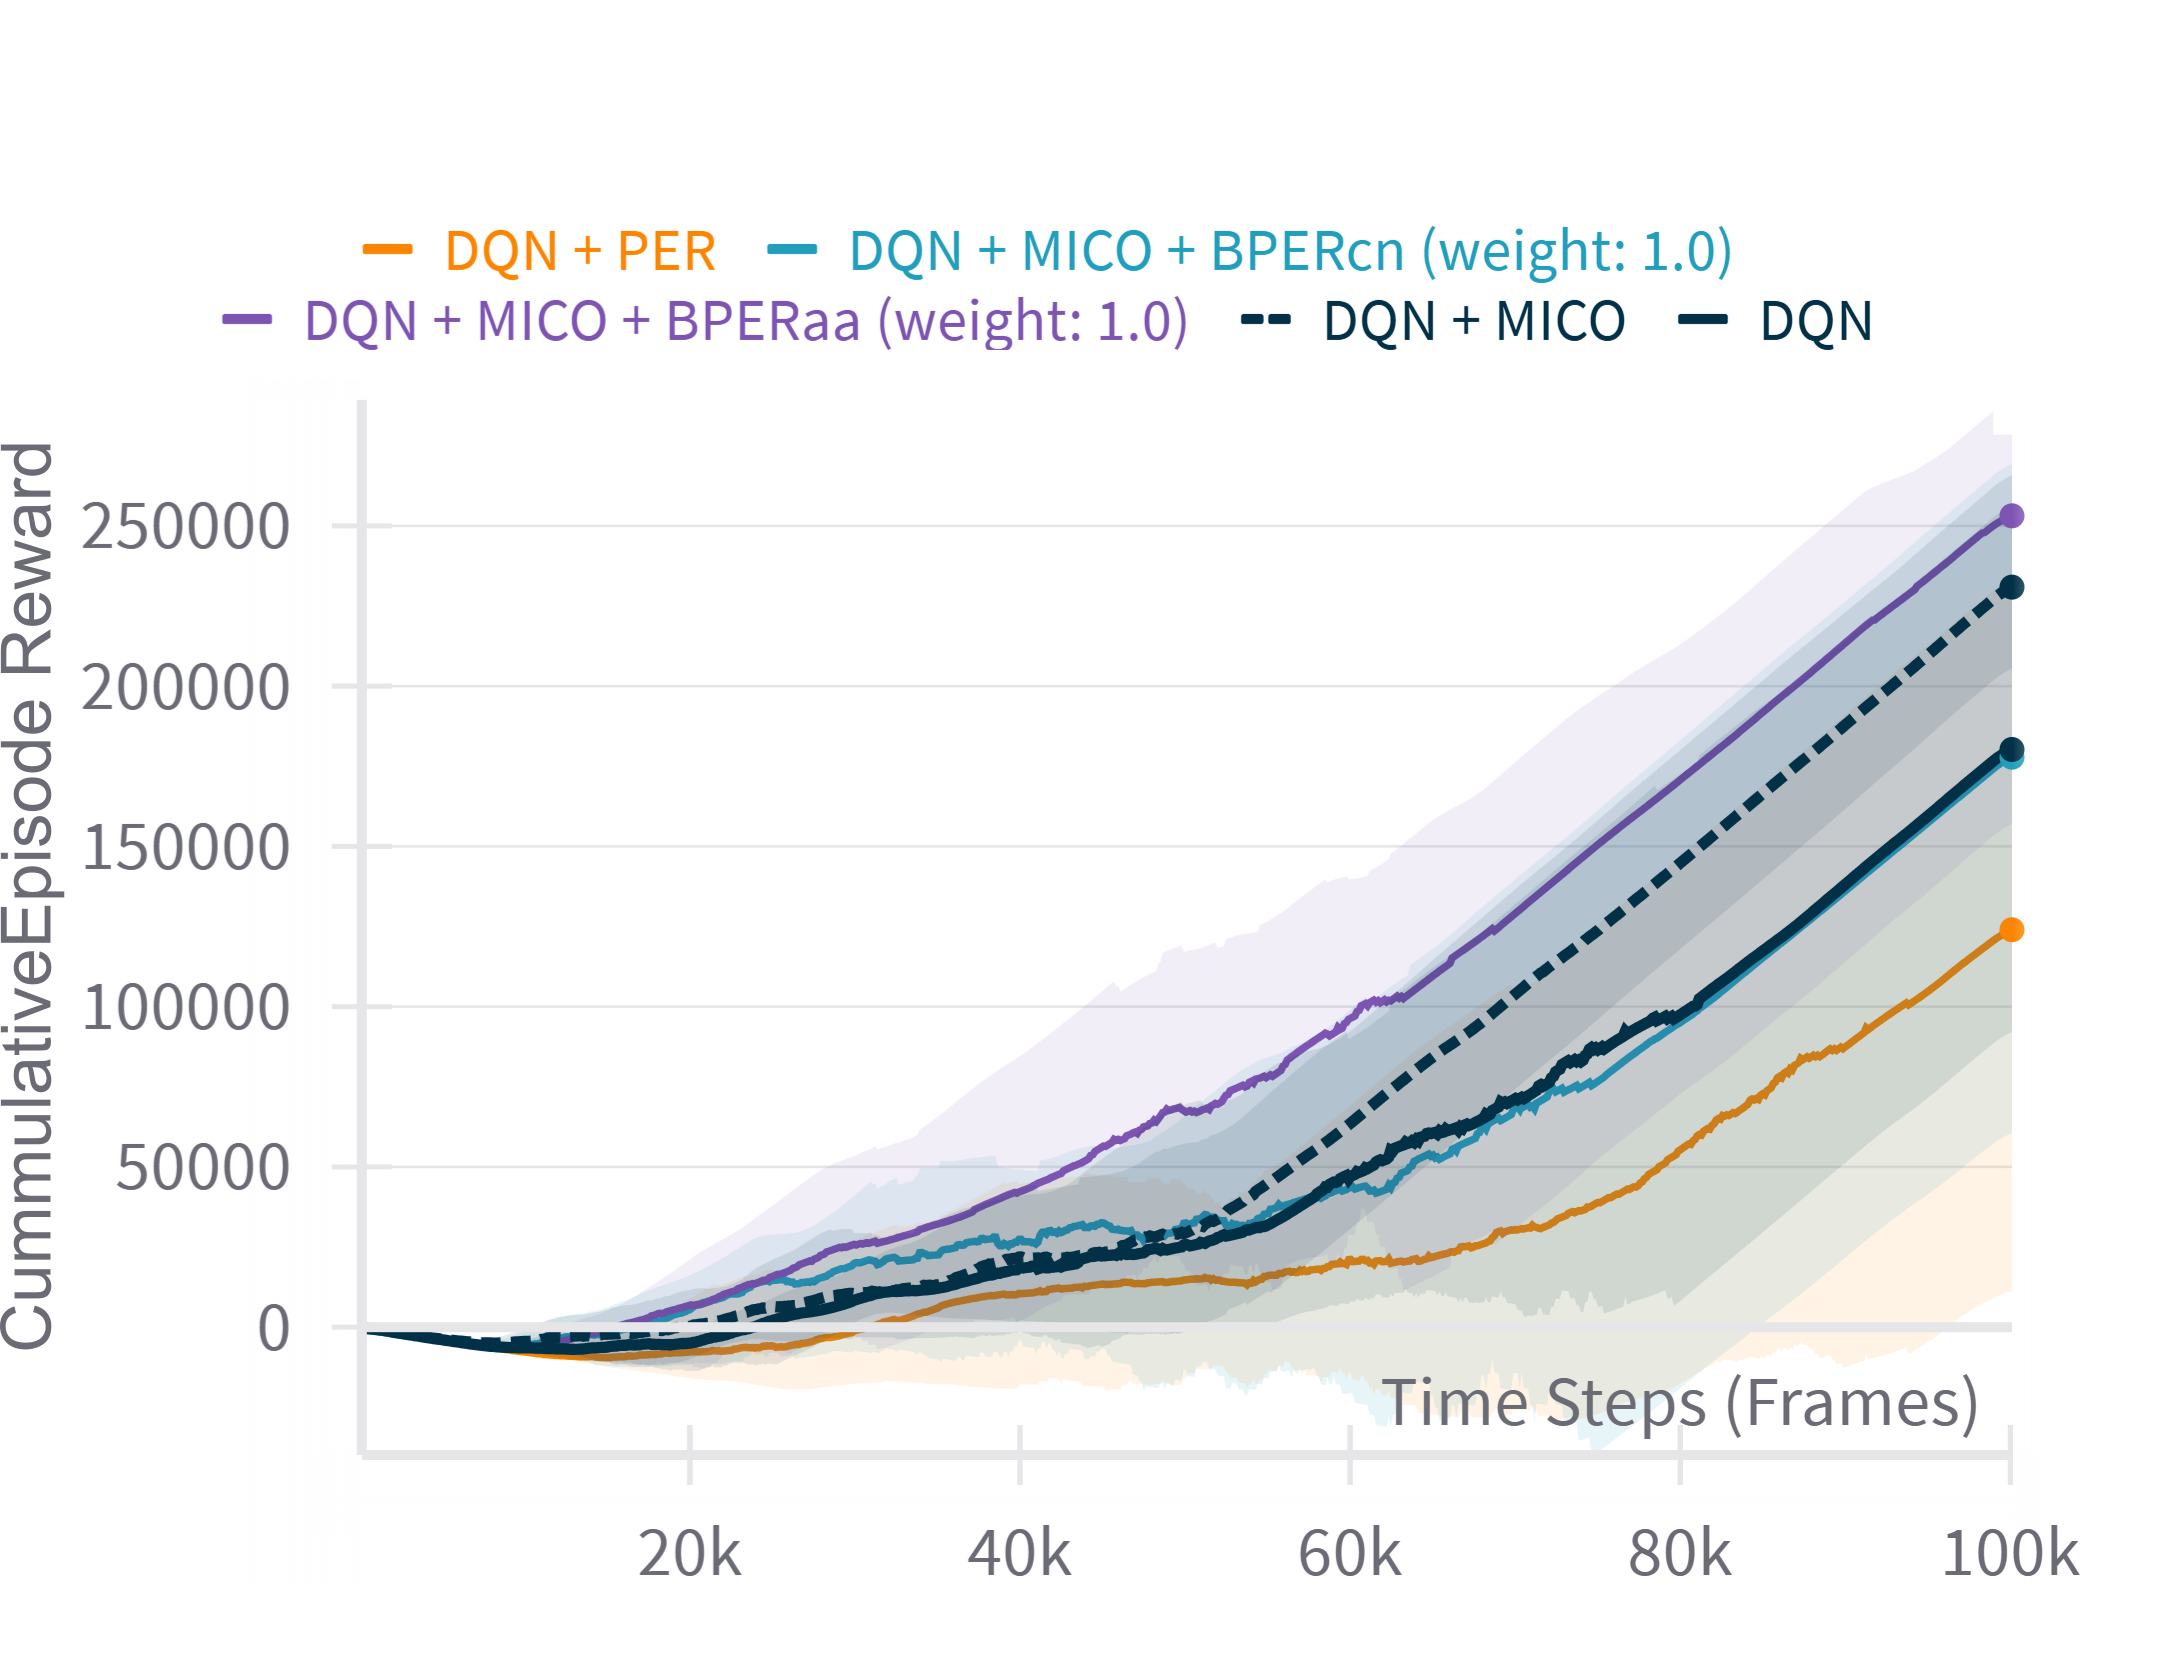
\includegraphics[width=\linewidth]{Results/grid_world/cumulative_episode_return.png}
        \caption{Cumulative Reward}
        \label{fig:cumulative_reward}
    \end{subfigure}
    \caption[Episode and Cumulative Reward]{\textbf{Episode and Cumulative Reward.} Reward performance comparison for different methods over time. The results represent the average from 5 independent executions, with shaded regions indicating the variability for each method.}
    \label{fig:cumulative_episode_reward}

\end{figure}


Exploring other perspective of the previous results, we proposed the episode reward gain to analyze more in detail the level of improvement of the proposed methods against our baselines (DQN and DQN + MICO). Figure \ref{fig:episode_reward_gain_dqn_and_mico} illustrates the Episode Reward gain on two different baselines, calculated on a window of 100 steps, and average over 5 independent executions. It is important to notice that only the mean values were used for the calculations. The results ratifies the excel improvements of BPERaa strategy over the other methods: BPERcn and PER againts both baselines, and showcases similar improvements of both bisimulation strategies in the earlier stages of the training. However, as mentioned before, this performance decreases in BPERcn around the step 30k. Under both baselines, the PER method underperform enormously by hinder the proper learning of the policy.

\begin{figure}[h]
    \centering
    \begin{subfigure}{0.45\textwidth}
    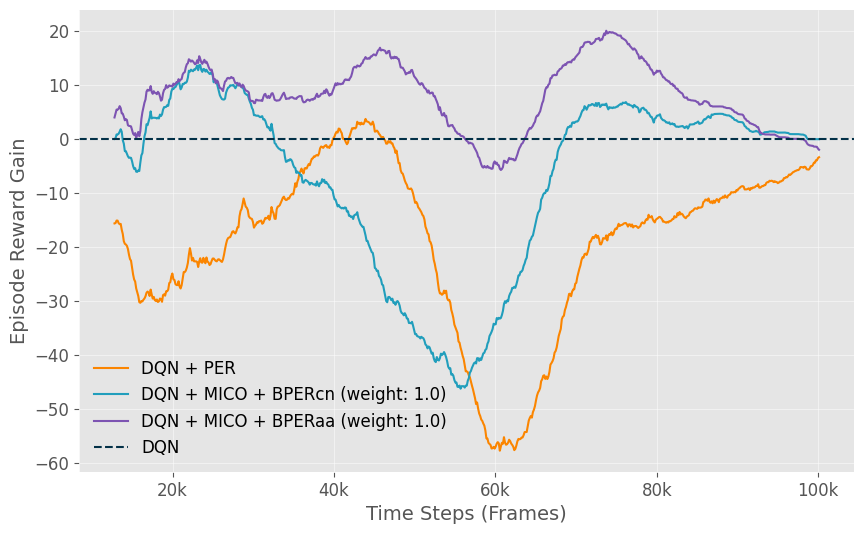
\includegraphics[width=\linewidth]{Results/grid_world/episode_reward_gain_baseline_dqn.png}
        \caption{Baseline DQN}
        \label{fig:episode_reward_gain_dqn}
    \end{subfigure}
    \hfill
    \begin{subfigure}{0.45\textwidth}
        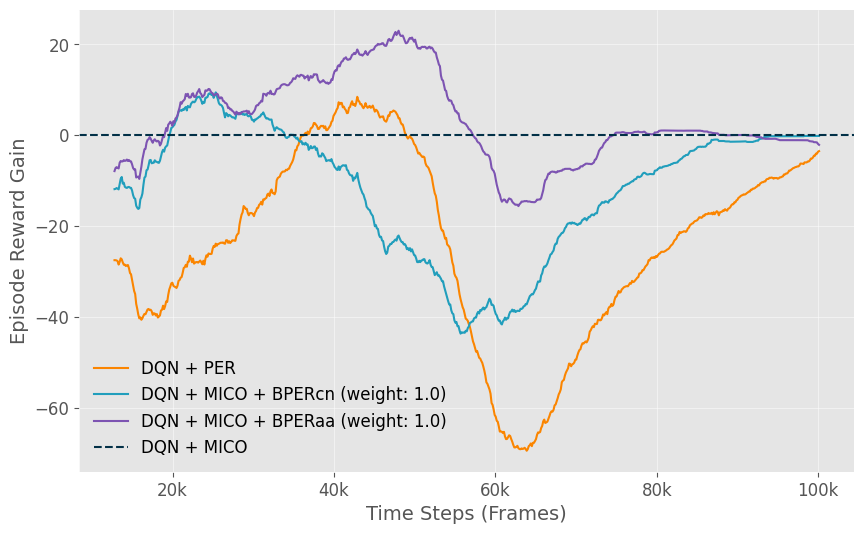
\includegraphics[width=\linewidth]{Results/grid_world/episode_reward_gain_baseline_dqn_mico.png}
        \caption{Baseline DQN + MICO}
        \label{fig:episode_reward_gain_dqn_mico}
    \end{subfigure}
    \caption{Episode Reward Gain }
    \label{fig:episode_reward_gain_dqn_and_mico}
\end{figure}

\section{Task-agnostic Sampling}

In this section, the intention is empirically demonstrate that the proposed method takes into account the behavior for prioritized samples efficiently. To do that, we require a way to quantitatively evaluated how many behavioral dissimilar transitions there are in the current experience replay. Specifically, the on-policy bisimulation recurrent operator $T_K^\pi$ for deterministic environments (see Equation \ref{eq:deterministic_on_policy_bisimulation_metric}) allow us to calculate exact on-policy bisimulation distances. Then, each transition in the experience replay can be associated with a exact bisimulation distance between the current and next state, effectively providing a behavioral value per transition, and allowing us to evaluate the level of behavioral similar or dissimilar transitions in an experience replay. 

Figure \ref{fig:exact_bisimulation_distributions} illustrates the distribution over the exact current-next on-policy bisimulation distances in the experience replay over time. In the strategies BPERcn and BPERaa, the behavioral dissimilar transitions evolve to larger values than PER over time, clearly demonstrating how our method will prioritized more frequently those larger behavioral dissimilar transitions. As the BPERcn encourages highly dissimilar transition between the current and next states approximated in the loop, the results from Figure \ref{fig:exact_bisim_bpercn} are expected. However, a more interesting result is that despite of BPERaa prioritized the transition based on a relative priority to the current mini-batch, this second strategy is still able to prioritize dissimilar experience as efficiently as the strategy BPERcn (see Figure \ref{fig:exact_bisim_bperaa}).

Another interesting result is that even though the method aims to prioritized highlight dissimilar transitions, Figures \ref{fig:exact_bisimulation_distributions} still show a lot of transitions with exact bisimilar distance close to zero, possible coming from the nature of the environment that contains highly similar states.

This result suggest that despite of the td-error is an indicator of possible improvement over the q-values, this is not enough to define a the expected learning improving and in this scenario a notion of behavioral similarity works better as an indicator of expected learning improving.


\begin{figure}[h]
    \centering
    \begin{subfigure}{0.32\textwidth}
    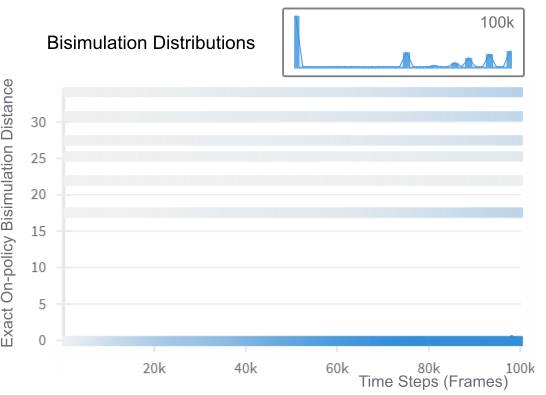
\includegraphics[width=\linewidth]{Results/grid_world/exact_bisimulation_dqn_per.png}
        \caption{DQN + PER}
        \label{fig:exact_bisim_per}
    \end{subfigure}
    \hfill
    \begin{subfigure}{0.32\textwidth}
        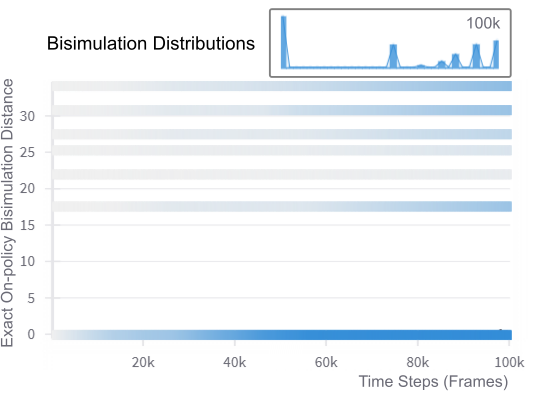
\includegraphics[width=\linewidth]{Results/grid_world/exact_bisimulation_dqn_mico_bpercn.png}
        \caption{DQN (MICO) + BPERcn}
        \label{fig:exact_bisim_bpercn}
    \end{subfigure}
    \hfill
    \begin{subfigure}{0.32\textwidth}
        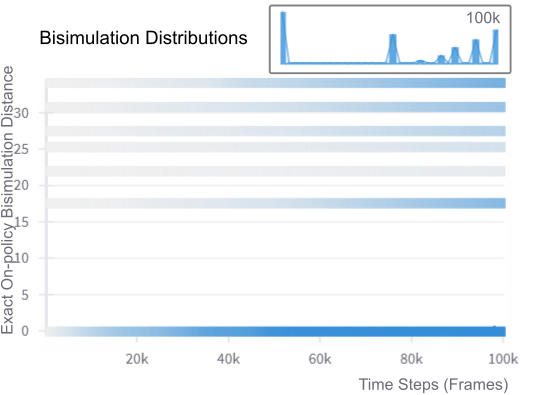
\includegraphics[width=\linewidth]{Results/grid_world/exact_bisimulation_dqn_mico_bperaa.png}
        \caption{DQN (MICO) + BPERaa}
        \label{fig:exact_bisim_bperaa}
    \end{subfigure}
    \caption{Two images side-by-side}
    \label{fig:exact_bisimulation_distributions}
\end{figure}

\begin{figure}[h]
    \centering
    \begin{subfigure}{0.32\textwidth}
    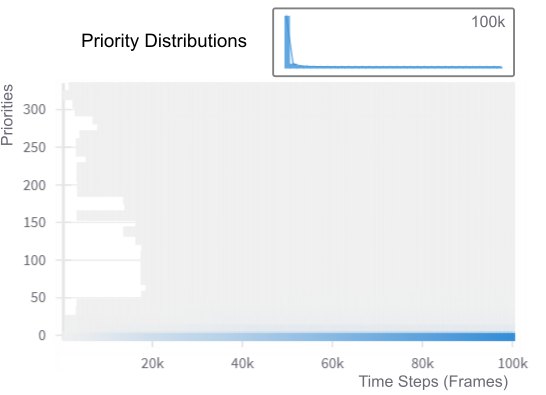
\includegraphics[width=\linewidth]{Results/grid_world/priority_distribution_dqn_per.png}
        \caption{DQN + PER}
        \label{fig:on_policy_weighting}
    \end{subfigure}
    \hfill
    \begin{subfigure}{0.32\textwidth}
        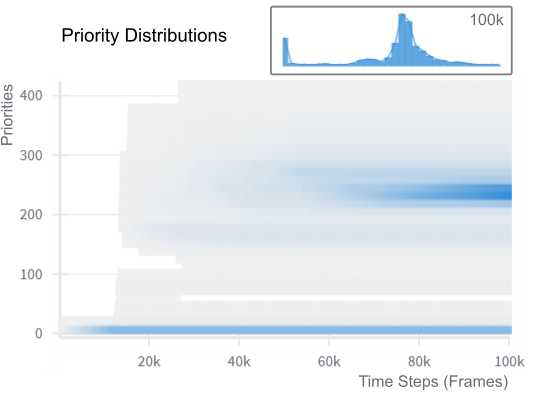
\includegraphics[width=\linewidth]{Results/grid_world/priority_distribution_dqn_mico_bpercn.png}
        \caption{DQN (MICO) + BPERcn}
        \label{fig:uniform_weighting}
    \end{subfigure}
    \hfill
    \begin{subfigure}{0.32\textwidth}
        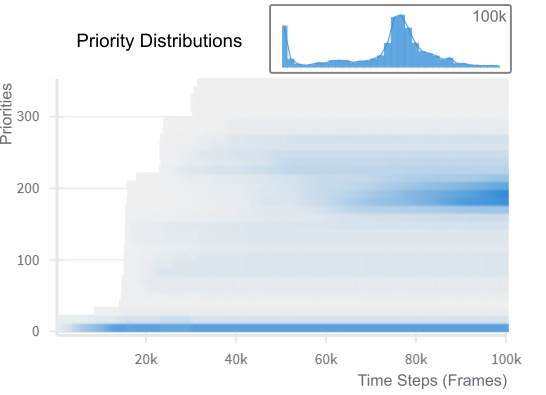
\includegraphics[width=\linewidth]{Results/grid_world/priority_distribution_dqn_mico_bperaa.png}
        \caption{DQN (MICO) + BPERaa}
        \label{fig:uniform_weighting}
    \end{subfigure}
    \caption{Two images side-by-side}
    \label{fig:outdated_priorities}
\end{figure}



\begin{figure}[h]
    \centering
    \begin{subfigure}{1.\textwidth}
    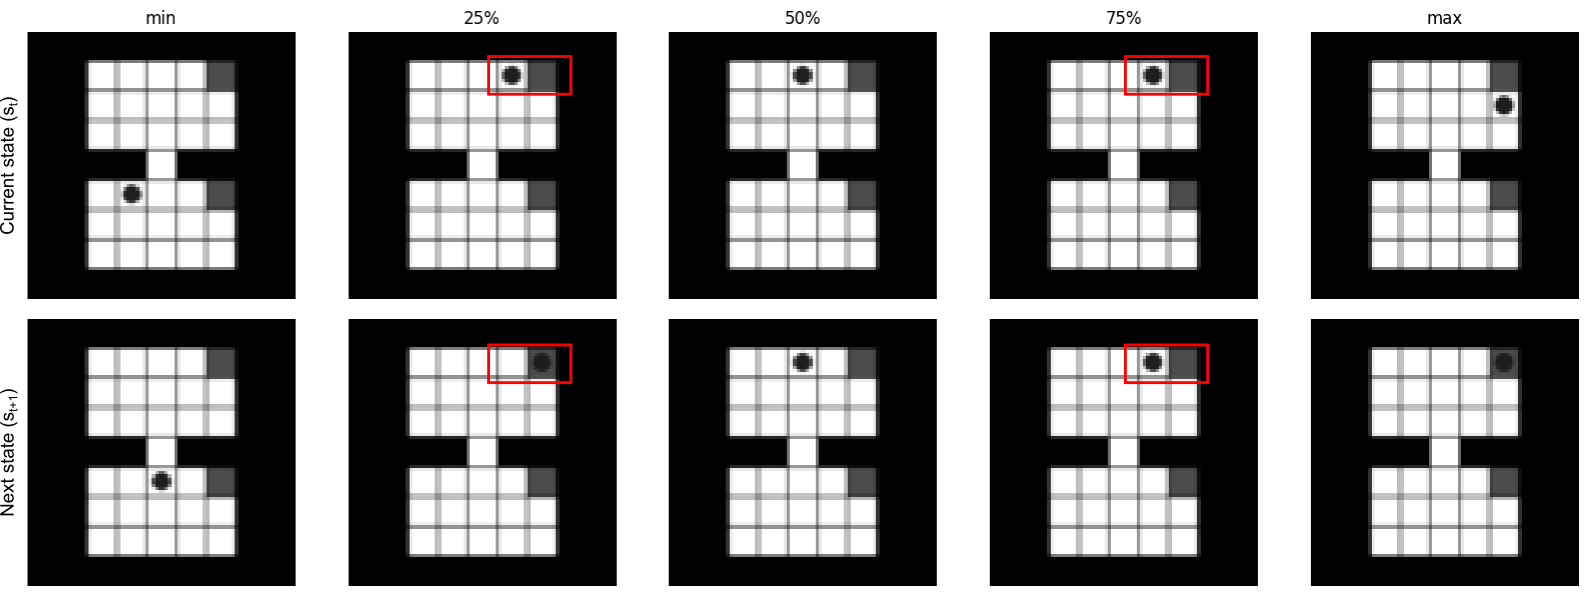
\includegraphics[width=\linewidth]{Results/grid_world/quartiles_images_per.png}
        \caption{DQN + PER}
        \label{fig:on_policy_weighting}
    \end{subfigure}
    \hfill
    \begin{subfigure}{1.\textwidth}
        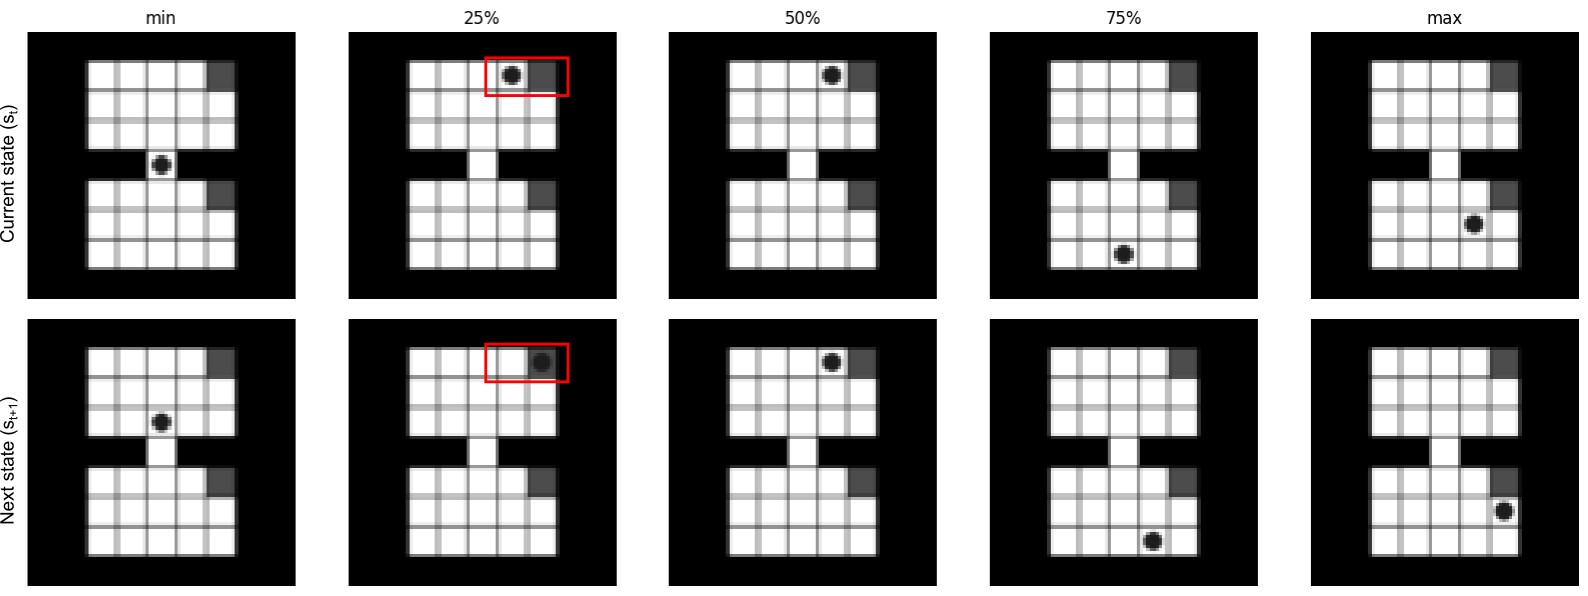
\includegraphics[width=\linewidth]{Results/grid_world/quartiles_images_dqn_mico_bpercn.png}
        \caption{DQN (MICO) + BPERcn}
        \label{fig:uniform_weighting}
    \end{subfigure}
    \hfill
    \begin{subfigure}{1.\textwidth}
        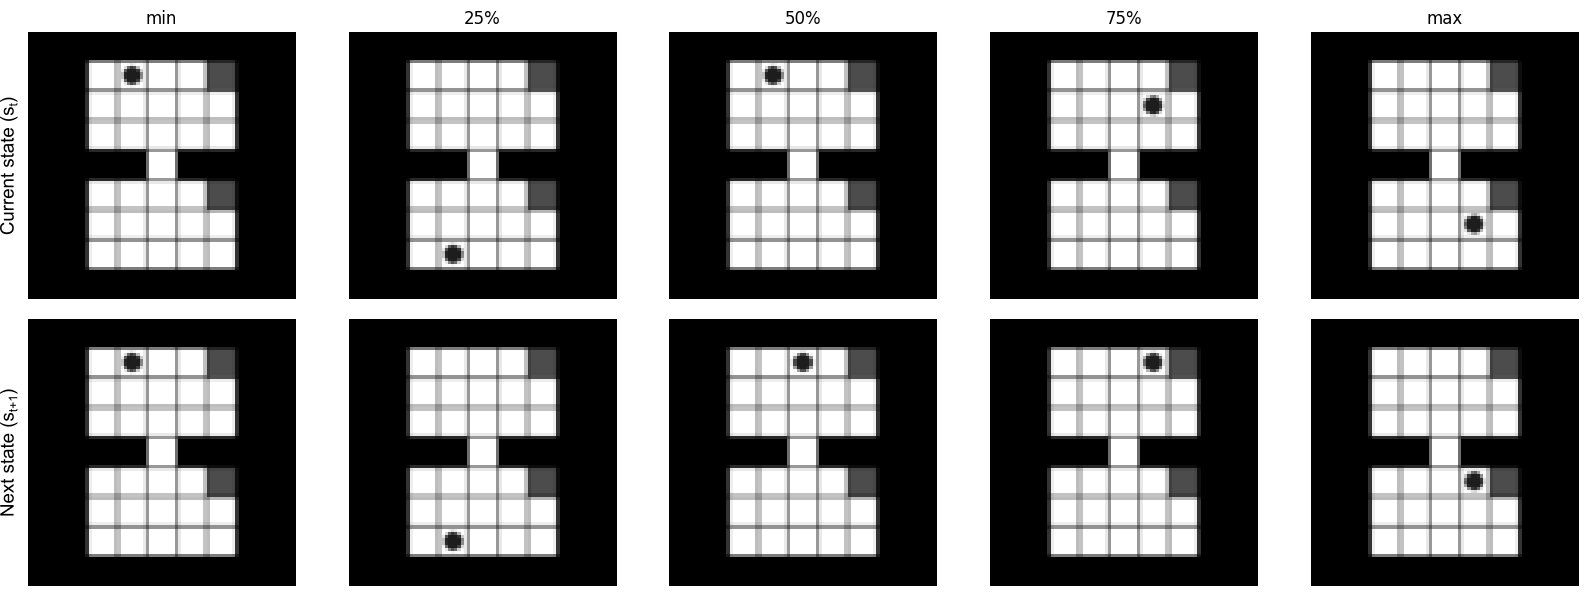
\includegraphics[width=\linewidth]{Results/grid_world/quartiles_images_dqn_mico_bperaa.png}
        \caption{DQN (MICO) + BPERaa}
        \label{fig:uniform_weighting}
    \end{subfigure}
    \caption{Two images side-by-side}
    \label{fig:outdated_priorities}
\end{figure}


\section{Outdated Priorities}

\begin{figure}[h]
    \centering
    \begin{subfigure}{0.45\textwidth}
    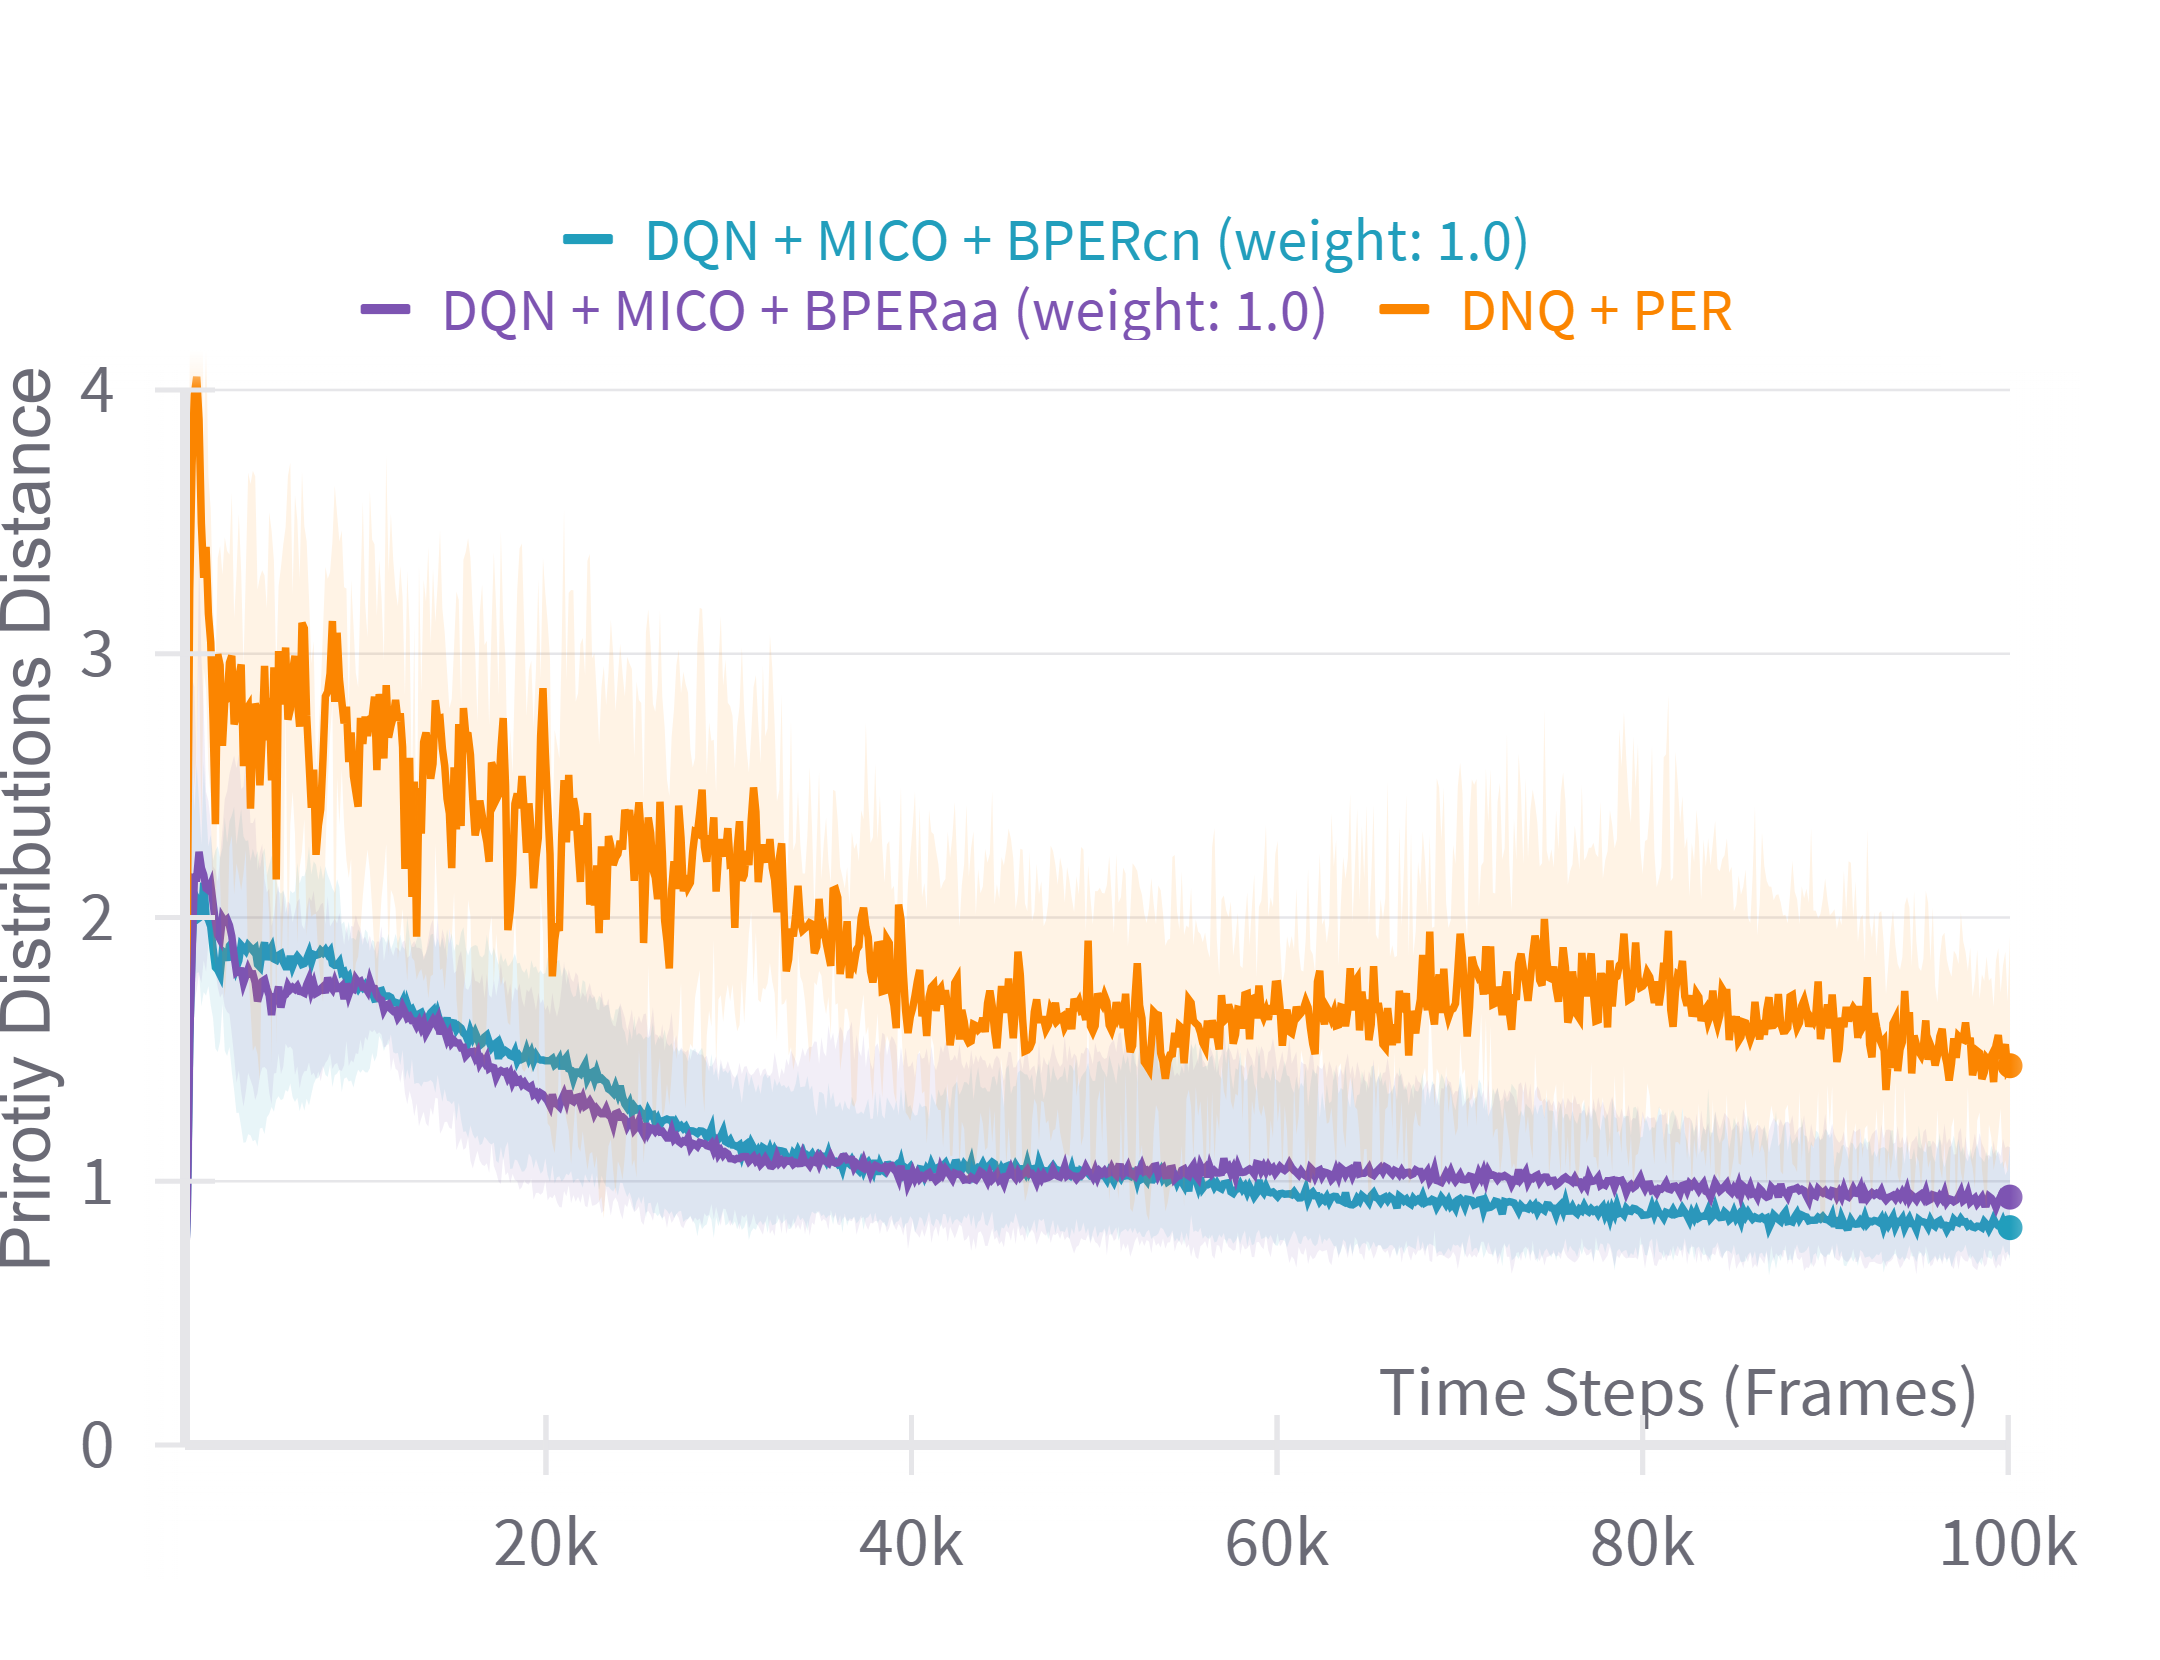
\includegraphics[width=\linewidth]{Results/grid_world/on_policy_weighting_outdated_priorities.png}
        \caption{On-policy Weighting}
        \label{fig:on_policy_weighting}
    \end{subfigure}
    \hfill
    \begin{subfigure}{0.45\textwidth}
        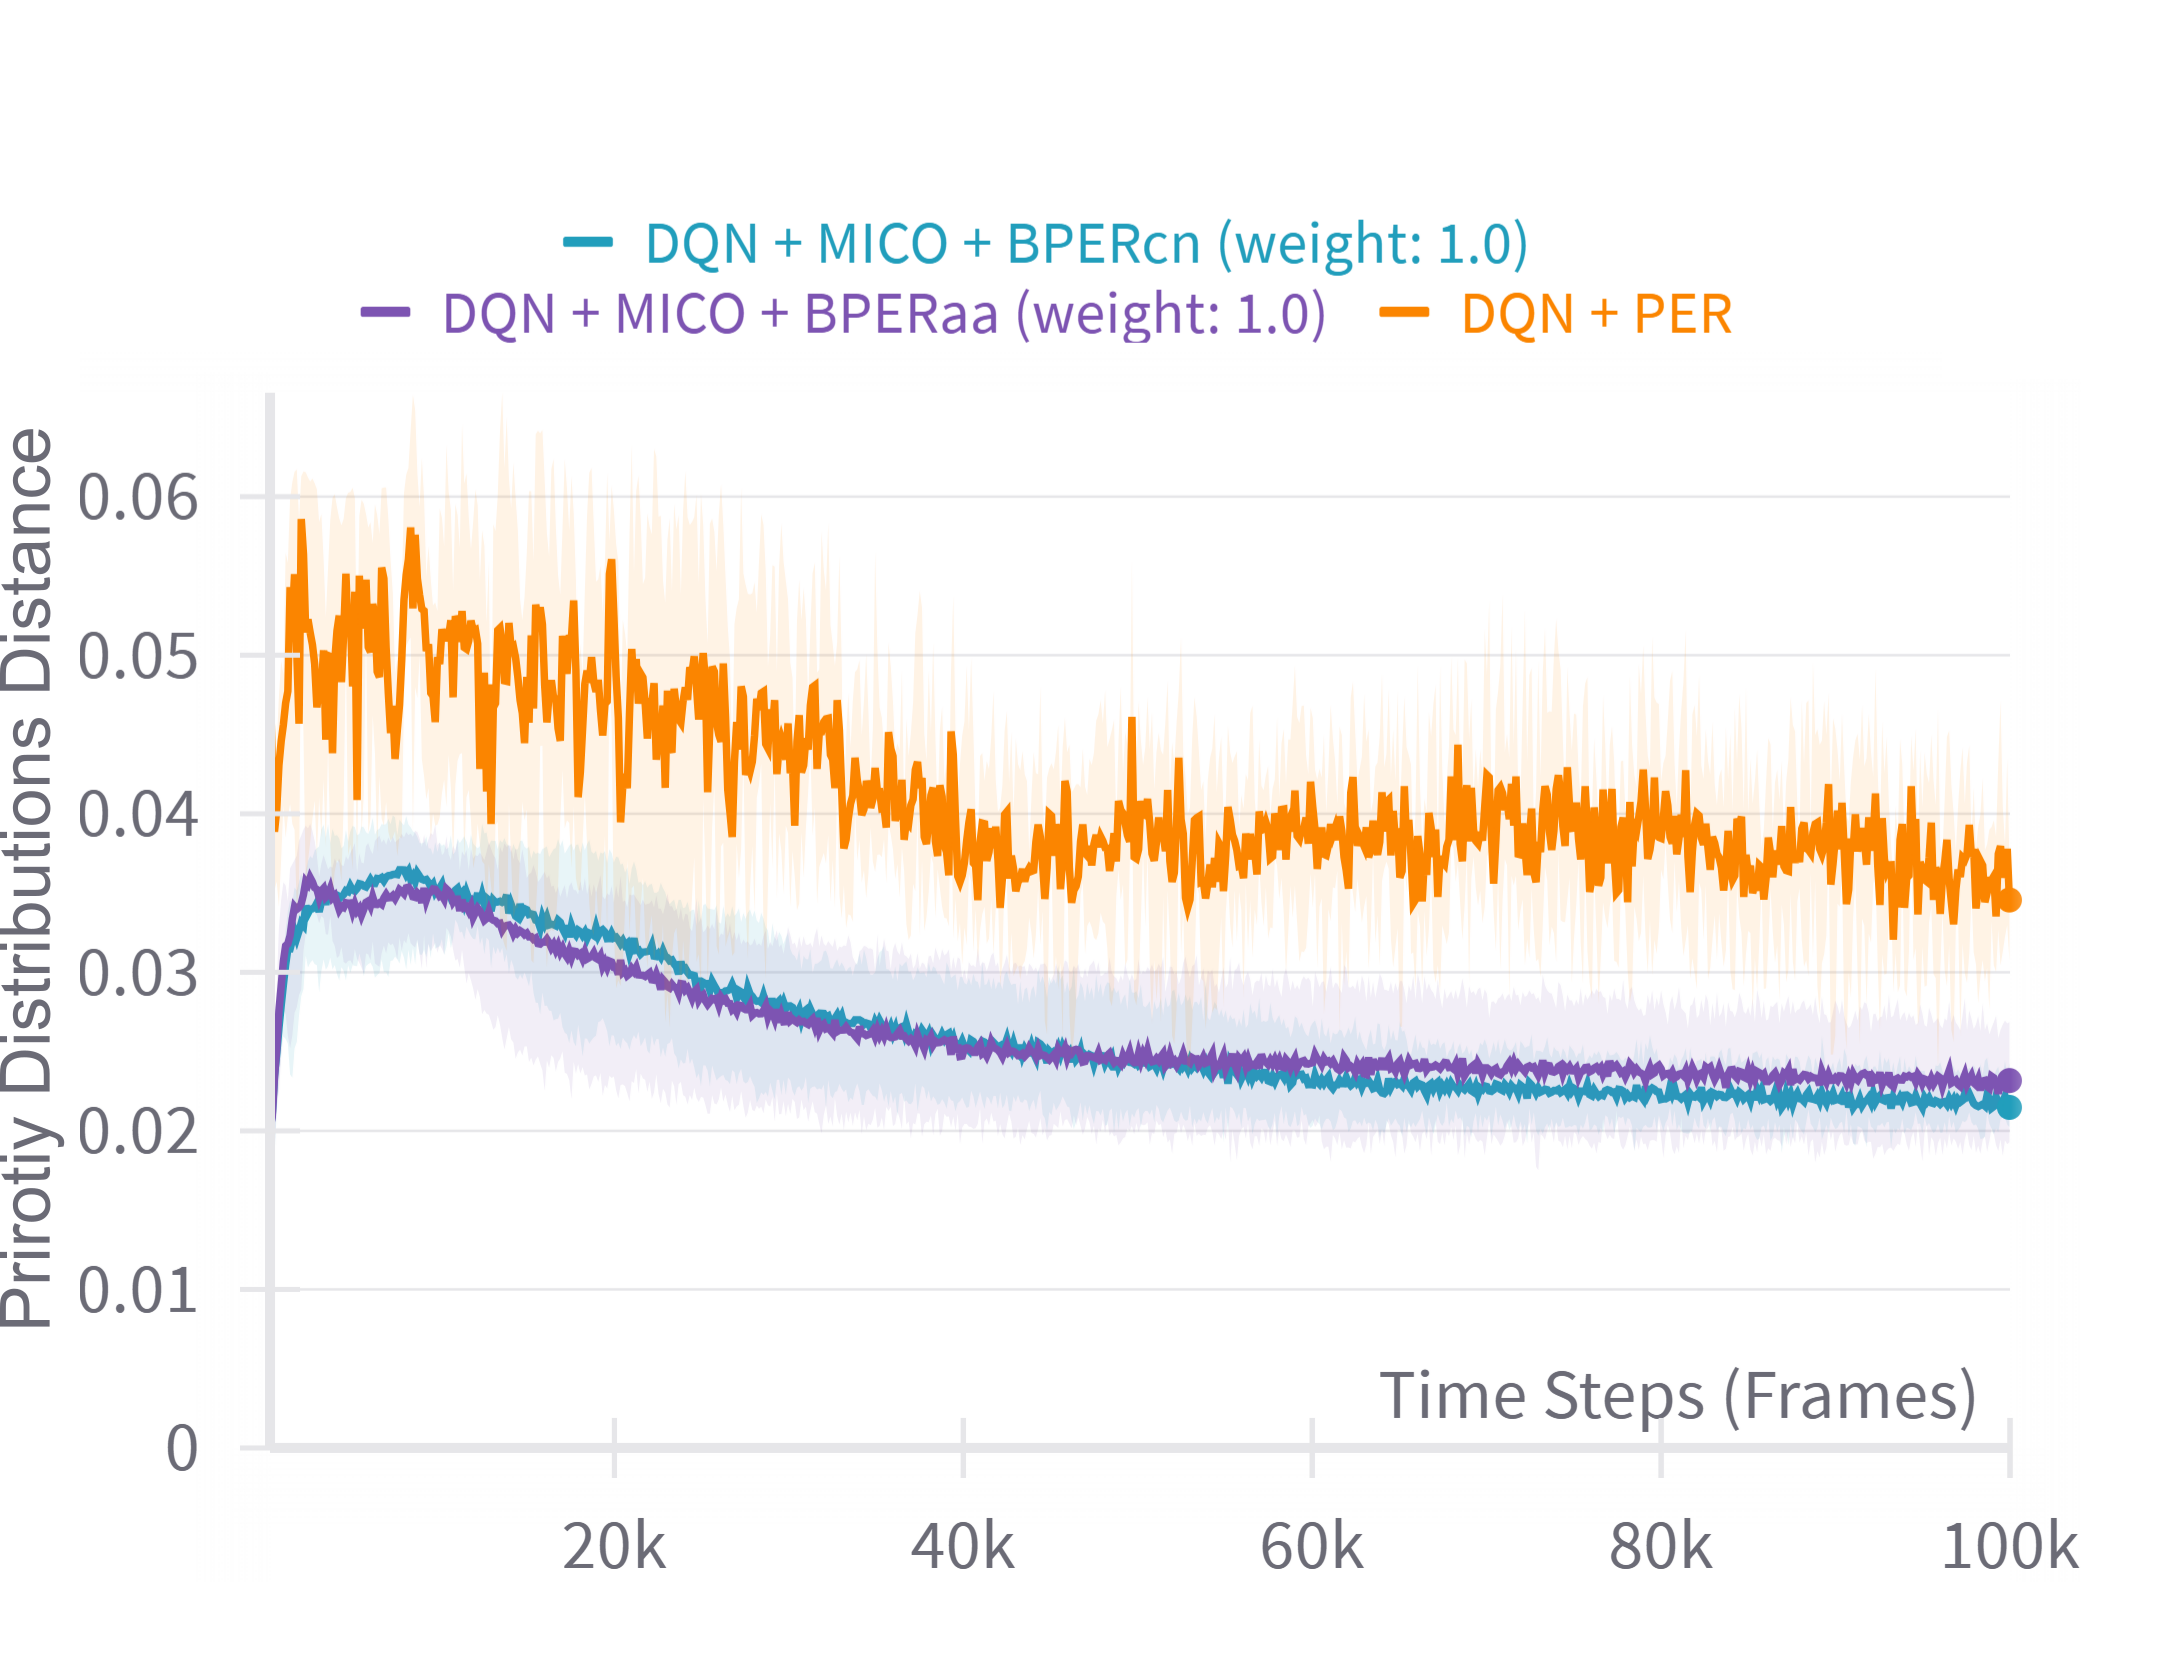
\includegraphics[width=\linewidth]{Results/grid_world/uniform_weighting_outdated_priorities.png}
        \caption{Uniform Weighting}
        \label{fig:uniform_weighting}
    \end{subfigure}
    \caption{Two images side-by-side}
    \label{fig:outdated_priorities}
\end{figure}



\section{State Space Coverage}

\begin{figure}[h]
    \centering
    % Add horizontal space to center the first two subfigures
    \hspace*{\fill}
    \begin{subfigure}{0.45\textwidth}
        \centering % Center the individual subfigure
        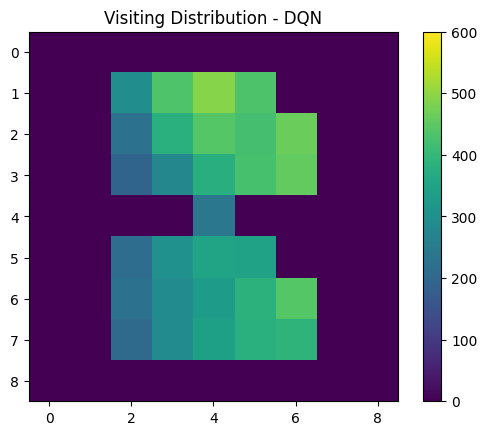
\includegraphics[width=0.70\linewidth]{Results/grid_world/visitation_distribution_dqn.png}
        \caption{DQN}
        \label{fig:on_policy_weighting}
    \end{subfigure}
    \hspace*{\fill} % Adjust space between subfigures
    \begin{subfigure}{0.45\textwidth}
        \centering % Center the individual subfigure
        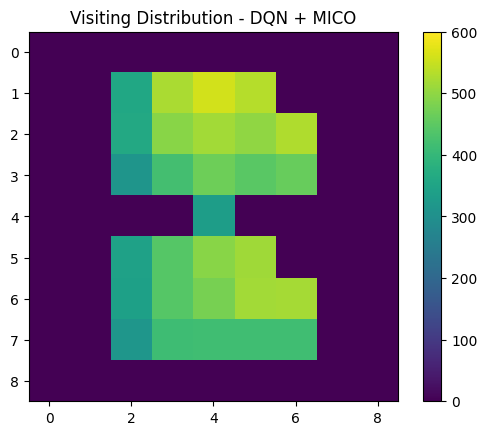
\includegraphics[width=0.70\linewidth]{Results/grid_world/visitation_distribution_dqn_mico.png}
        \caption{DQN + MICO}
        \label{fig:uniform_weighting}
    \end{subfigure}
    \hspace*{\fill} % Add horizontal space to center the first two subfigures
    \vfill
    \begin{subfigure}{0.32\textwidth}
        \centering
        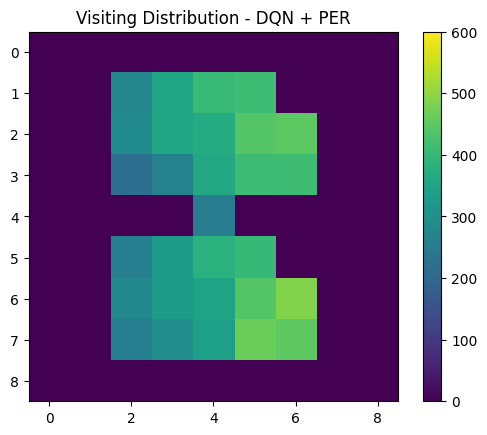
\includegraphics[width=\linewidth]{Results/grid_world/visitation_distribution_dqn_per.png}
        \caption{DQN + PER}
        \label{fig:uniform_weighting_2}
    \end{subfigure}
    \hfill
    \begin{subfigure}{0.32\textwidth}
        \centering
        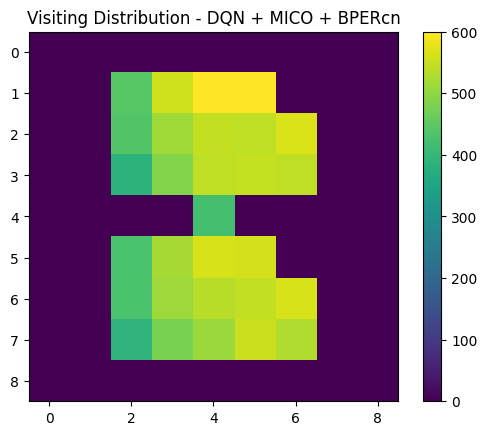
\includegraphics[width=\linewidth]{Results/grid_world/visitation_distribution_dqn_mico_bpercn.png}
        \caption{DQN + MICO + BPERcn}
        \label{fig:uniform_weighting_3}
    \end{subfigure}
    \hfill
    \begin{subfigure}{0.32\textwidth}
        \centering
        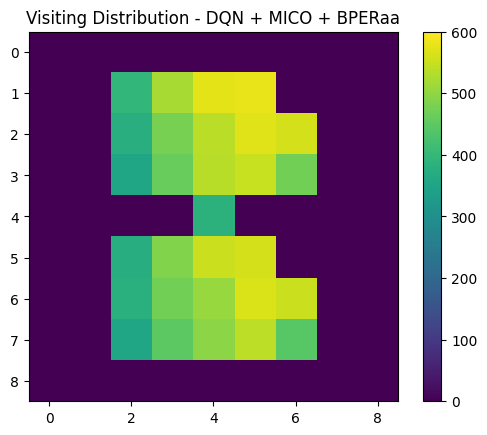
\includegraphics[width=\linewidth]{Results/grid_world/visitation_distribution_dqn_mico_bperaa.png}
        \caption{DQN + MICO + BPERaa}
        \label{fig:uniform_weighting_4}
    \end{subfigure}
    \caption{Two images side-by-side}
    \label{fig:outdated_priorities}
\end{figure}


\begin{figure}
    \centering
    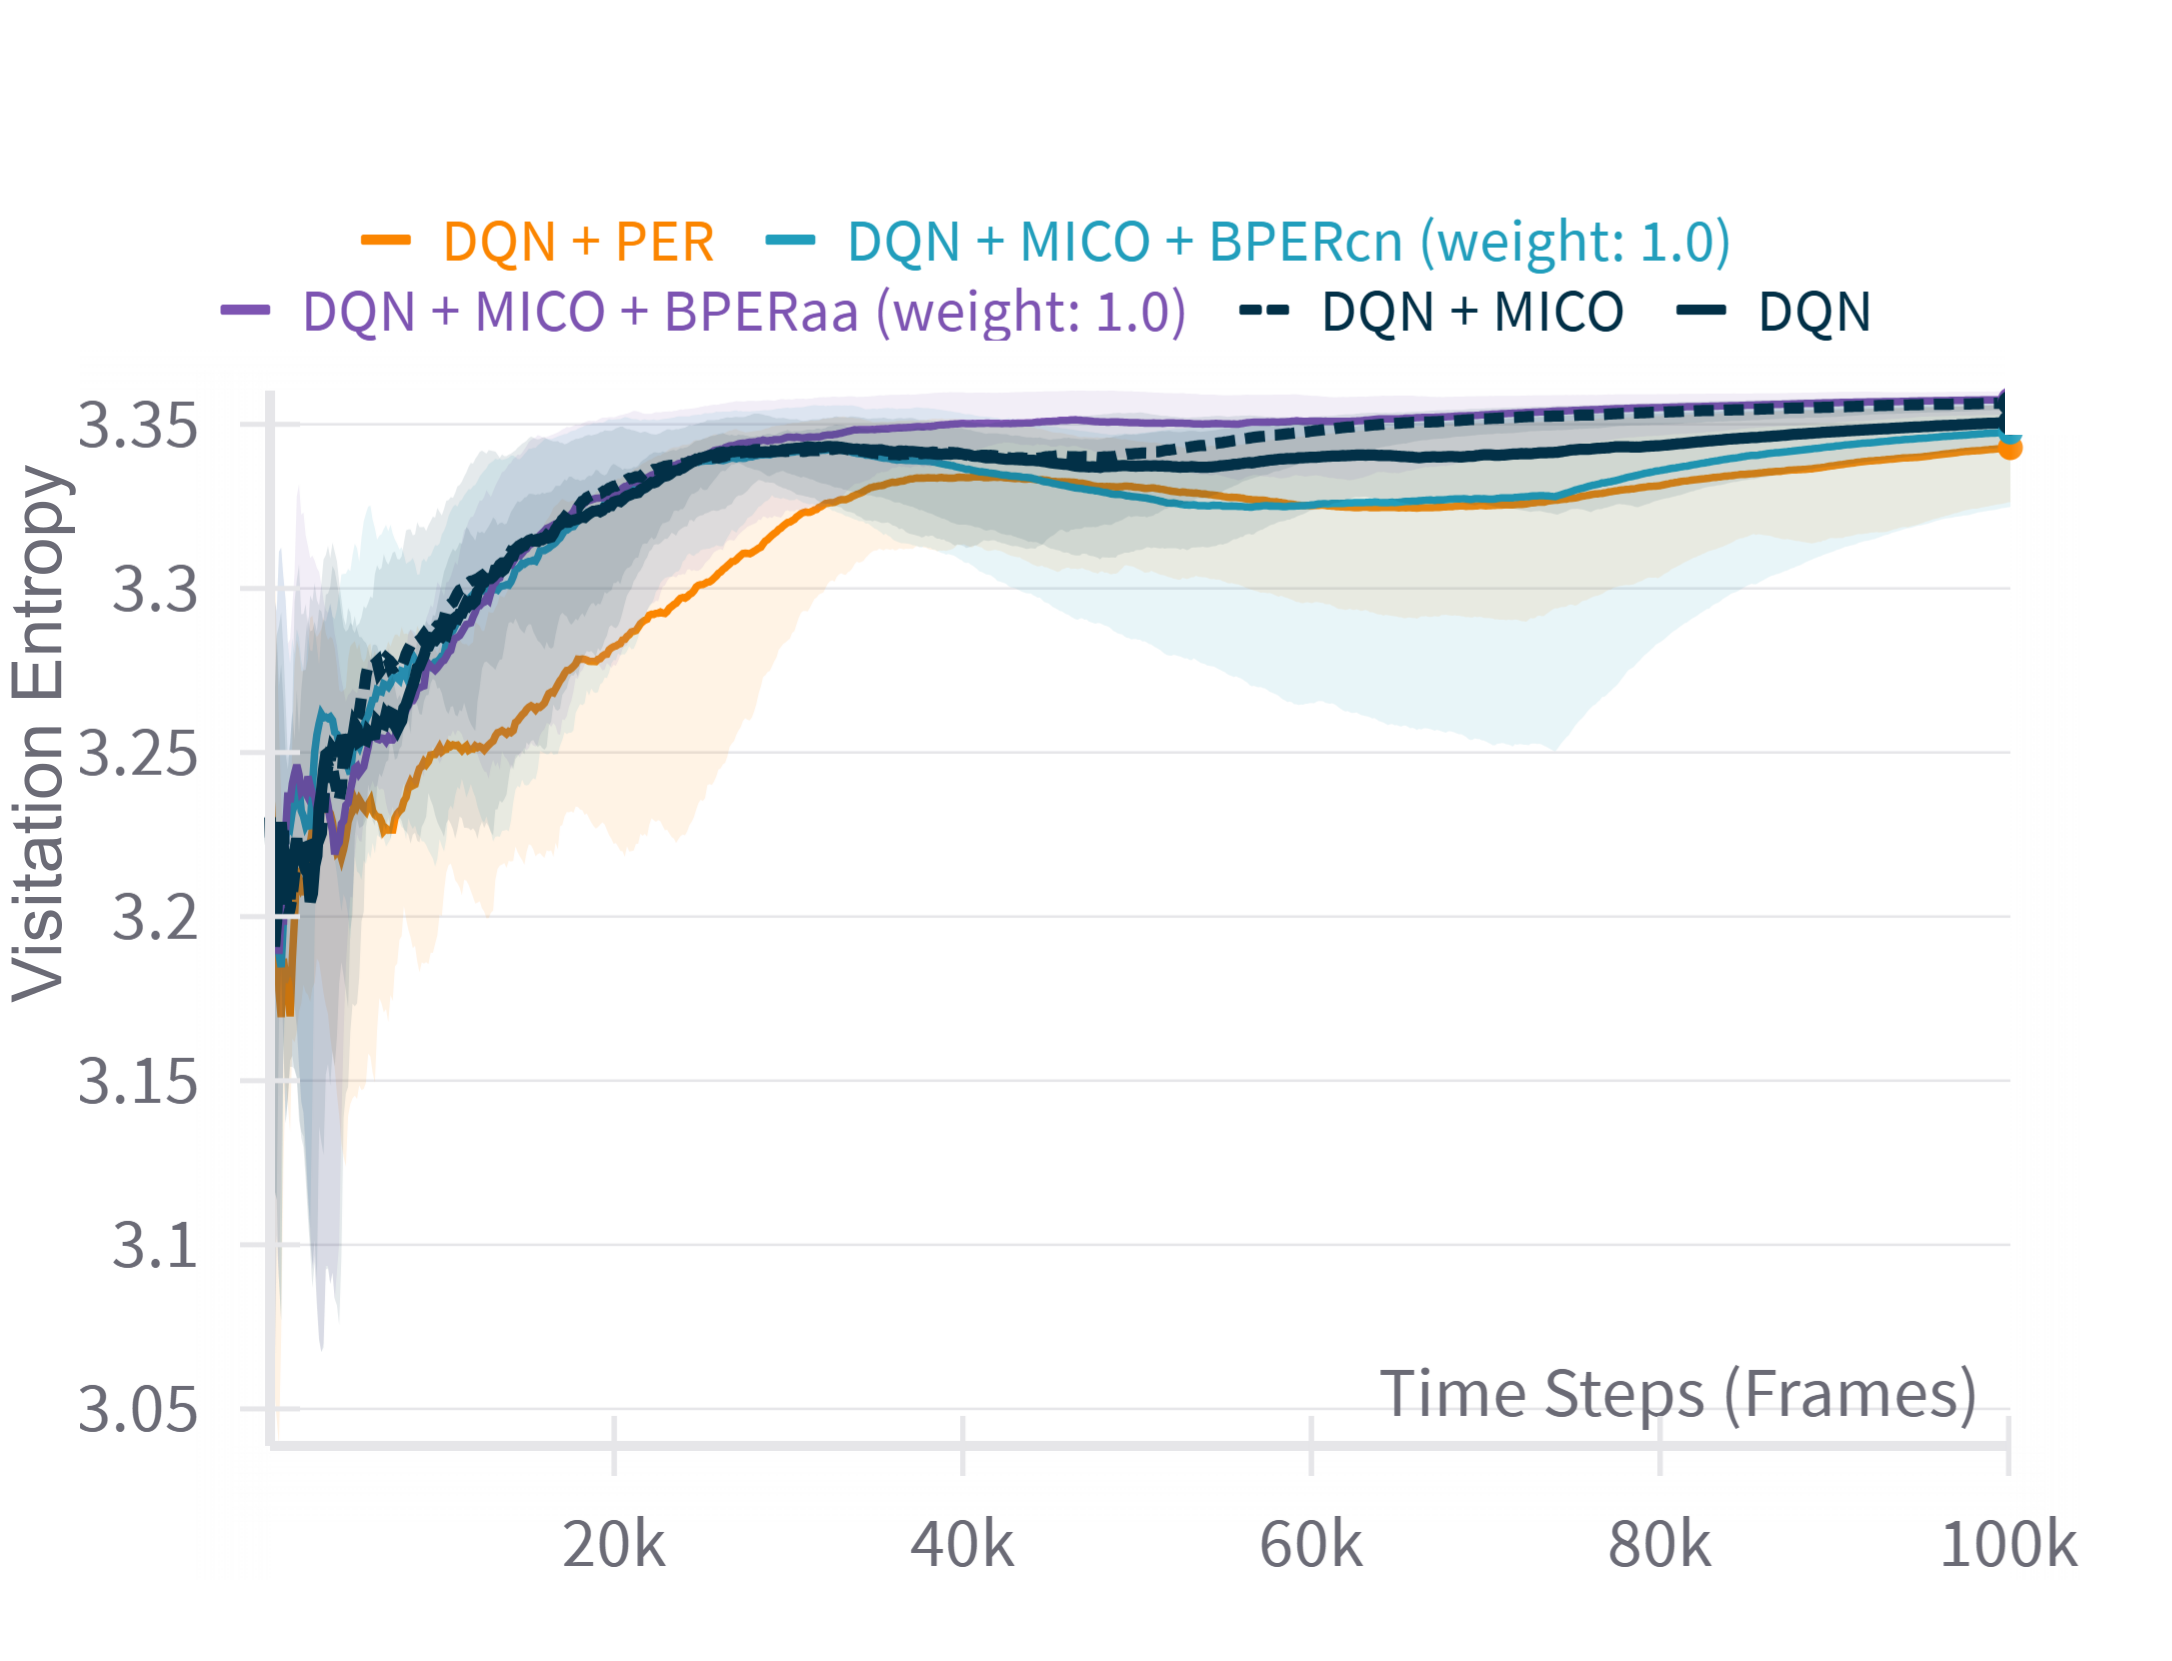
\includegraphics[width=1.\linewidth]{Results/grid_world/state_visitation_entropy.png}
    \caption{Caption}
    \label{fig:enter-label}
\end{figure}


\section{General RL Performance}


\begin{figure}[h]
    \centering
    \begin{subfigure}{0.45\textwidth}
    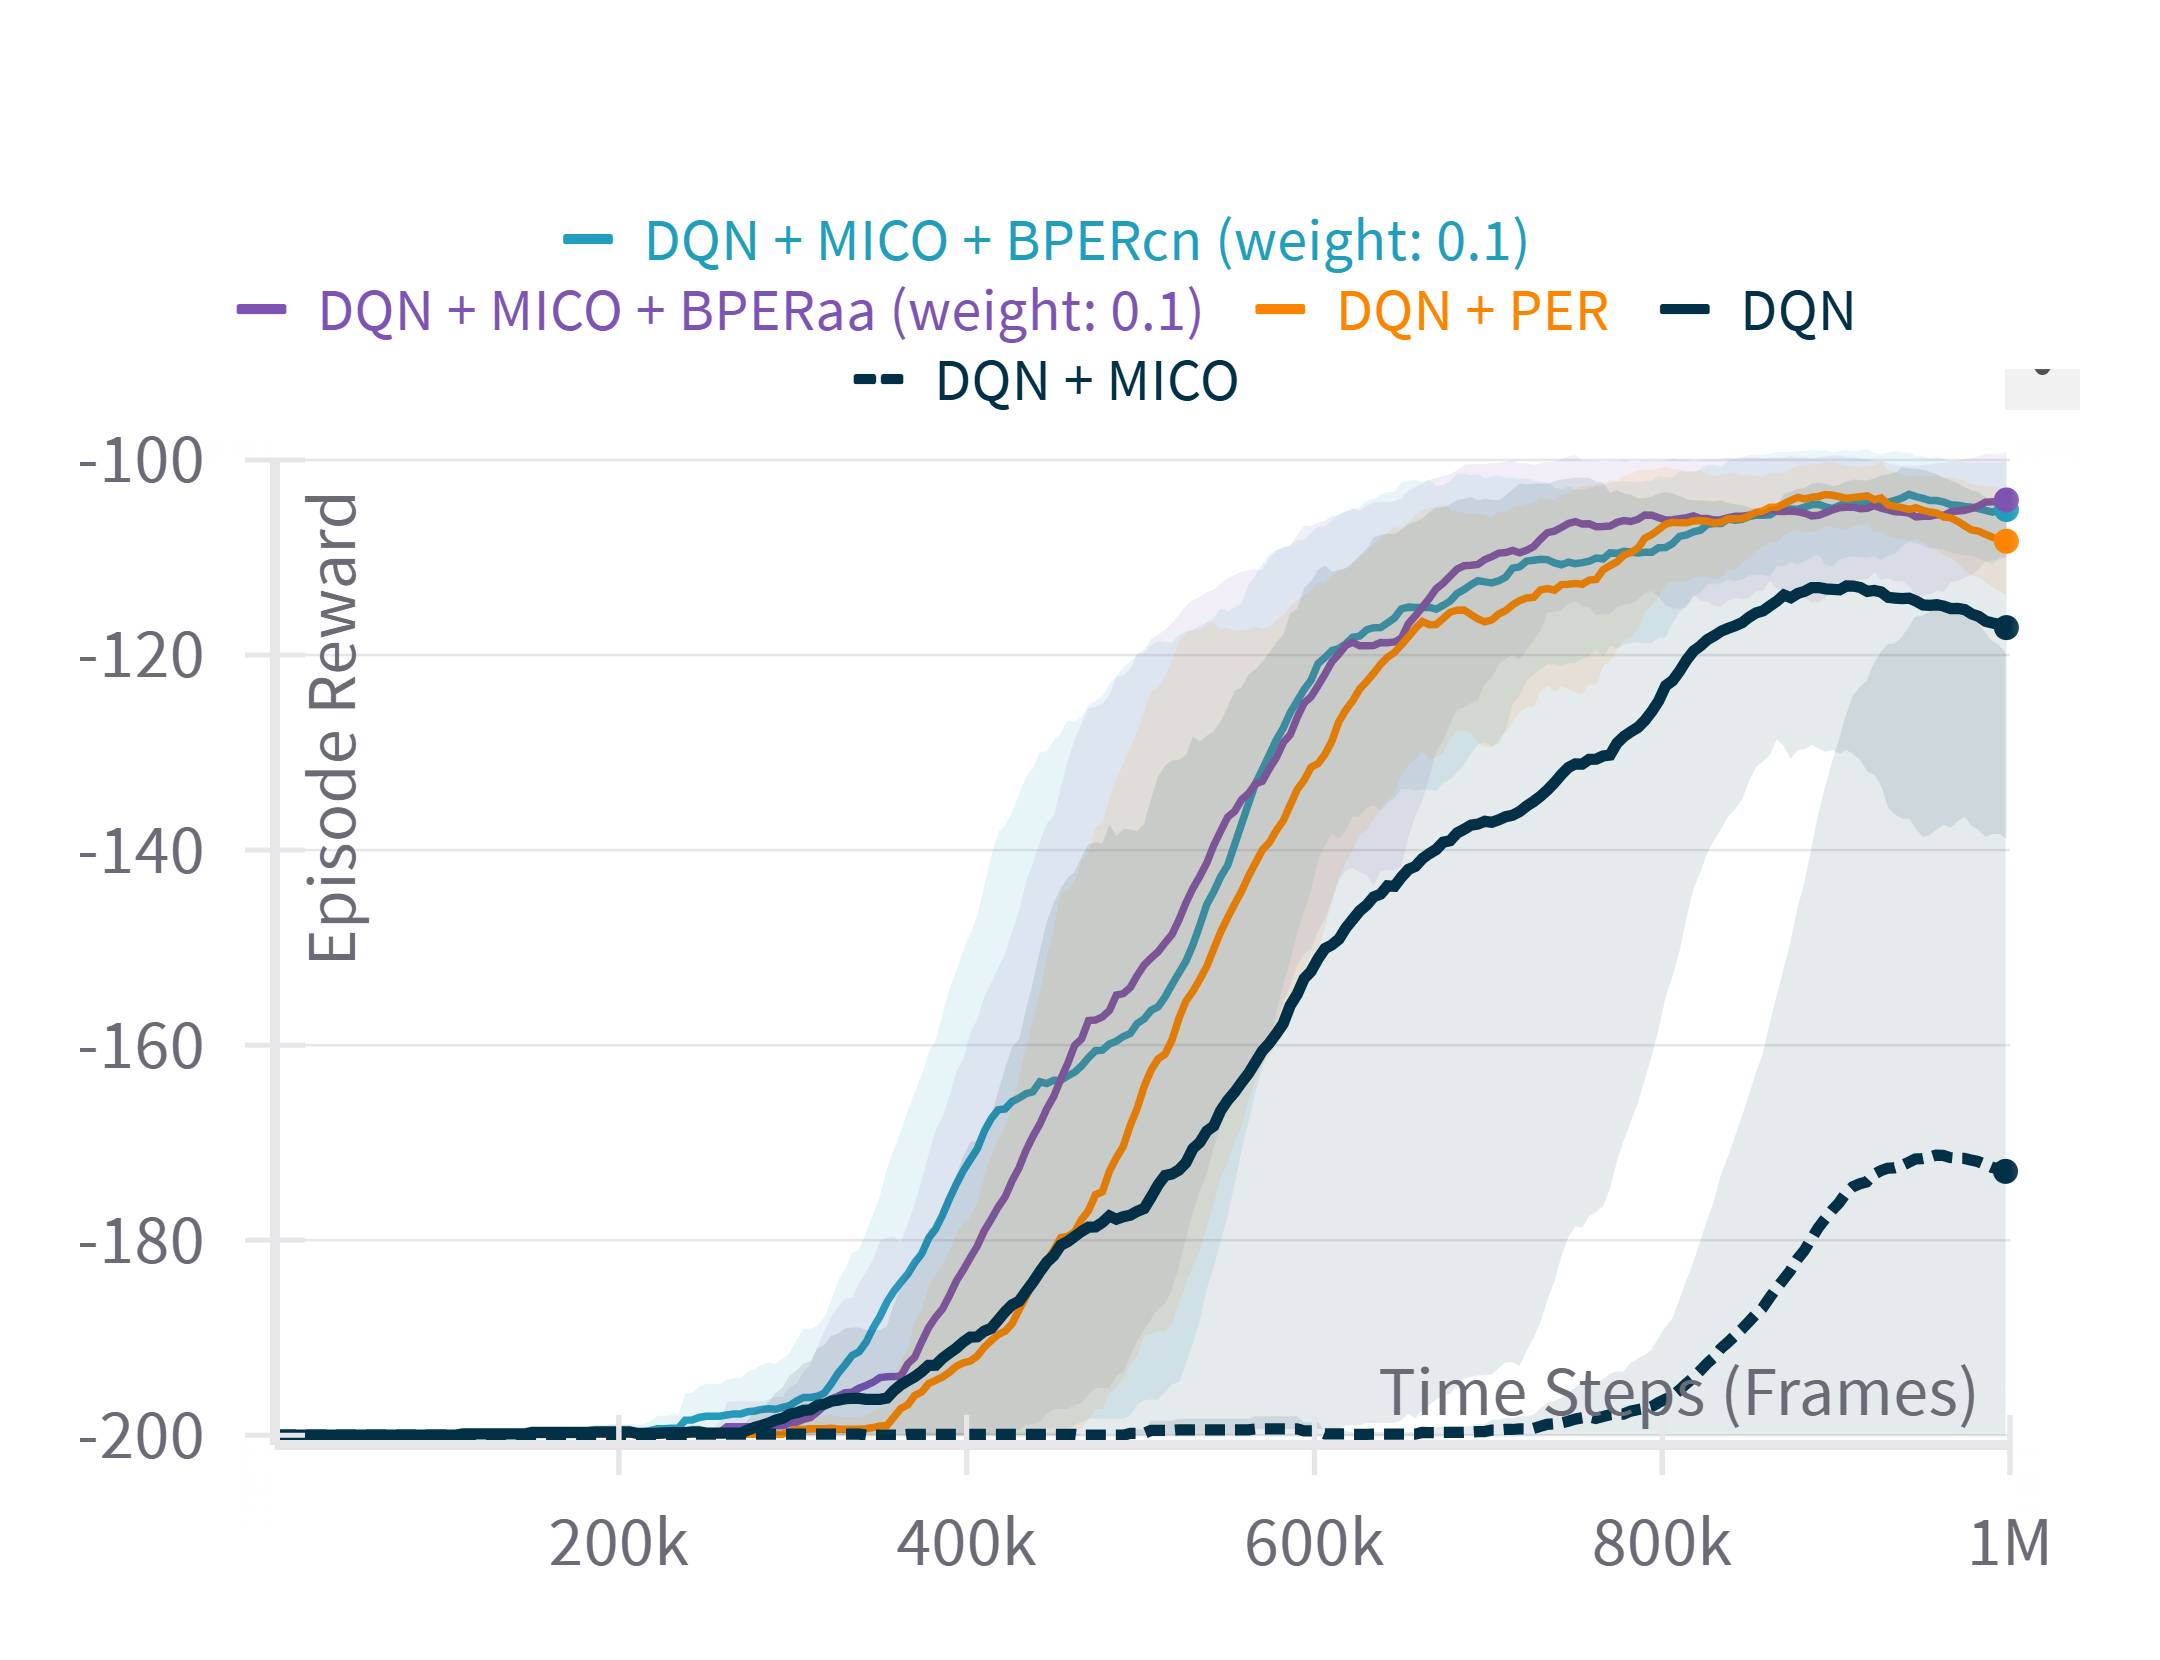
\includegraphics[width=\linewidth]{Results/general_results/episode_reward_mountaincarv0.png}
        \caption{MountainCar-v0}
        \label{fig:on_policy_weighting}
    \end{subfigure}
    \hfill
    \begin{subfigure}{0.45\textwidth}
        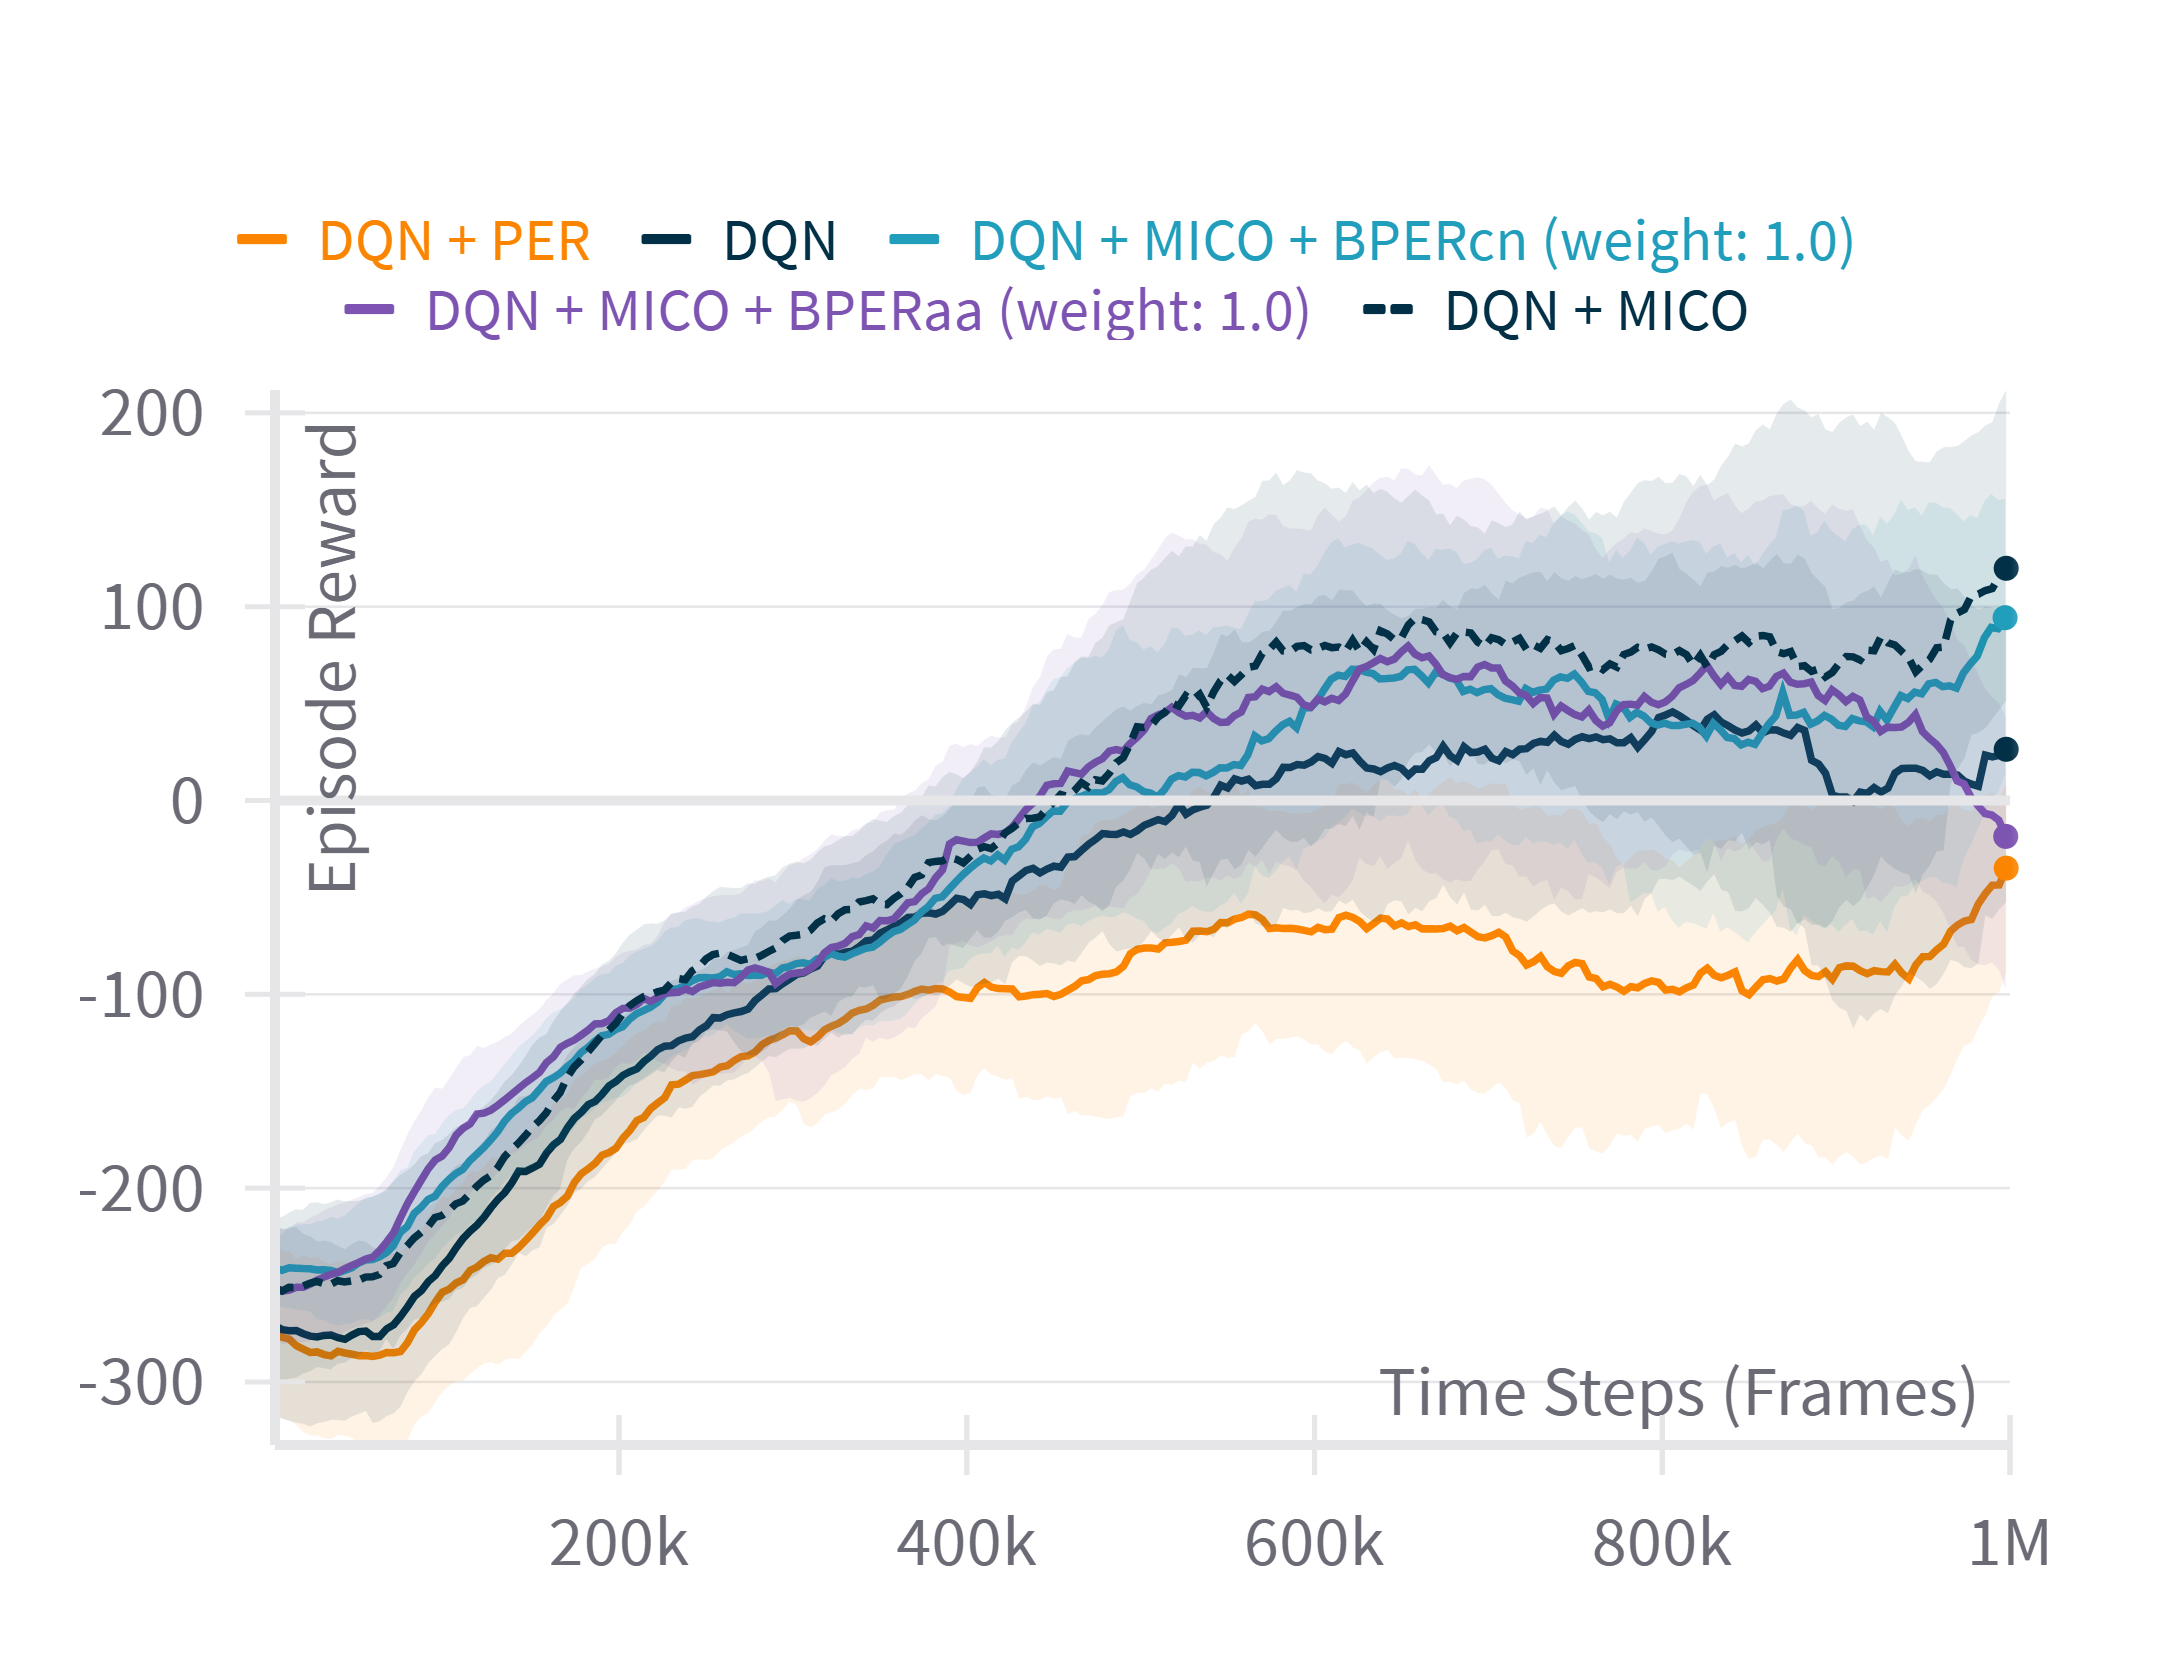
\includegraphics[width=\linewidth]{Results/general_results/episode_reward_lunarlander.png}
        \caption{LunarLander-v1}
        \label{fig:uniform_weighting}
    \end{subfigure}
    \hfill
    \begin{subfigure}{0.45\textwidth}
        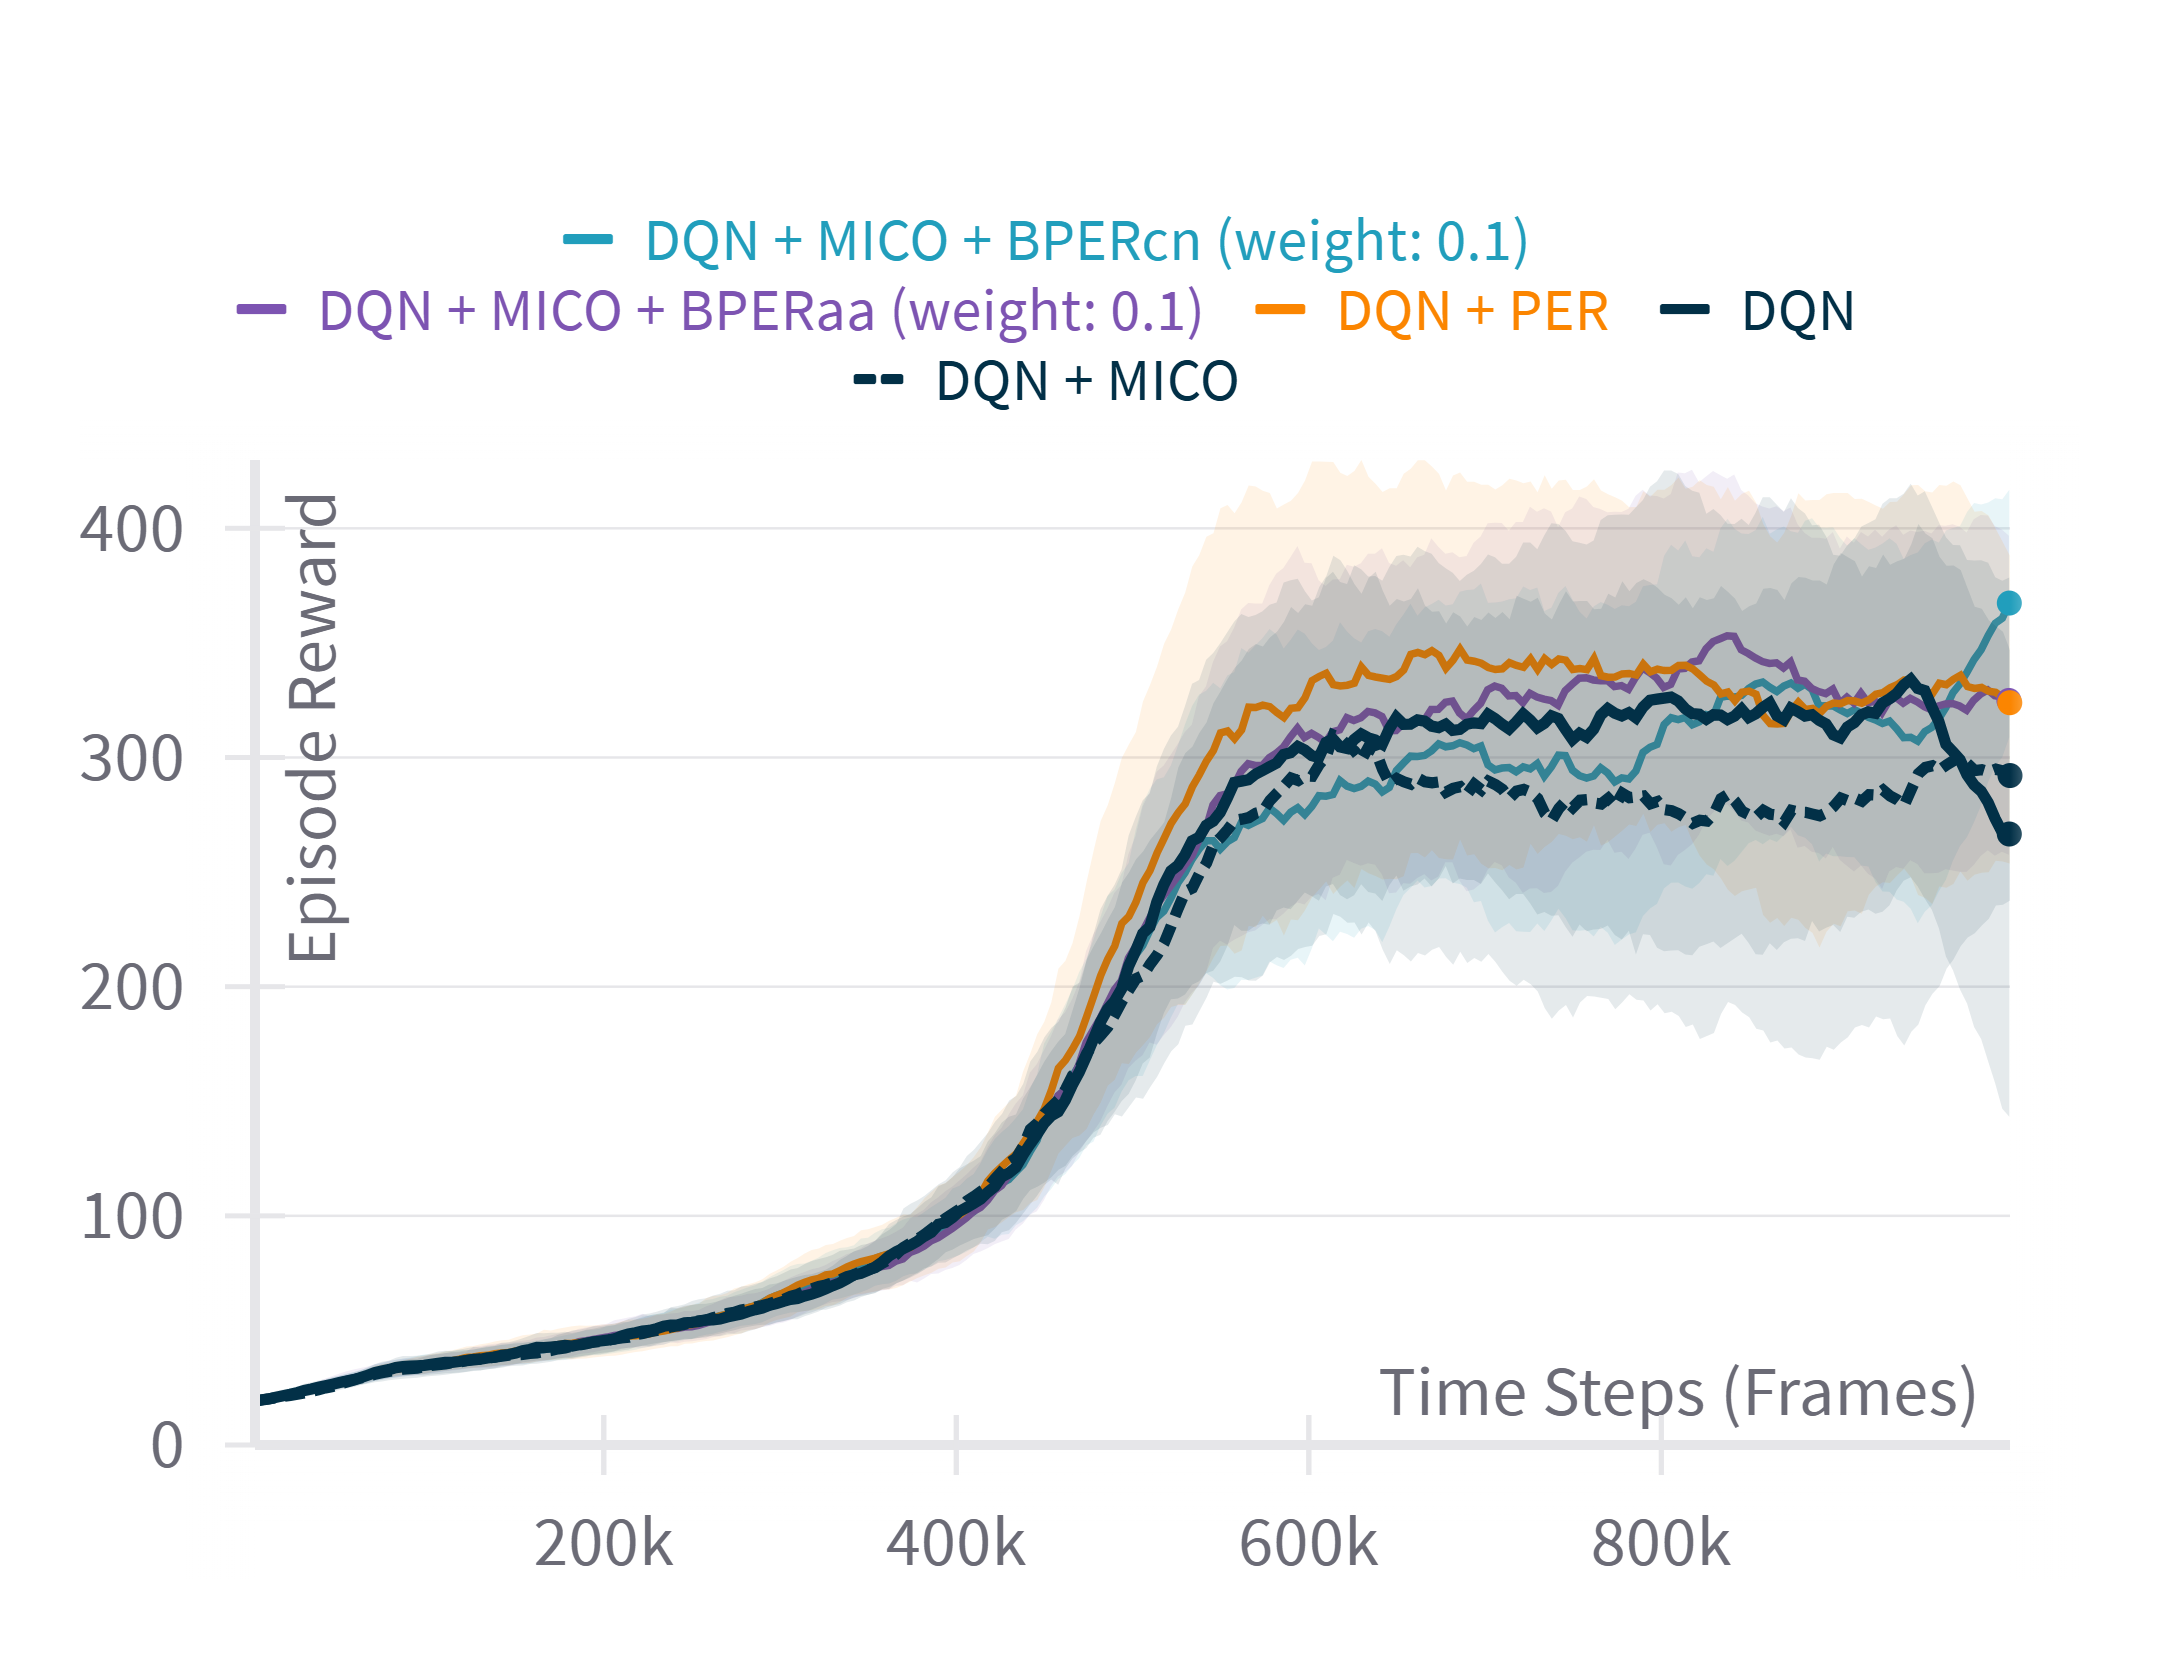
\includegraphics[width=\linewidth]{Results/general_results/episode_reward_cartpolev1.png}
        \caption{CartPole-v1}
        \label{fig:uniform_weighting}
    \end{subfigure}
    \hfill
    \begin{subfigure}{0.45\textwidth}
        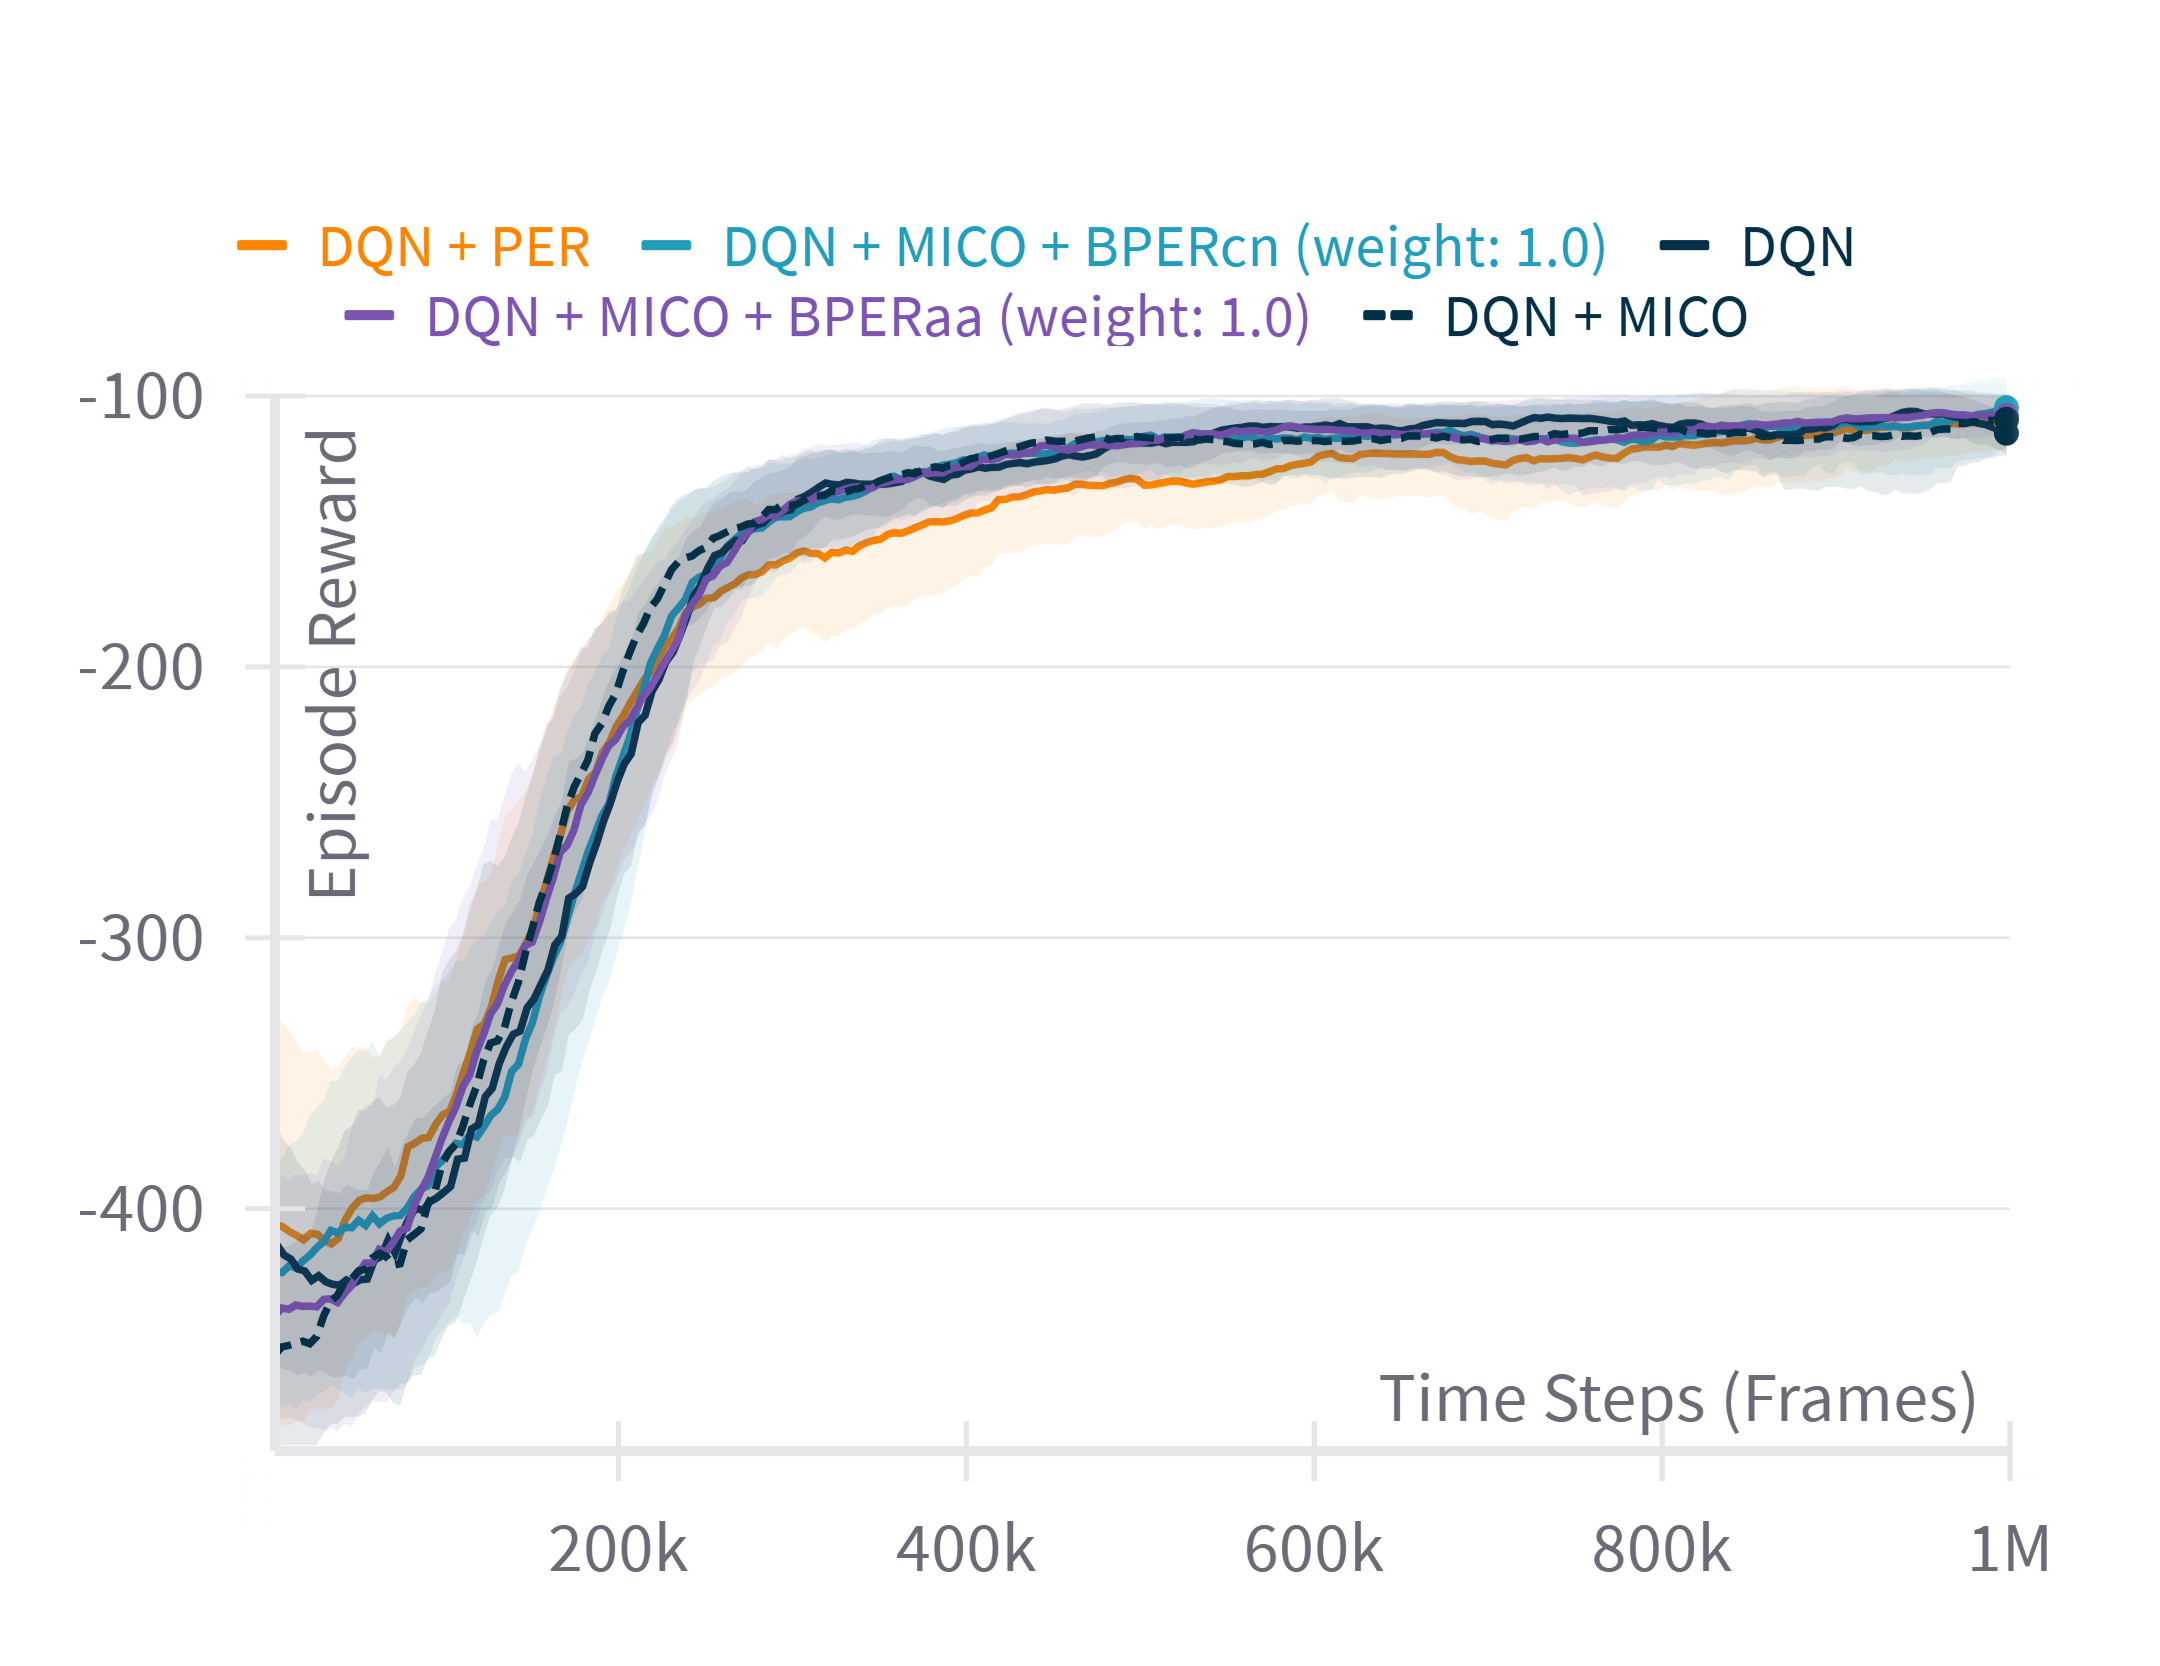
\includegraphics[width=\linewidth]{Results/general_results/episode_reward_acrobotv1.png}
        \caption{Acrobot-v1}
        \label{fig:uniform_weighting}
    \end{subfigure}
    \caption{Two images side-by-side}
    \label{fig:outdated_priorities}
\end{figure}

\begin{figure}[h]
    \centering
    \begin{subfigure}{0.45\textwidth}
    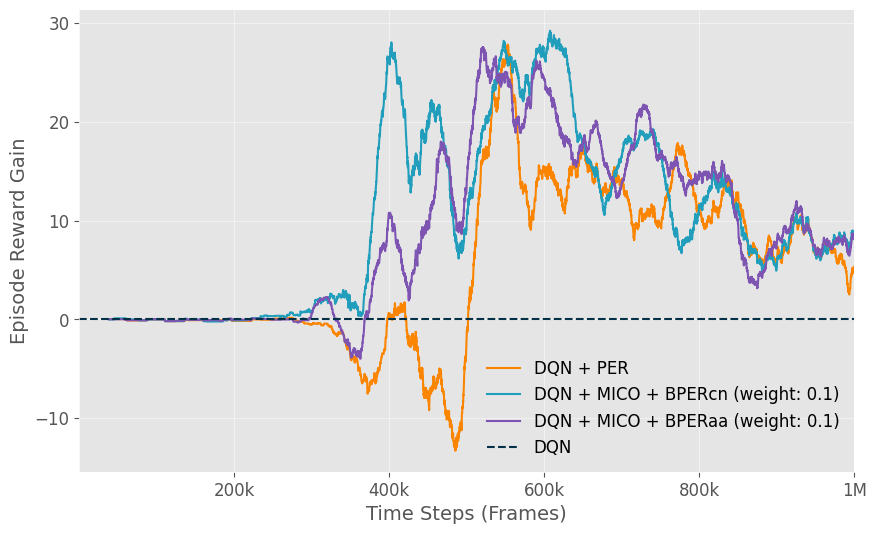
\includegraphics[width=\linewidth]{Results/general_results/mountain_car_reward_gain_vs_dqn.png}
        \caption{MountainCar-v0}
        \label{fig:on_policy_weighting}
    \end{subfigure}
    \hfill
    \begin{subfigure}{0.45\textwidth}
        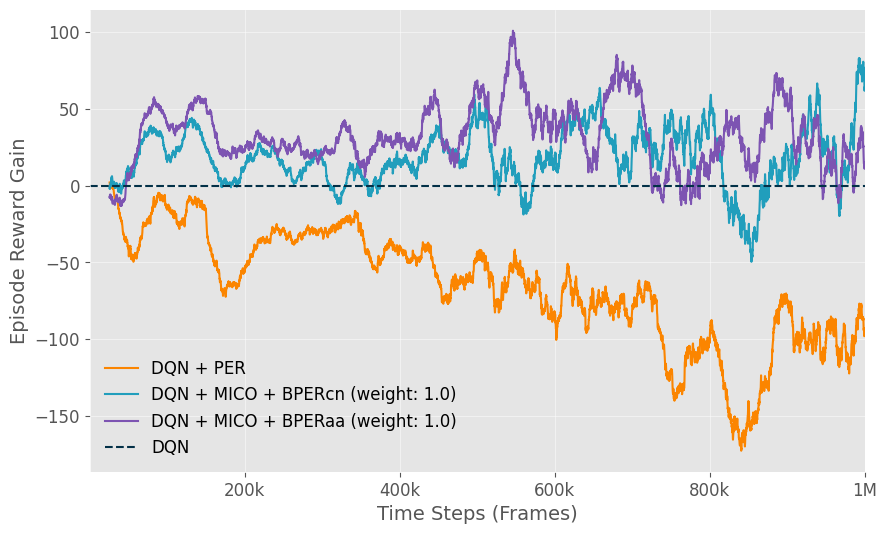
\includegraphics[width=\linewidth]{Results/general_results/lunarlander_reward_gain_vs_dqn.png}
        \caption{LunarLander-v1}
        \label{fig:uniform_weighting}
    \end{subfigure}
    \hfill
    \begin{subfigure}{0.45\textwidth}
        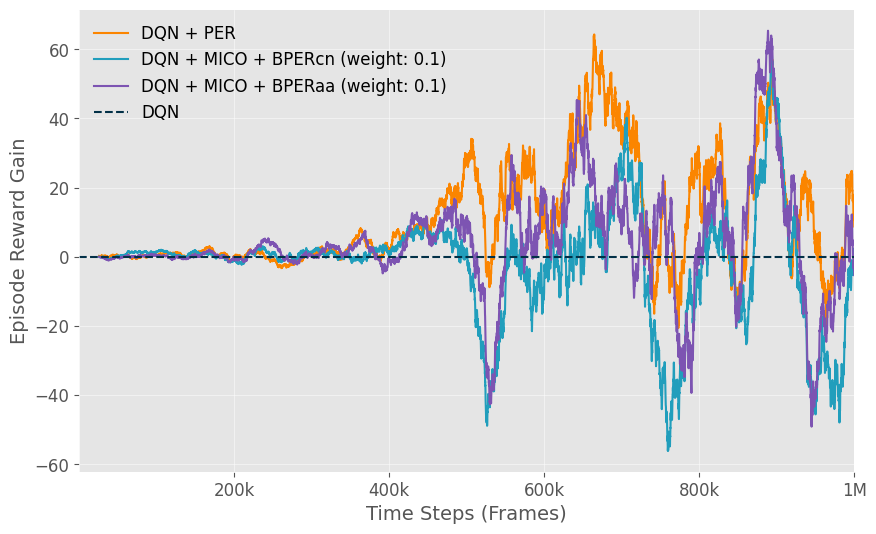
\includegraphics[width=\linewidth]{Results/general_results/cart_polev1_reward_gain_vs_dqn.png}
        \caption{CartPole-v1}
        \label{fig:uniform_weighting}
    \end{subfigure}
    \hfill
    \begin{subfigure}{0.45\textwidth}
        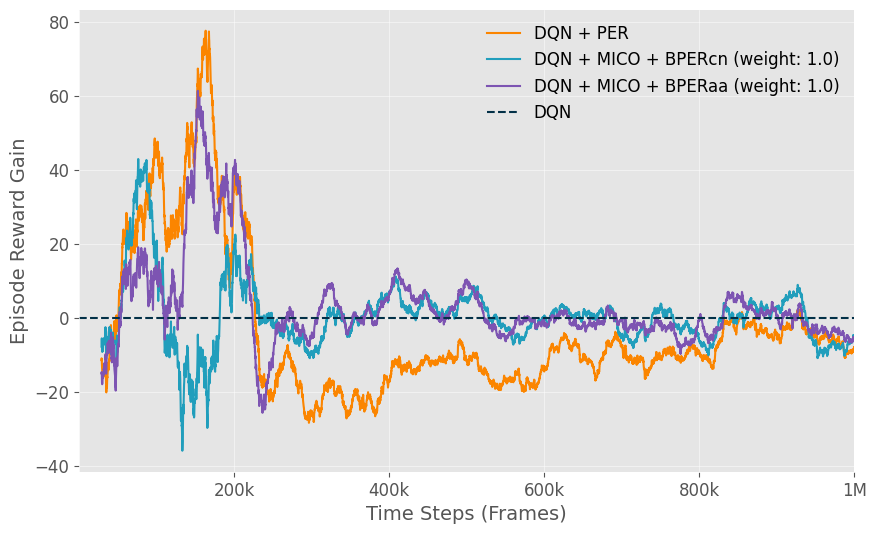
\includegraphics[width=\linewidth]{Results/general_results/acrobotv1_reward_gain_vs_dqn.png}
        \caption{Acrobot-v1}
        \label{fig:uniform_weighting}
    \end{subfigure}
    \caption{Two images side-by-side}
    \label{fig:outdated_priorities}
\end{figure}


% \begin{table}[h]
%     \centering
%     \caption{Performance Comparison of Different DQN Variants}
%     \label{tab:dqn_comparison}
%     \begin{tabular}{l >{\centering\arraybackslash}p{1.5cm} >{\centering\arraybackslash}p{1.5cm} >{\centering\arraybackslash}p{1.5cm} >{\centering\arraybackslash}p{1.5cm} >{\centering\arraybackslash}p{1.5cm} >{\centering\arraybackslash}p{1.5cm}}
%         \toprule
%                          & \multicolumn{2}{c}{\textbf{PER}}                       & \multicolumn{2}{c}{\textbf{BPERcn}}            & \multicolumn{2}{c}{\textbf{BPERaa}}             \\
%                          & {\color[HTML]{656565} \footnotesize DQN} & {\color[HTML]{656565} \footnotesize MICO} & {\color[HTML]{656565} \footnotesize DQN} & {\color[HTML]{656565} \footnotesize MICO} & {\color[HTML]{656565} \footnotesize DQN} & {\color[HTML]{656565} \footnotesize MICO} \\
%         \midrule
%         \textbf{MountainCar-v0} & $5.344 \pm 21.016$ & $39.088 \pm 39.151$   & $\mathbf{10.145} \pm \mathbf{21.471} $    & $\mathbf{43.889} \pm \mathbf{38.863}$  & $9.021 \pm 19.756$   & $42.765 \pm 39.060$     \\
%         \textbf{Cartpole-v1}    & $\mathbf{10.975} \pm \mathbf{133.140}$    & $\mathbf{24.23} \pm \mathbf{135.122}$   & $-2.100 \pm 134.322$   & $11.648 \pm 129.970$  & $3.790 \pm 134.959$    & $17.539 \pm 134.593$     \\
%         \textbf{Acrobot-v1}     & $-3.279 \pm 79.455$  & $-6.878 \pm 74.916$   & $0.250 \pm 78.057$    & $-3.350 \pm 73.122$  & $\mathbf{2.915} \pm \mathbf{75.618}$    & $\mathbf{-0.685} \pm \mathbf{70.853}$     \\
%         \textbf{LunarLander-v1} & $-65.620 \pm 175.613$    & $-107.075 \pm 183.781$   & $18.800 \pm 191.309$    & $-22.654 \pm 194.957$  & $\mathbf{32.125} \pm \mathbf{185.015}$    & $\mathbf{-9.330} \pm \mathbf{191.315}$   \\
%         \bottomrule
%     \end{tabular}
% \end{table}

\begin{table}[h]
    \hspace*{-1cm}
    \setlength{\tabcolsep}{2.5pt}
    \centering
    \begin{tabular}{llcccc}
        \toprule
        & \textbf{Baseline} & \textbf{MountainCar-v0} & \textbf{Cartpole-v1} & \textbf{Acrobot-v1} & \textbf{LunarLander-v1} \\
        \midrule
        {\footnotesize\textbf{PER}} & {\footnotesize\textbf{DQN}} & $5.344 \pm 21.016$ & $\mathbf{10.975} \pm \mathbf{133.140}$ & $-3.279 \pm 79.455$ & $-65.620 \pm 175.613$ \\
         & {\footnotesize\textbf{MICO}} & $39.088 \pm 39.151$ & $\mathbf{24.23} \pm \mathbf{135.122}$ & $-6.878 \pm 74.916$ & $-107.075 \pm 183.781$ \\
        {\footnotesize\textbf{BPERcn}} & {\footnotesize\textbf{DQN}} & $\mathbf{10.145} \pm \mathbf{21.471}$ & $-2.100 \pm 134.322$ & $0.250 \pm 78.057$ & $18.800 \pm 191.309$ \\
        & {\footnotesize\textbf{MICO}} & $\mathbf{43.889} \pm \mathbf{38.863}$ & $11.648 \pm 129.970$ & $-3.350 \pm 73.122$ & $-22.654 \pm 194.957$ \\
        {\footnotesize\textbf{BPERaa}} & {\footnotesize\textbf{DQN}} & $9.021 \pm 19.756$ & $3.790 \pm 134.959$ & $\mathbf{2.915} \pm \mathbf{75.618}$ & $\mathbf{32.125} \pm \mathbf{185.015}$ \\
        & {\footnotesize\textbf{MICO}} & $42.765 \pm 39.060$ & $17.539 \pm 134.593$ & $\mathbf{-0.685} \pm \mathbf{70.853}$ & $\mathbf{-9.330} \pm \mathbf{191.315}$ \\
        \bottomrule
    \end{tabular}
    \caption{Performance Comparison of Different DQN Variants}
    \label{tab:dqn_comparison_transposed}
\end{table}

\begin{figure}[h]
    \centering
    \begin{subfigure}{0.45\textwidth}
    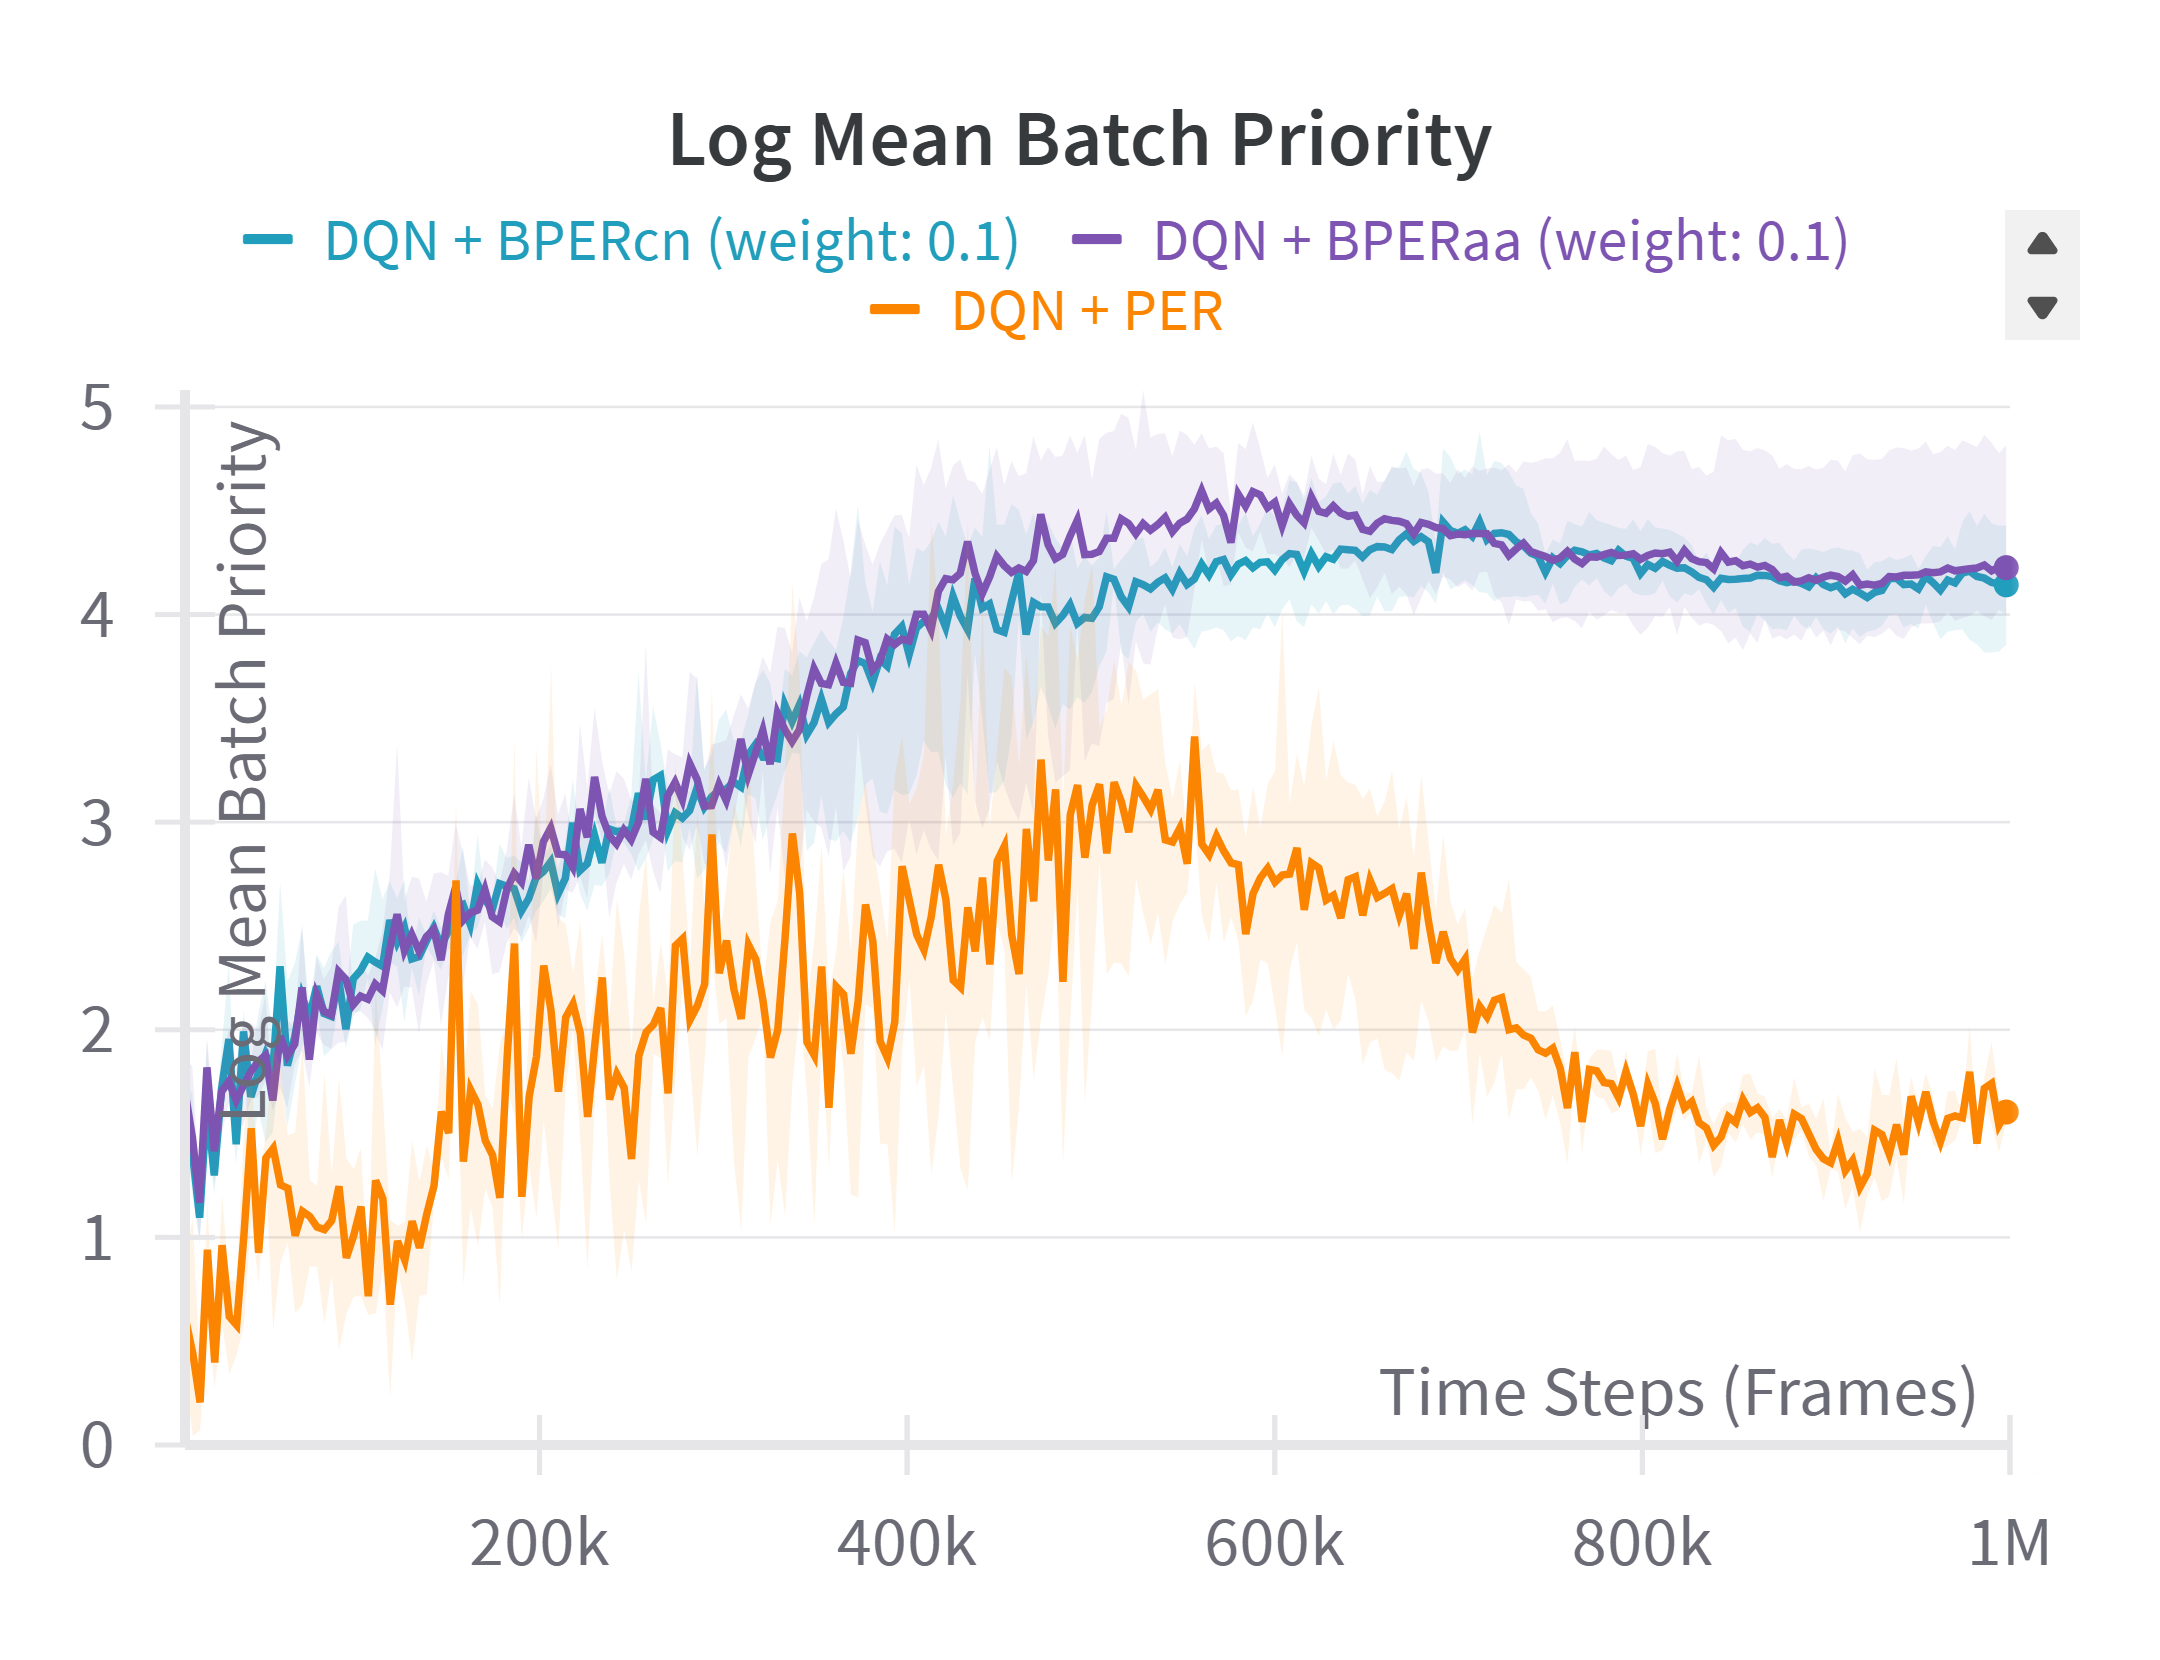
\includegraphics[width=\linewidth]{Results/general_results/log_mean_batch_priority_mountain_car.png}
        \caption{MountainCar-v0}
        \label{fig:on_policy_weighting}
    \end{subfigure}
    \hfill
    \begin{subfigure}{0.45\textwidth}
        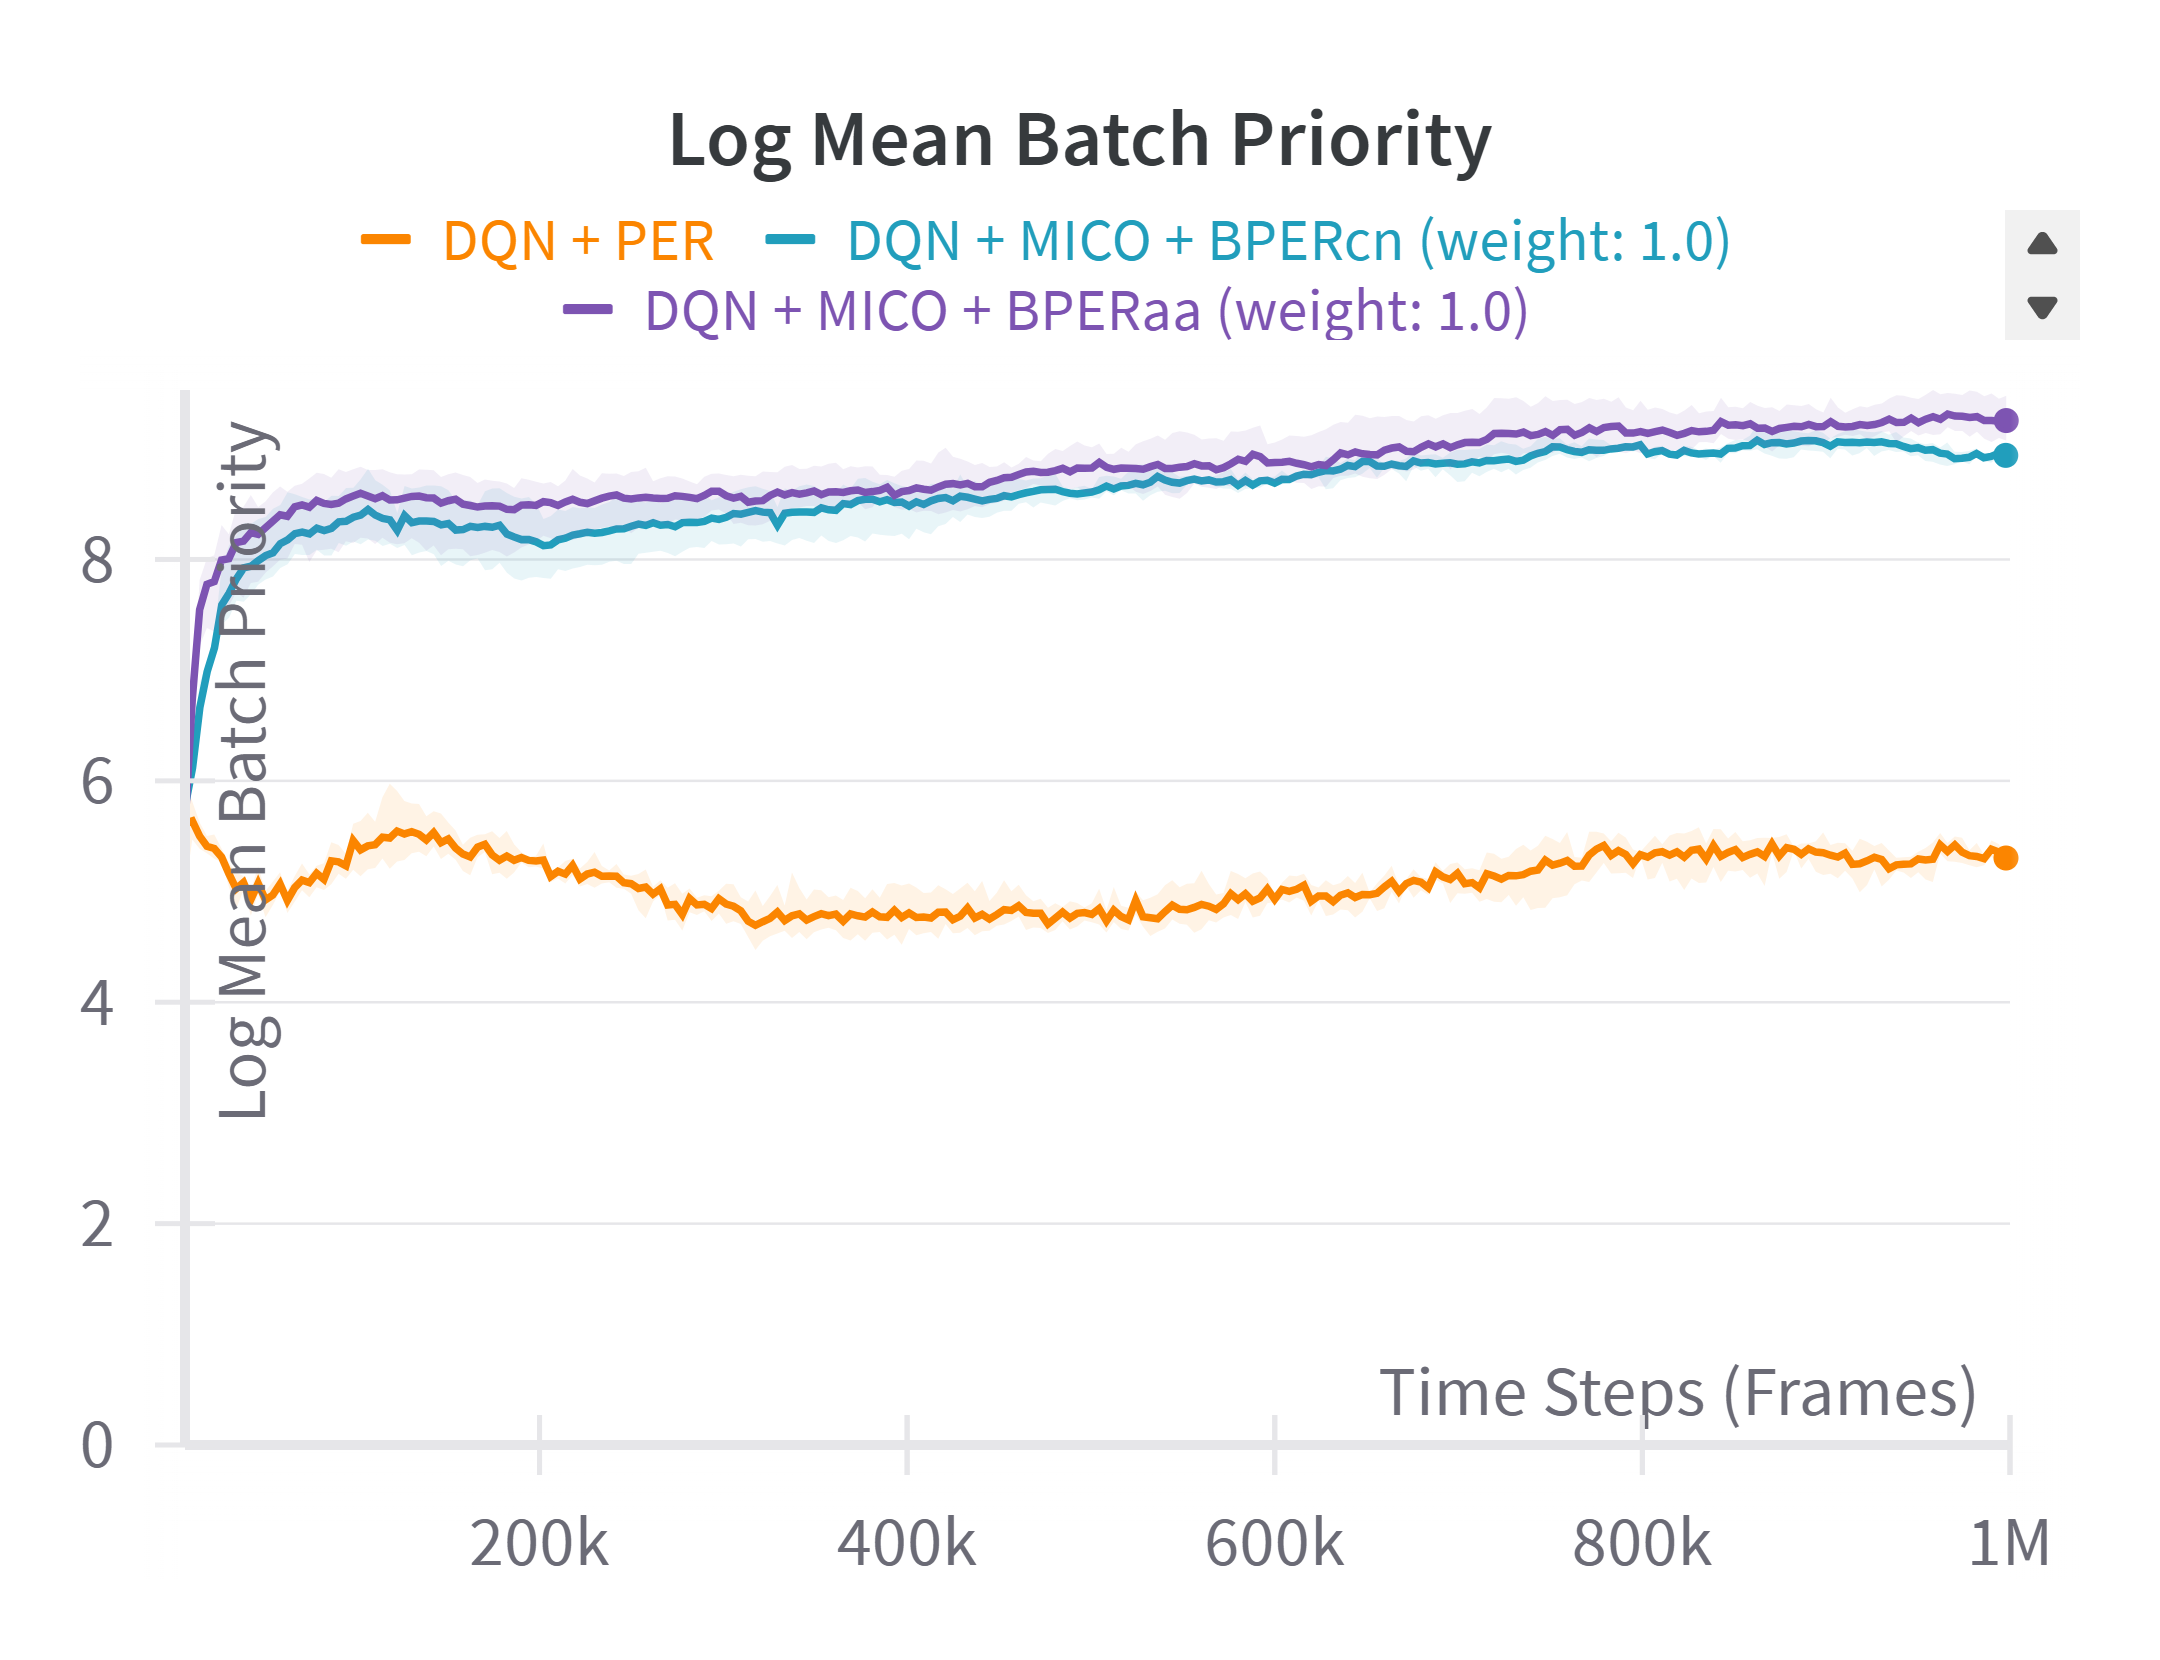
\includegraphics[width=\linewidth]{Results/general_results/log_mean_batch_priority_lunarlander.png}
        \caption{LunarLander-v1}
        \label{fig:uniform_weighting}
    \end{subfigure}
    \hfill
    \begin{subfigure}{0.45\textwidth}
        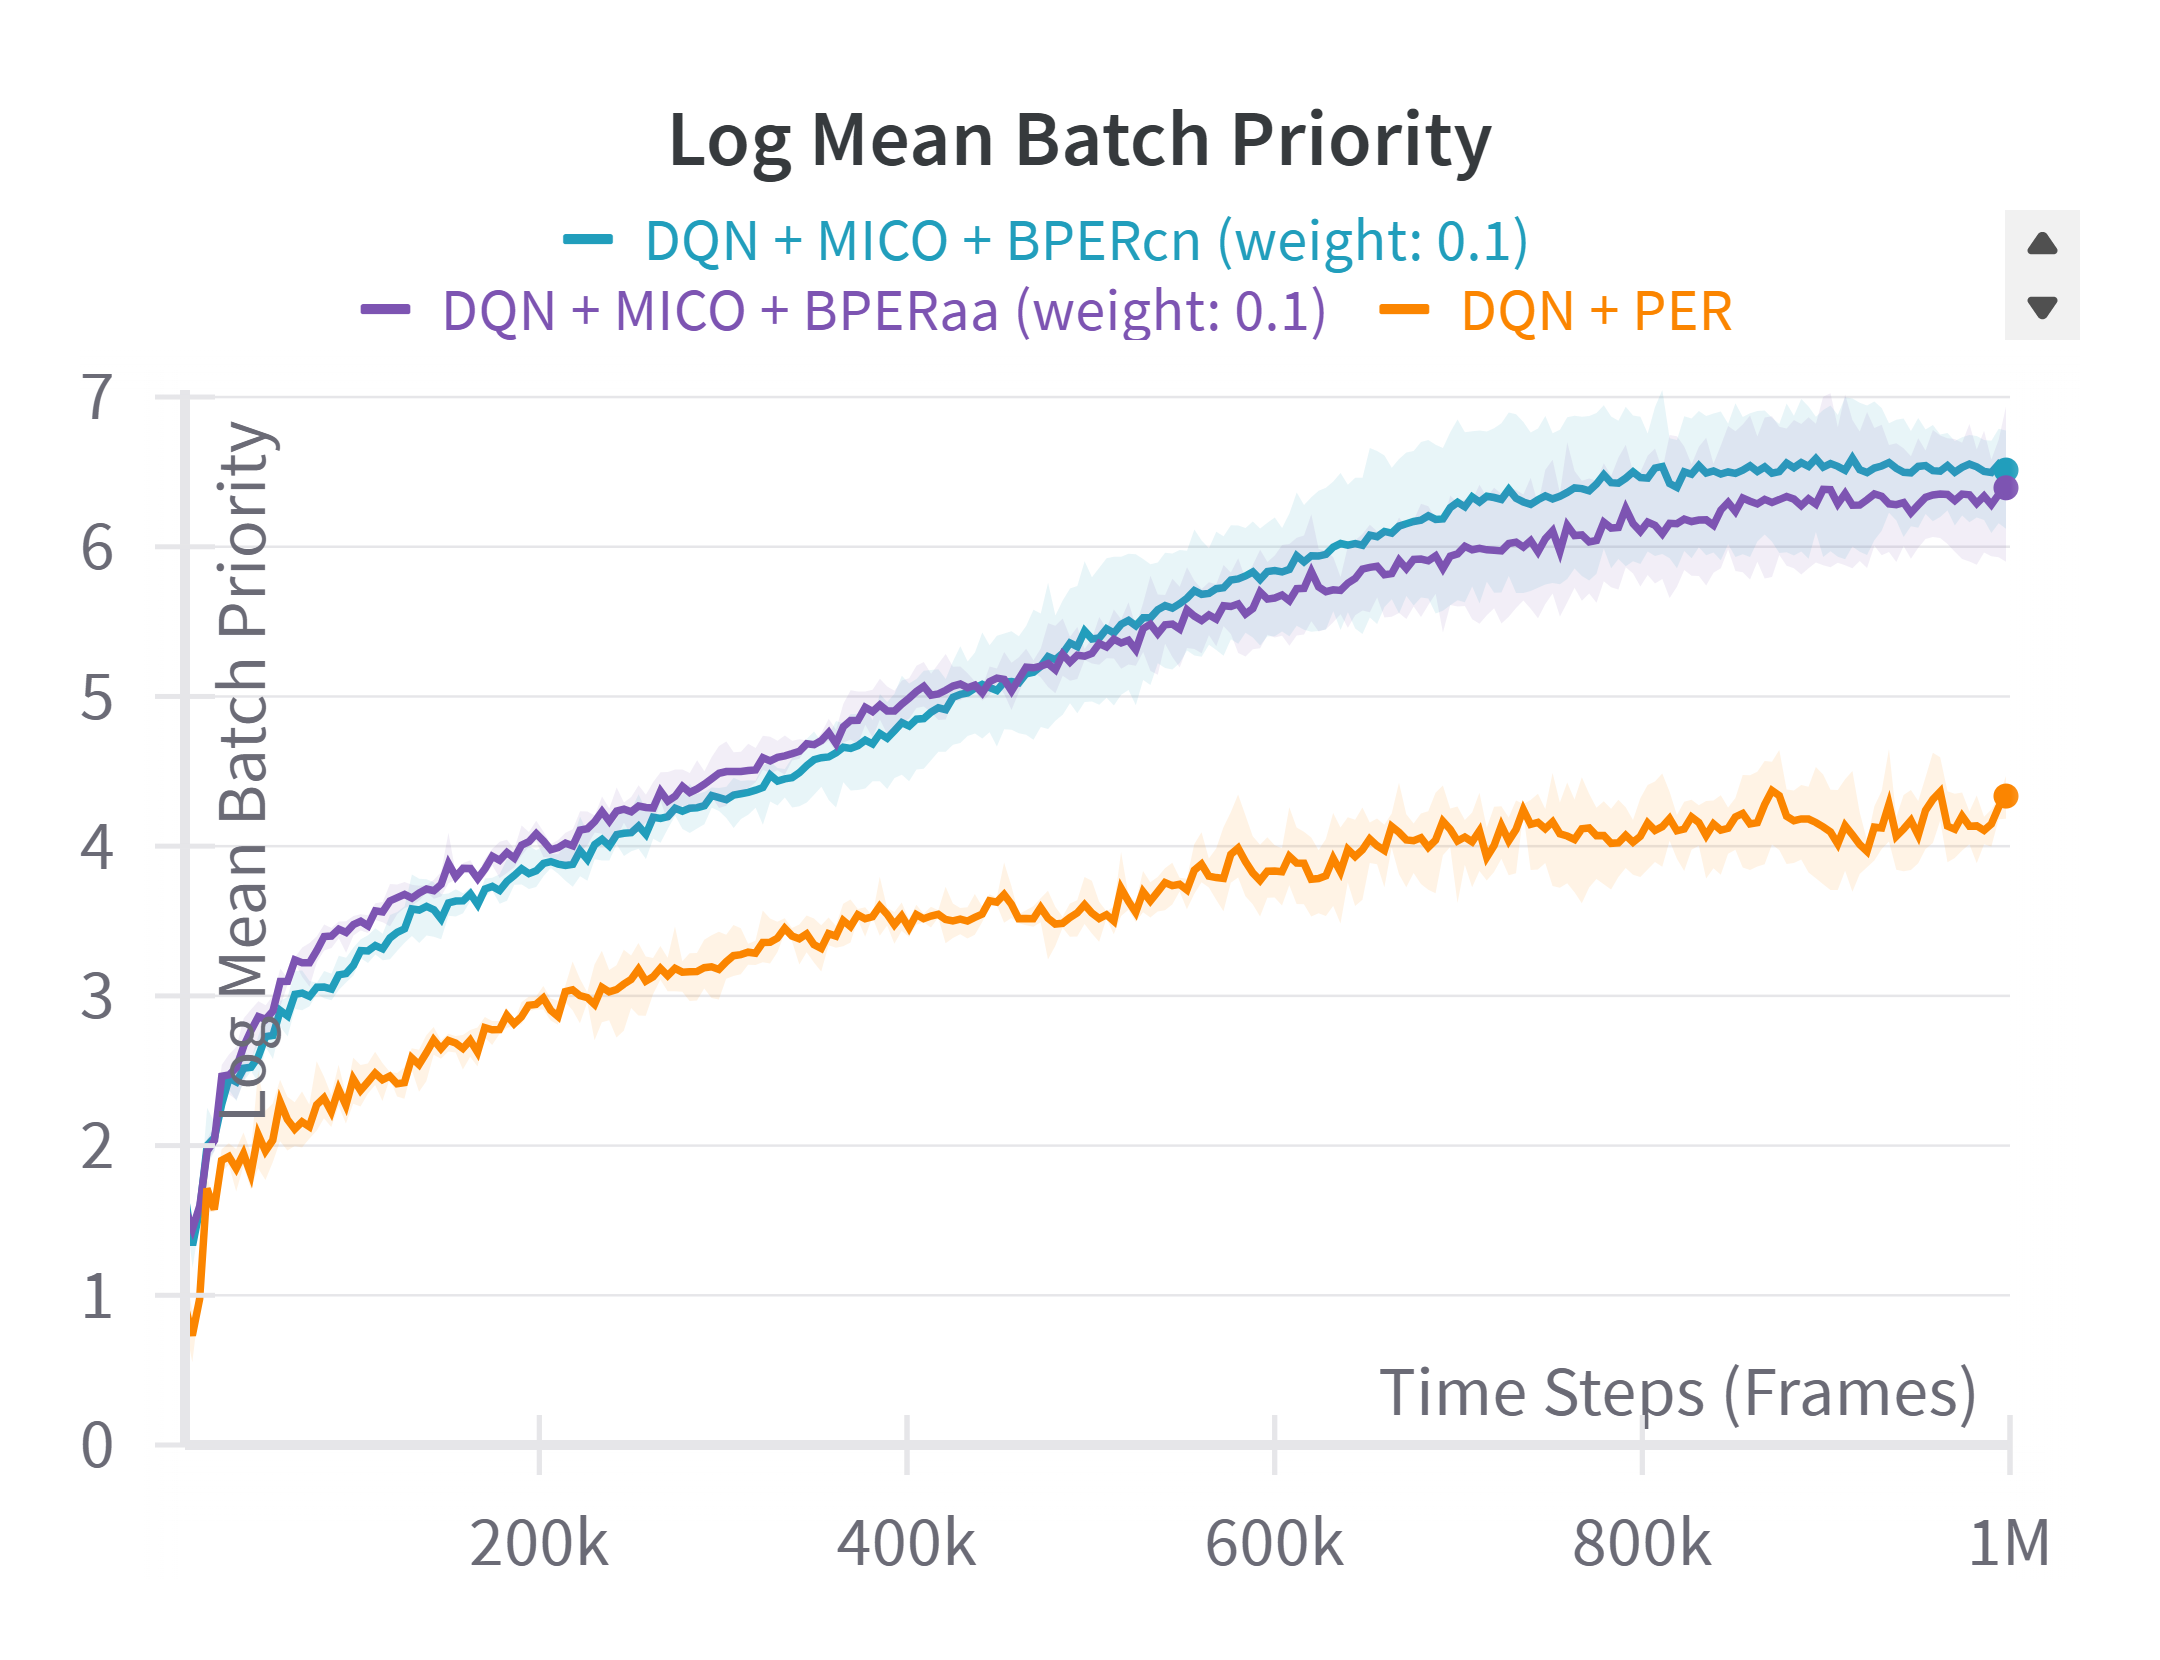
\includegraphics[width=\linewidth]{Results/general_results/log_mean_batch_priority_cartpolev1.png}
        \caption{CartPole-v1}
        \label{fig:uniform_weighting}
    \end{subfigure}
    \hfill
    \begin{subfigure}{0.45\textwidth}
        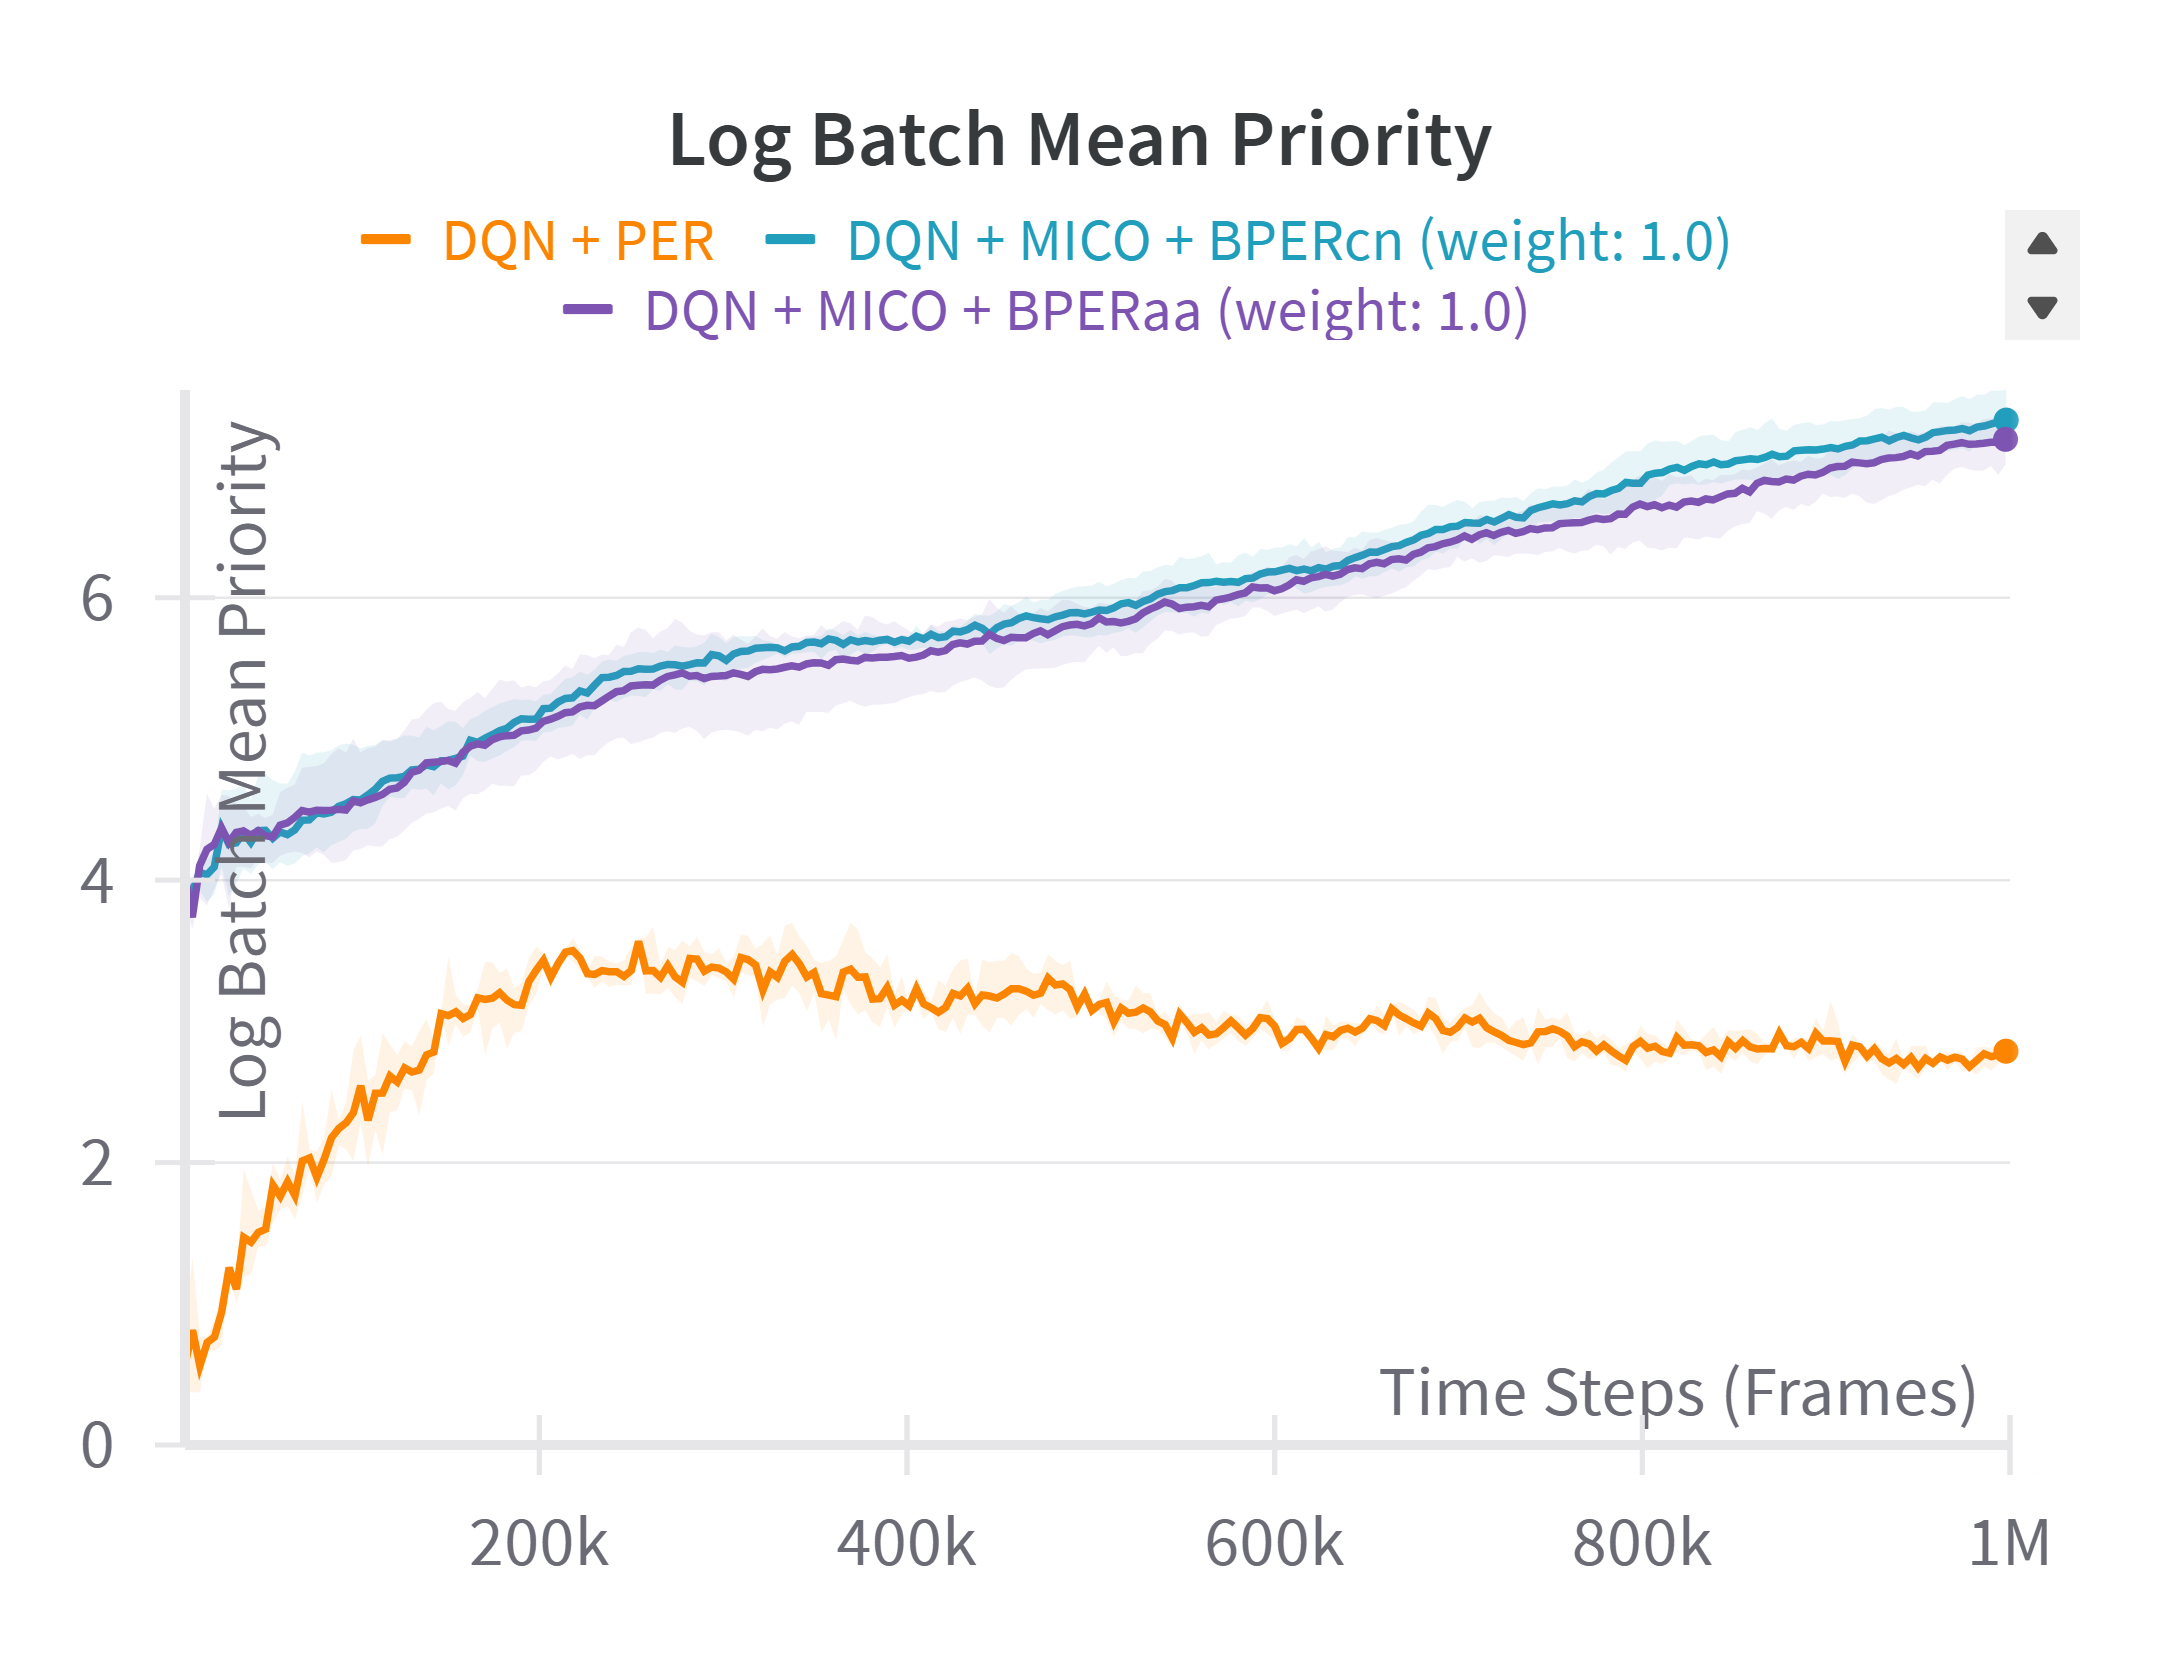
\includegraphics[width=\linewidth]{Results/general_results/log_mean_batch_priority_acrobot.png}
        \caption{Acrobot-v1}
        \label{fig:uniform_weighting}
    \end{subfigure}
    \caption{Two images side-by-side}
    \label{fig:outdated_priorities}
\end{figure}

% % !TEX root =  ../Dissertation.tex

\chapter{Conclusion and Future Work}

Even though it returns promising results, one thing that I realized is that the bisimulation values are relative too high compare with the td-errors, which can produce to focus too much in some experiences and unven and drastically skewness probability distribution, a way to soft the sampling distribution could be recommended. 

We have tried to normalize using a logaritmic scale and max min, but it didn't worked properly.

Even when using the 0.01 beta in the loss function

Theoretical proof

It lacks of a theoretical basis

also some experimetns suggest that most of the improvements comes from the MICO and not actually the prioritization

a sweep over the alpha and beta values, although we use the best one for PER, they could not be the best ones for BPER

Additionally, a way to normalize the priorities or another sampling method like the rank based because the BPER priorities are larger than the td-error (ojo).

Try Double DQN and other algorithms and better benchmarks.

Check with more state of the art algorithms and methods


We hypothesis that earlier improvement on BPERcn and BPERaa are more related with randomly picking different distant states in the beginning. However, over time as the metric is learn, the BPERaa because a better indicator of bisimilar transtion (or more informative transition), particularly for the scarce and highly variable approximatation mention in [], and the motive for what Strategy 2 was actually proposed.

% VISA

% For visits of up to 6 months for most purposes.
% Cost: CAN \$100

% https://neurips.cc/Conferences/2024/Dates

% https://www.canada.ca/en/immigration-refugees-citizenship/services/visit-canada/about-visitor-visa.html

% https://www.canada.ca/content/dam/ircc/documents/pdf/english/kits/forms/imm5645/01-01-2021/imm5645e.pdf

% https://www.canada.ca/en/immigration-refugees-citizenship/services/visit-canada/apply-visitor-visa.html
% % !TEX root =  ../Dissertation.tex

\chapter{Chapter Title}


% % !TEX root =  ../Dissertation.tex

\chapter{Chapter Title}


% % !TEX root =  ../Dissertation.tex

\chapter{Chapter Title}


% % !TEX root =  ../Dissertation.tex

\chapter{Chapter Title}



\bibliographystyle{abbrv}
\bibliography{bibliography}

\appendix
\chapter{Appendices}
% \addcontentsline{toc}{chapter}{Appendices}

\section{Metrics}
\label{append:metrics}

The following information was retrieved from the Supplementary Material provide by Castro et al. \cite{castro2021mico}. 

A \textbf{metric} \(d\) on a set \(X\) is a function \(d : X \times X \to [0, \infty)\) respecting the following axioms for any \(x, y, z \in X\):

\begin{enumerate}
    \item \textbf{Identity of indiscernibles:} \(d(x, y) = 0 \iff x = y\);
    \item \textbf{Symmetry:} \(d(x, y) = d(y, x)\);
    \item \textbf{Triangle inequality:} \(d(x, y) \leq d(x, z) + d(z, y)\).
\end{enumerate}

A \textbf{pseudometric} is similar, but the "identity of indiscernibles" axiom is weakened:

\begin{enumerate}
    \item \(x = y \implies d(x, y) = 0\);
    \item \(d(x, y) = d(y, x)\);
    \item \(d(x, y) \leq d(x, z) + d(z, y)\).
\end{enumerate}

Note that the weakened first condition \emph{does} allow one to have \(d(x, y) = 0\) when \(x \neq y\).

A \textbf{(pseudo)metric space} \((X, d)\) is defined as a set \(X\) together with a (pseudo)metric \(d\) defined on \(X\).

A \textbf{diffuse metric} is similar to as pseudometri, but the 'identity of indiscernibles' axiom is weakened even more:

\begin{enumerate}
    \item \(d(x, y) \geq 0\) for any $x, y \in X$;
    \item \(d(x, y) = d(y, x)\);
    \item \(d(x, y) \leq d(x, z) + d(z, y)\).
\end{enumerate}

Note that the weakened first condition \emph{does} allow one to have self-distance greater than zero $d(x,x) > 0$.

\section{Algorithm: DQN with Matching under Independent Couplings (MICo)}
\label{append:dqn_mico}

\begin{algorithm}[H]
\caption{DQN with Matching under Independent Couplings (MICo)}
\label{algorithm:dqn_mico}
\begin{algorithmic}[1]
\State \textbf{Input:} minibatch $k$, step-size $\eta$, replay period $K$ and size $N$, budget $T$ (total steps).
\State \textbf{Initialize} action-value function $Q$ with random weights $\xi$, $\omega$
\State \textbf{Initialize} target action-value function $Q^-$ with weights $\{\bar{\xi},\bar{\omega}\} \leftarrow \{\xi, \omega\}$
\State \textbf{Initialize} replay memory $\mathcal{D} = \emptyset$ with capacity $N$%$\Delta_{\{\xi, \omega\}} = 0$, $\Delta_\omega = 0$, $p_1 = 1$
% \State Observe $s_0$ and choose $a_0 \sim \pi^\epsilon_\theta(s_0)$ 
\For{$t = 1$ to $T$}
    \State Observe $s_t$
    \State Choose action $a_t \sim \pi^\epsilon_\theta(s_t)$
    \State Execute action $a_t$ and observe $r_t$ and $s_{t+1}$
    \State Store transition $(s_t, a_t, r_t, s_{t+1})$ in $\mathcal{D}$
    \If{$t \equiv 0 \mod K$}
        % \For{$j = 1$ to $k$}
        \State Sample minibatch $B \sim \text{Uniform}(\mathcal{D})$ of transitions $e_j$        % \State Compute importance-sampling weight $w_j = \left( N \cdot P(j) \right)^{-\beta} / \max_i w_i$
        \State Set $y_j = 
        \begin{cases} 
            r_j & \text{for terminal } s_{j+1}\\
            r_j + \gamma \max_{a'} Q^-(s_{j+1}, a'; \{\bar{\xi},\bar{\omega}\}) & \text{otherwise}
        \end{cases}$
        \State Compute TD-error $\delta_j = y_j - Q(s_{j}, a_{j}; \{\xi, \omega\})$, and loss $\mathcal{L}_{\text{TD}} = \delta_j^2 $
        \State Squarify minibatch $B$ to get transition pairs $\left\langle x, r_x, x^{\prime}\right\rangle,\left\langle y, r_y, y^{\prime}\right\rangle$ 
        \State Compute MICo loss $\mathcal{L}_{\text{MICo}} = \left(T_{\bar{\omega}}^U\left(r_x, x^{\prime}, r_y, y^{\prime}\right)-U_\omega(x, y)\right)^2$
        \State Compute total loss $\mathcal{L}_\alpha(\xi, \omega) = (1 - \alpha) \mathcal{L}_{\text{TD}}(\xi, \omega) + \alpha \mathcal{L}_{\text{MICo}}(\omega)$
        \State Perform a gradient descent step on $\mathcal{L}_\alpha(\xi, \omega)$
        % \State Update transition priority $p_j \leftarrow (1 - \mu) |\delta_j| + \mu U_\omega(s_j,s_{j+1}) + \epsilon$
        \State Every C optimizing steps update $\{\bar{\xi},\bar{\omega}\} \leftarrow \{\xi, \omega\}$
        

        
        % \State Accumulate weight-change $\Delta_{\{\xi, \omega\}} \leftarrow \Delta_{\{\xi, \omega\}} + w_j \cdot \delta_j \cdot \nabla_\theta Q(s_{j}, a_{j})$
        % \State Compute bisimulation distance error $\sigma_j = T_{\bar{\omega}}^U\left(r_x, x^{\prime}, r_y, y^{\prime}\right)-U_\omega(x, y)$
        %  \State Accumulate weight-change $\Delta_{\omega} \leftarrow \Delta_{\omega} + w_j \cdot \sigma_j \cdot \nabla_\omega U_\omega(s_{i}, a_{j})$   

        % \EndFor
        % \State Update weights $\theta \leftarrow \theta + \eta \cdot \Delta$, reset $\Delta = 0$
    \EndIf
\EndFor
\end{algorithmic}
\end{algorithm}

\section{Distance between Priority Sampling Distributions}

% Given the sampling distribution of priorities pi(·) from the experience buffer and
% the corresponding ideal distribution p
% ∗
% i
% (·) (theoretically achieved when all state
% space priorities are updated at each time step7
% ), 1) the on-policy weighting is
% given by P31
% j=1 w
% π
% (sj )|pi(sj ) − p
% ∗
% i
% (sj )|, i ∈ {1, 2}, and 2) the uniform weighting is
% 1
% 31
% P31
% j=1 |pi(sj ) − p
% ∗
% i
% (sj )|, i ∈ {1, 2}, where p1 corresponds to the PER method and
% p2 corresponds to the BPER method. A more detailed explanation of this procedure
% is provided in the Appendix ??.

\section{Hyperparameters Setting}
\label{append:hyperparameters}

\begin{table}[H]
\centering

\hspace*{-1cm}
\begin{tabular}{@{} lccccc @{}}
\toprule
& \textbf{Hyperparameter} & {\footnotesize\textbf{DQN}} & {\footnotesize \textbf{DQN PER}} & {\footnotesize\textbf{DQN MICo}} & {\footnotesize\textbf{DQN BPER}} \\ 
\midrule

\multirow{8}{*}{\textbf{Collector}} 
& Total Budget & 100,000 & 100,000 & 100,000 & 100,000 \\ 
& Replay Period & 128 & 128 & 128 & 128 \\ 
& Eps Start & 0.1 & 0.1 & 0.1 & 0.1 \\ 
& Eps End & 0.005 & 0.005 & 0.005 & 0.005 \\ 
& Eps Annealing Frames & 520,000 & 520,000 & 520,000 & 520,000 \\ 
& Init Random Frames & 200 & 200 & 200 & 200 \\ 
& Frame Stack & 1 & 1 & 1 & 1 \\
& Frame Skip & 1 & 1 & 1 & 1 \\ 
\midrule

\multirow{5}{*}{\textbf{Policy}} 
& CNN Net (Cells) & [32, 64, 64] & [32, 64, 64] & [32, 64, 64] & [32, 64, 64] \\ 
& Kernel Sizes & [8, 4, 3] & [8, 4, 3] & [8, 4, 3] & [8, 4, 3] \\ 
& Strides & [4, 2, 1] & [4, 2, 1] & [4, 2, 1] & [4, 2, 1] \\ 
& MLP Net (Cells) & [64, 64] & [64, 64] & [64, 64] & [64, 64] \\ 
& Activation & ReLU & ReLU & ReLU & ReLU \\ 
\midrule

\multirow{5}{*}{\textbf{Buffer}} 
& Buffer Size & 100,000 & 100,000 & 100,000 & 100,000 \\ 
& Batch Size & 256 & 256 & 256 & 256 \\ 
& Alpha & -- & 0.6 & -- & 0.6 \\ 
& Beta & -- & 0.4 & -- & 0.4 \\ 
& Priority Weight & -- & -- & 1.0 & 1.0 \\ 
\midrule

\multirow{4}{*}{\textbf{Optim}} 
& Learning Rate & 0.0015 & 0.0015 & 0.0015 & 0.0015 \\ 
& Max Grad Norm & 10 & 10 & 10 & 10 \\ 
& Weight Decay & 0.00001 & 0.00001 & 0.00001 & 0.00001 \\ 
& Eps & 1.5e-4 & 1.5e-4 & 1.5e-4 & 1.5e-4 \\ 
\midrule

\multirow{6}{*}{\textbf{Loss}} 
& Gamma & 0.99 & 0.99 & 0.99 & 0.99 \\ 
& MICO Weight & -- & -- & 0.01 & 0.01 \\ 
& MICO Beta & -- & -- & 0.1 & 0.1 \\ 
& MICO Gamma & -- & -- & 0.99 & 0.99 \\ 
& Hard Update Freq & 50 & 50 & 50 & 50 \\ 
& Num Updates & 1 & 1 & 1 & 1 \\ 
\bottomrule

\end{tabular}
\caption[Hyperparameter Configurations for Grid World]{\textbf{Hyperparameter Configurations for Grid World.} This configuration was consistently used among different independent runs, where the setting for DQN BPER works for both BPERcn and BPERaa.}
\end{table}

\begin{table}[H]
\centering

\hspace*{-1cm}
\begin{tabular}{@{} lccccc @{}}
\toprule
& \textbf{Hyperparameter} & {\footnotesize\textbf{DQN}} & {\footnotesize \textbf{DQN PER}} & {\footnotesize\textbf{DQN MICo}} & {\footnotesize\textbf{DQN BPER}} \\ 
\midrule

\multirow{8}{*}{\textbf{Collector}} 
& Total Budget & 1,000,064 & 1,000,064 & 1,000,064 & 1,000,064 \\ 
& Replay Period & 128 & 128 & 128 & 128 \\ 
& Eps Start & 0.5 & 0.5 & 0.5 & 0.5 \\ 
& Eps End & 0.005 & 0.005 & 0.005 & 0.005 \\ 
& Eps Annealing Frames & 520,000 & 520,000 & 520,000 & 520,000 \\ 
& Init Random Frames & 20,000 & 20,000 & 20,000 & 20,000 \\ 
& Frame Stack & 4 & 4 & 4 & 4 \\
& Frame Skip & 4 & 4 & 4 & 4 \\ 
\midrule

\multirow{5}{*}{\textbf{Policy}} 
& CNN Net (Cells) & [32, 64, 64] & [32, 64, 64] & [32, 64, 64] & [32, 64, 64] \\ 
& Kernel Sizes & [8, 4, 3] & [8, 4, 3] & [8, 4, 3] & [8, 4, 3] \\ 
& Strides & [4, 2, 1] & [4, 2, 1] & [4, 2, 1] & [4, 2, 1] \\ 
& MLP Net (Cells) & [64, 64] & [64, 64] & [64, 64] & [64, 64] \\ 
& Activation & ReLU & ReLU & ReLU & ReLU \\ 
\midrule

\multirow{5}{*}{\textbf{Buffer}} 
& Buffer Size & 100,000 & 100,000 & 100,000 & 100,000 \\ 
& Batch Size & 256 & 256 & 256 & 256 \\ 
& Alpha & -- & 0.6 & -- & 0.6 \\ 
& Beta & -- & 0.4 & -- & 0.4 \\ 
& Priority Weight & -- & -- & 1.0 & 1.0 \\ 
\midrule

\multirow{4}{*}{\textbf{Optim}} 
& Learning Rate & 0.0015 & 0.0015 & 0.0015 & 0.0015 \\ 
& Max Grad Norm & 10 & 10 & 10 & 10 \\ 
& Weight Decay & 0.00001 & 0.00001 & 0.00001 & 0.00001 \\ 
& Eps & 1.5e-4 & 1.5e-4 & 1.5e-4 & 1.5e-4 \\ 
\midrule

\multirow{6}{*}{\textbf{Loss}} 
& Gamma & 0.99 & 0.99 & 0.99 & 0.99 \\ 
& MICO Weight & -- & -- & 0.01 & 0.01 \\ 
& MICO Beta & -- & -- & 0.1 & 0.1 \\ 
& MICO Gamma & -- & -- & 0.99 & 0.99 \\ 
& Hard Update Freq & 50 & 50 & 50 & 50 \\ 
& Num Updates & 1 & 1 & 1 & 1 \\ 
\bottomrule

\end{tabular}
\caption[Hyperparameter Configurations for Other Environments]{\textbf{Hyperparameter Configurations for Other Environments.} This configuration was consistently applied across the MountainCar, CartPole, Acrobot, and LunarLander environments for each independent run. The settings for DQN BPER are applicable to both BPERcn and BPERaa. The priority weight configuration was adjusted as described in the results.}
\end{table}


\section{Priority Weight Sweep Results}
\label{append:priority_weight_sweep}

\begin{figure}[H]
    \centering
    \begin{subfigure}{0.45\textwidth}
    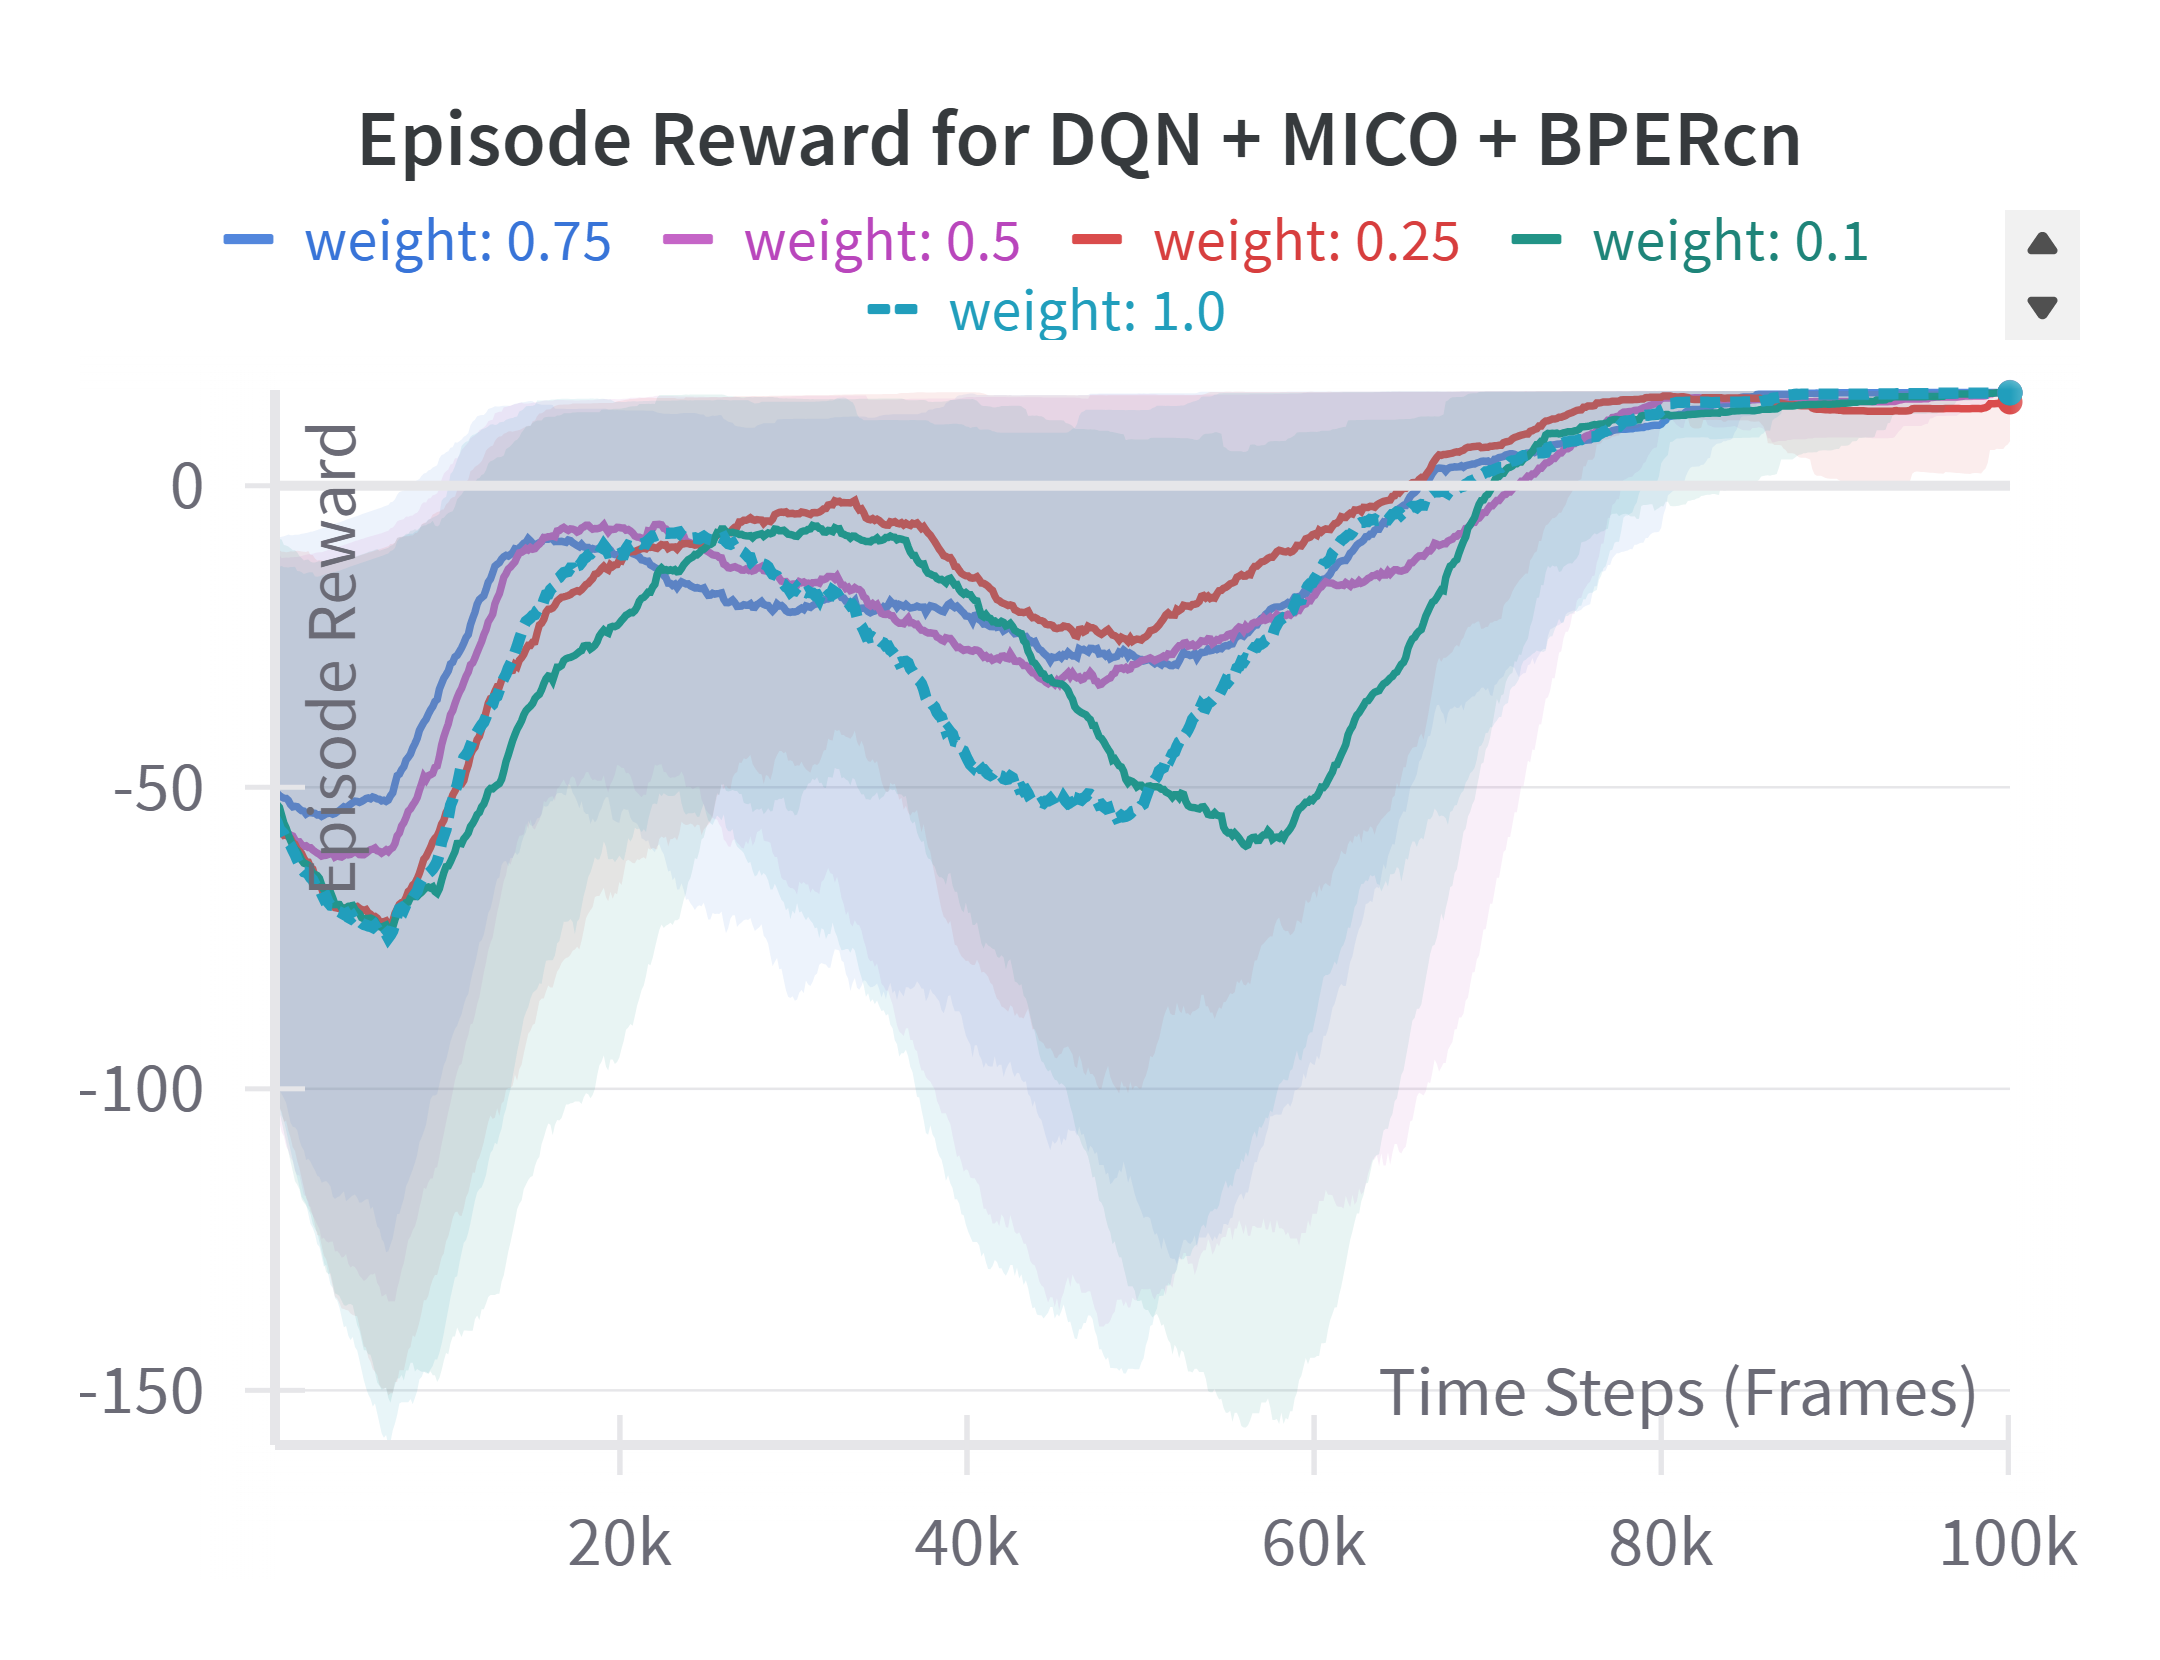
\includegraphics[width=\linewidth]{Results/grid_world/sweep_bpercn_grid_world.png}
        \caption{Sweep BPERcn}
        \label{fig:sweep_bpercn_grid_world}
    \end{subfigure}
    \hfill
    \begin{subfigure}{0.45\textwidth}
        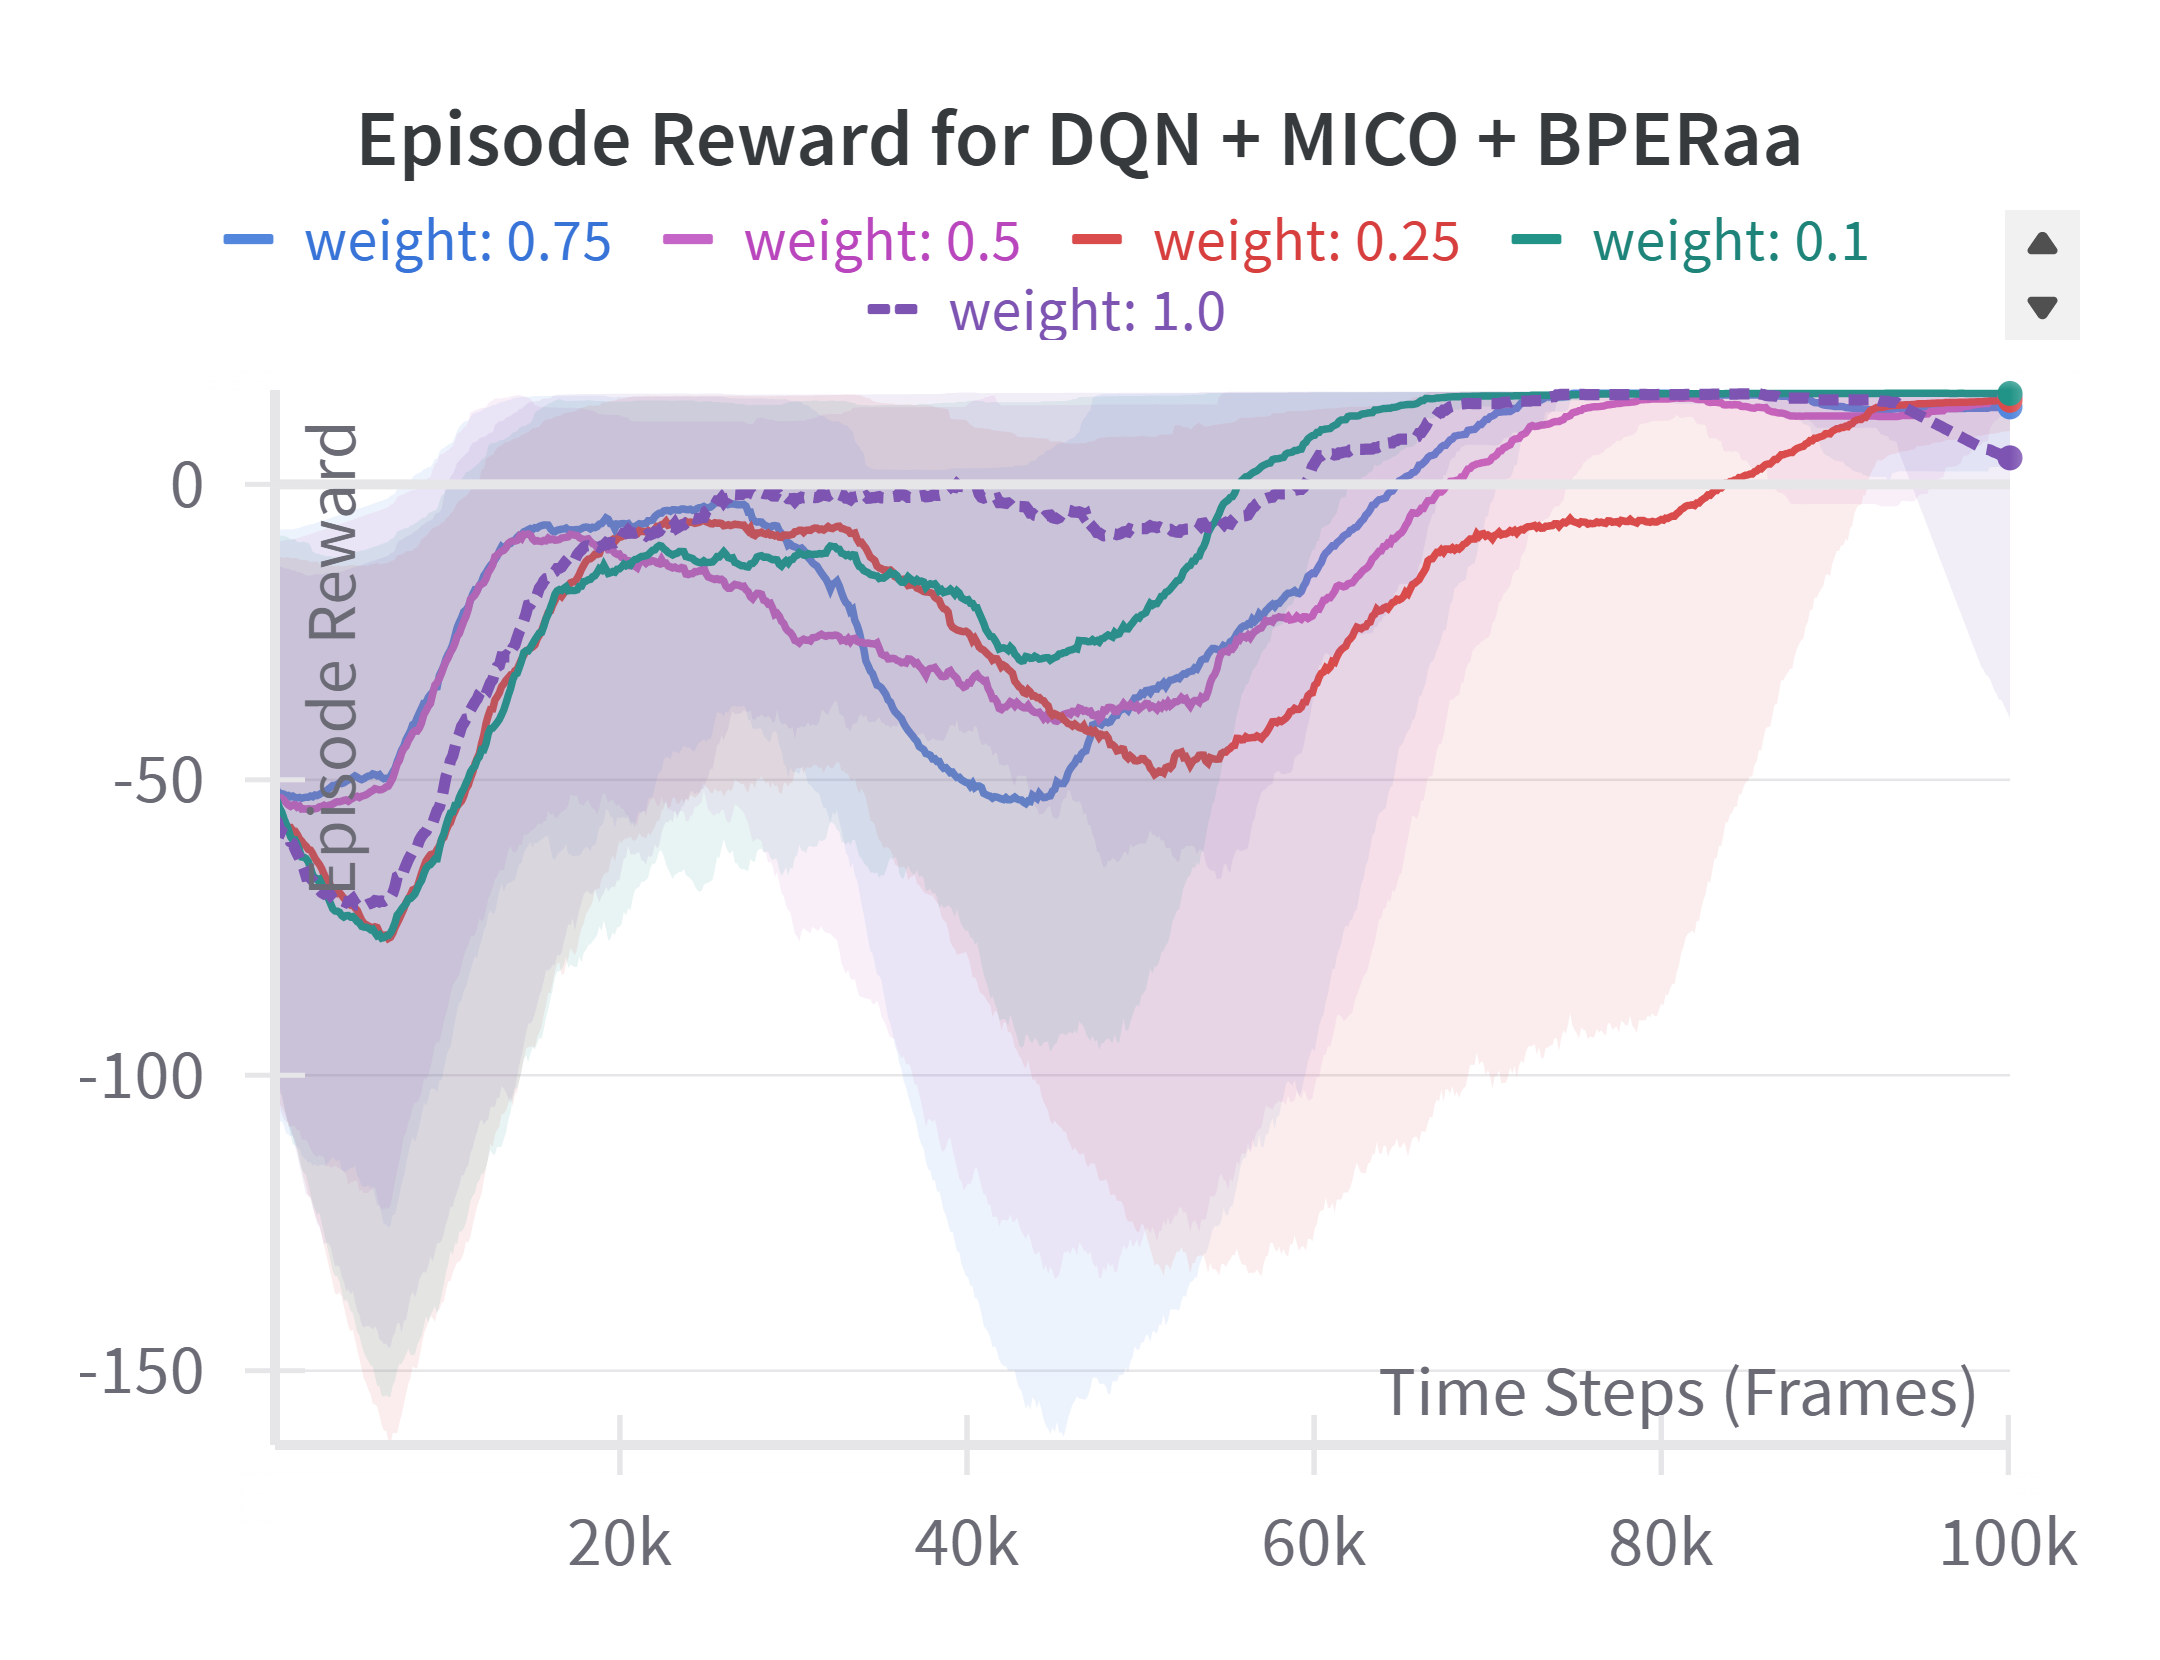
\includegraphics[width=\linewidth]{Results/grid_world/sweep_bperaa_grid_world.png}
        \caption{Sweep BPERcn}
        \label{fig:sweep_bperaa_grid_world}
    \end{subfigure}
    \caption[Priority Weight Sweep in Grid World]{\textbf{Priority Weight Sweep in Grid World.} TODO}
    \label{fig:sweep_methods_grid_world}
\end{figure}

\section{Mountain Car and CartPole with Priority Weight 1.0}
\label{append:results_priority_weight_1_0}
\begin{figure}[H]
    \centering
    \begin{subfigure}{0.45\textwidth}
    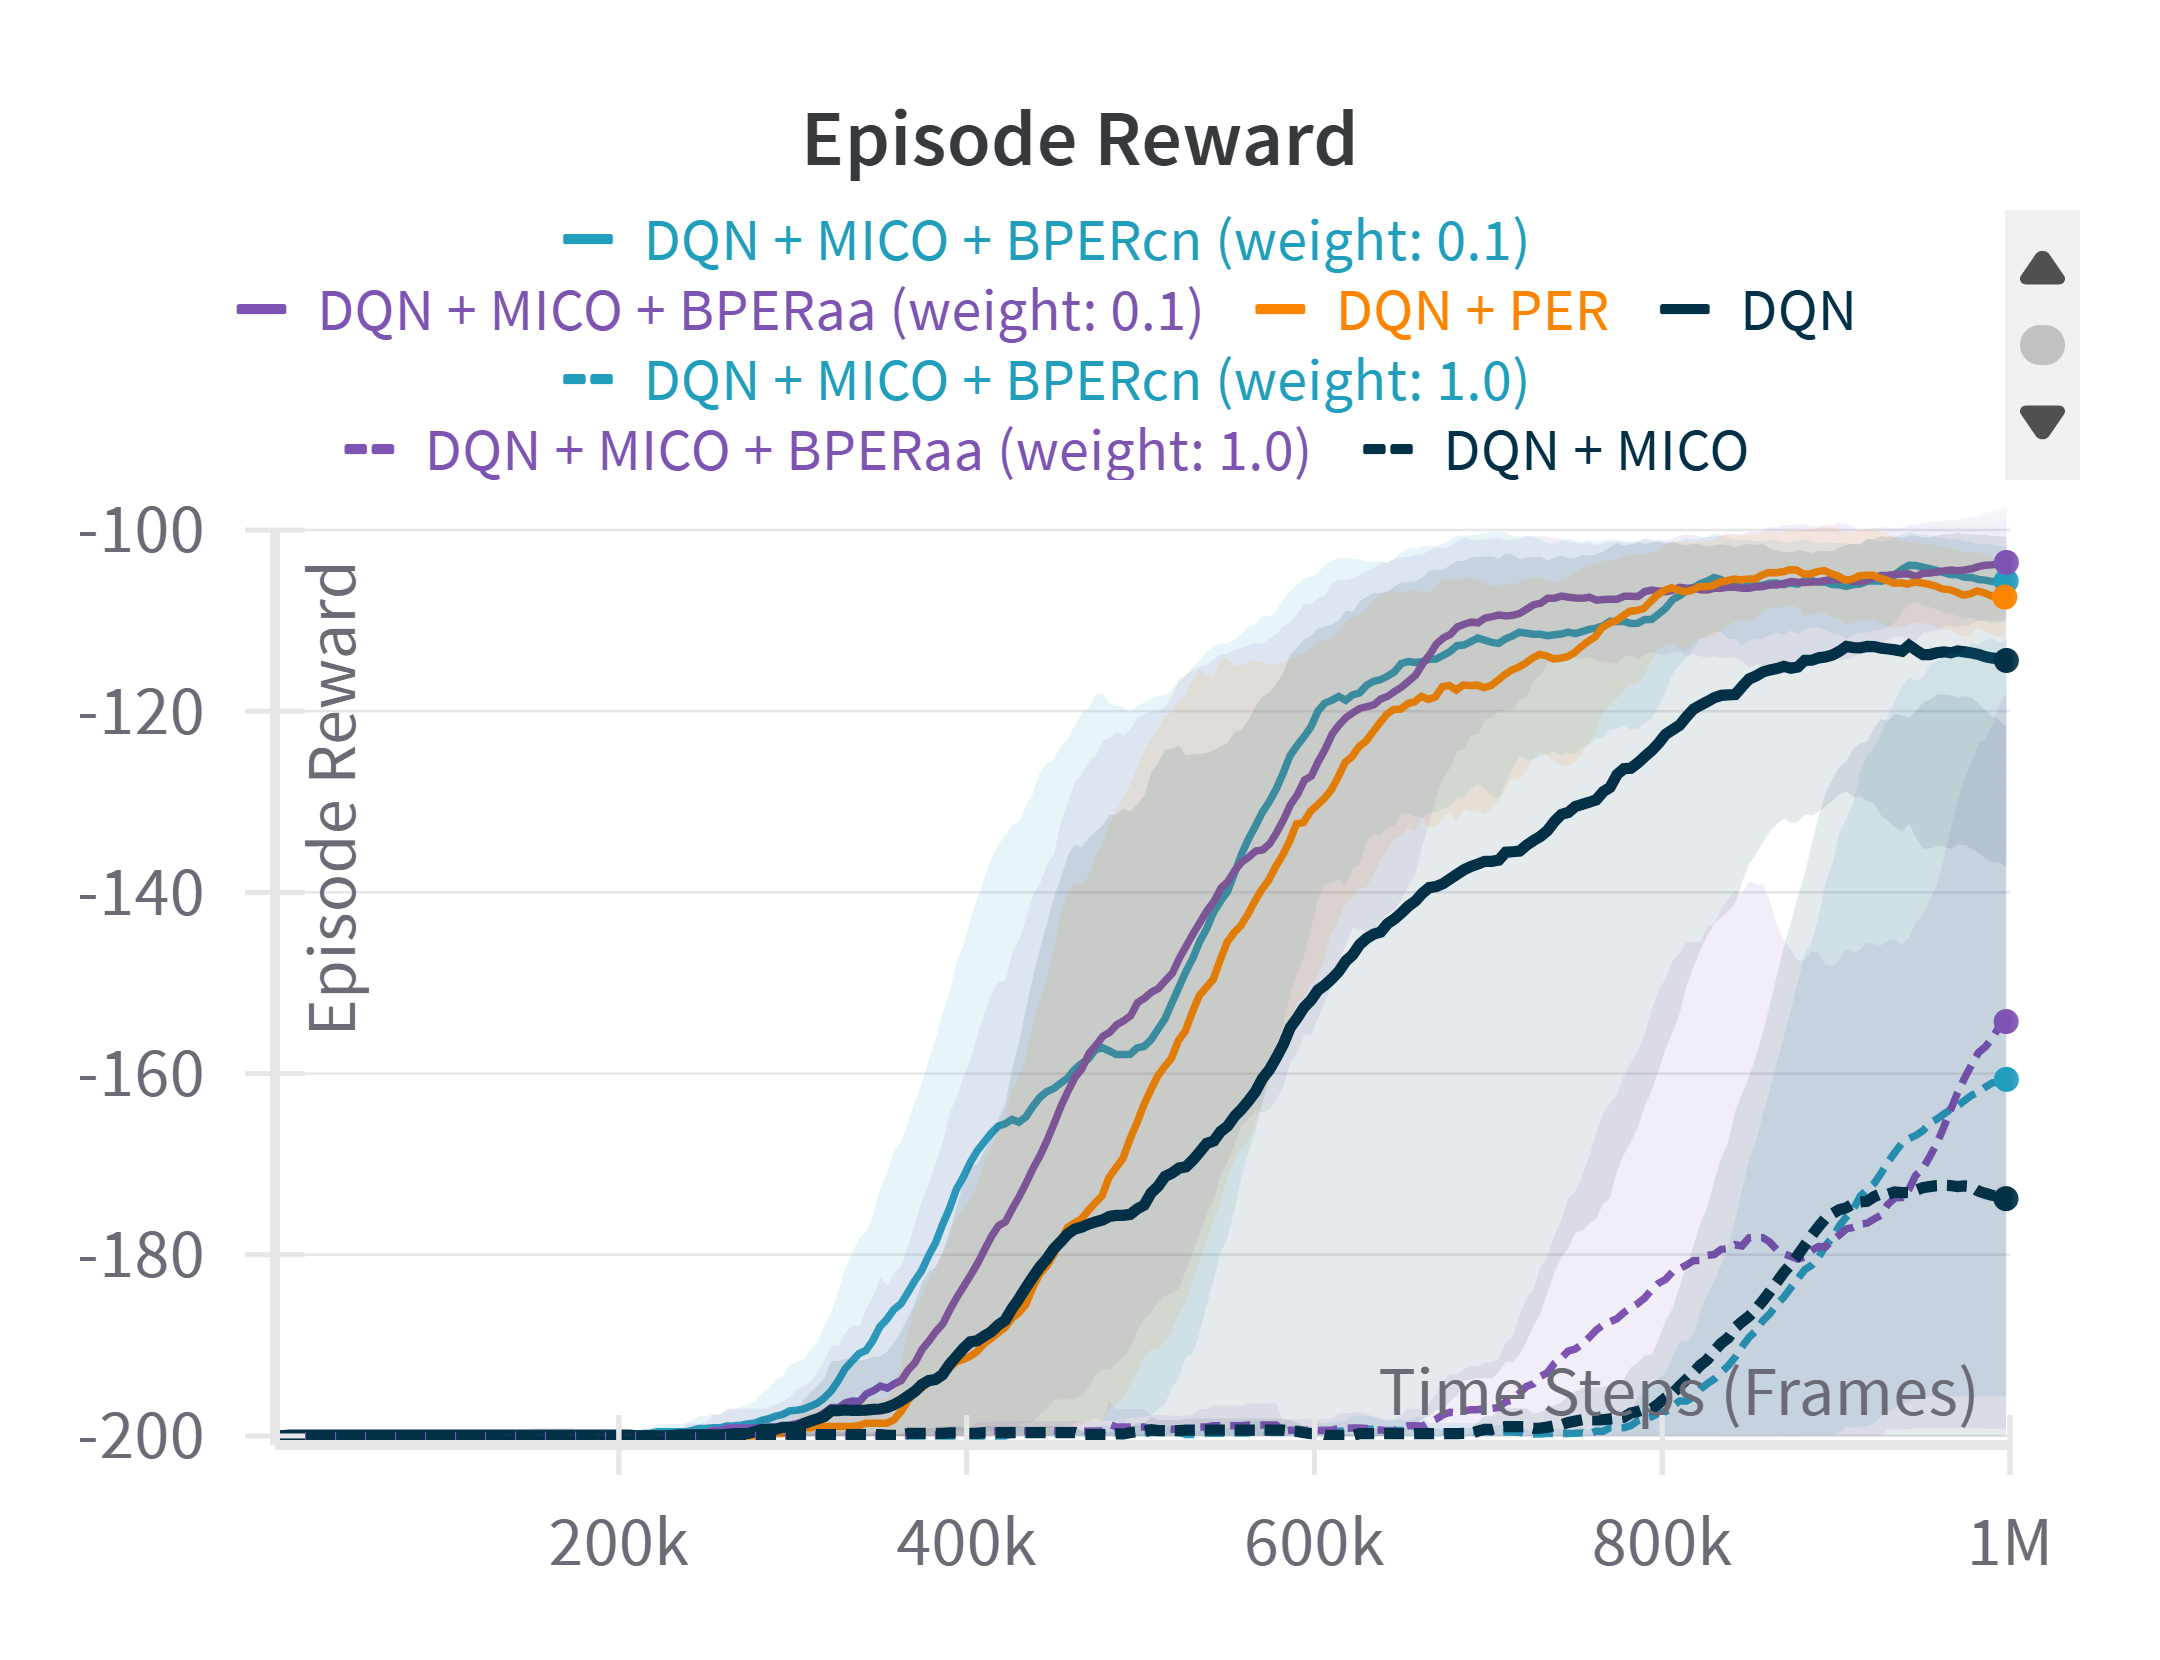
\includegraphics[width=\linewidth]{Results/general_results/return_mountain_car_weigh_1.png}
        \caption{Mountain Car}
        \label{fig:return_mountain_car_weigh_1}
    \end{subfigure}
    \hfill
    \begin{subfigure}{0.45\textwidth}
        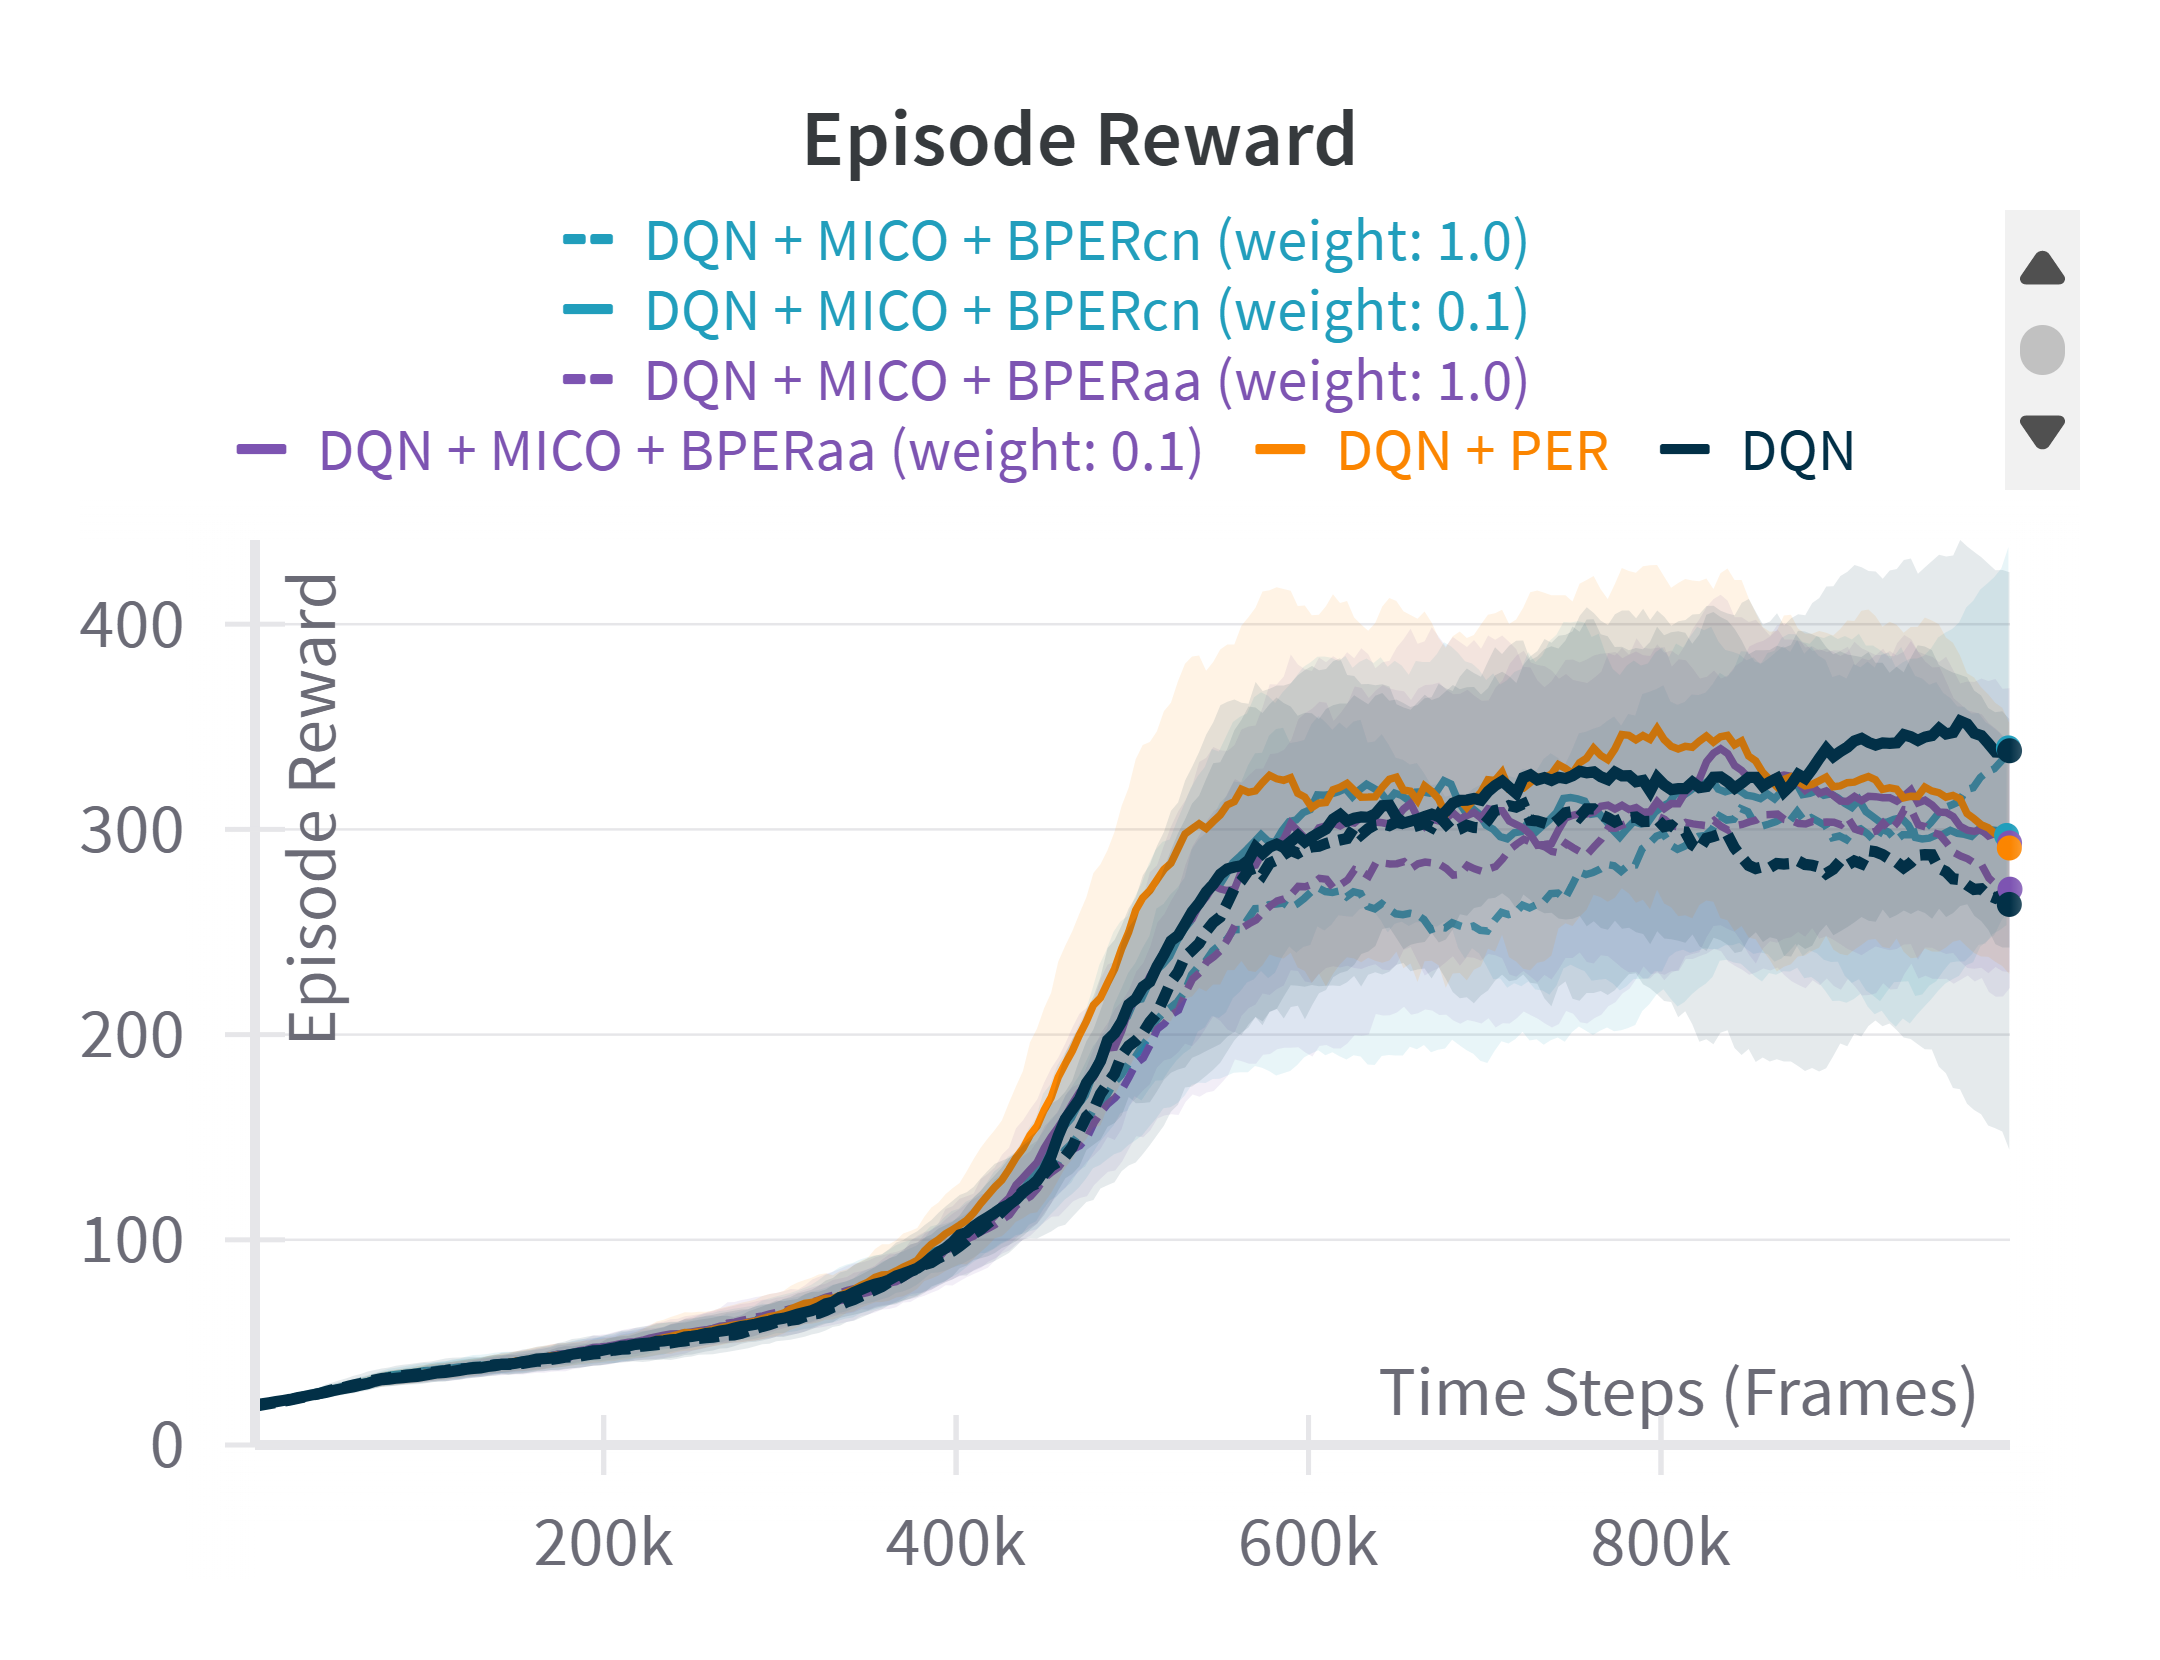
\includegraphics[width=\linewidth]{Results/general_results/return_cartpolev1_weight_1.png}
        \caption{CartPole}
        \label{fig:return_cartpolev1_weight_1}
    \end{subfigure}
    \caption[Episode Reward Priority Weight 1.0]{\textbf{Episode Reward Priority Weight 1.0.} TODO}
    \label{fig:return_methods_weight_1}
\end{figure}

\section{Visual Inspection 50k Time Step}
\label{append:visual_inspection_50k}

\begin{figure}[H]
    \centering
    \begin{subfigure}{1.\textwidth}
    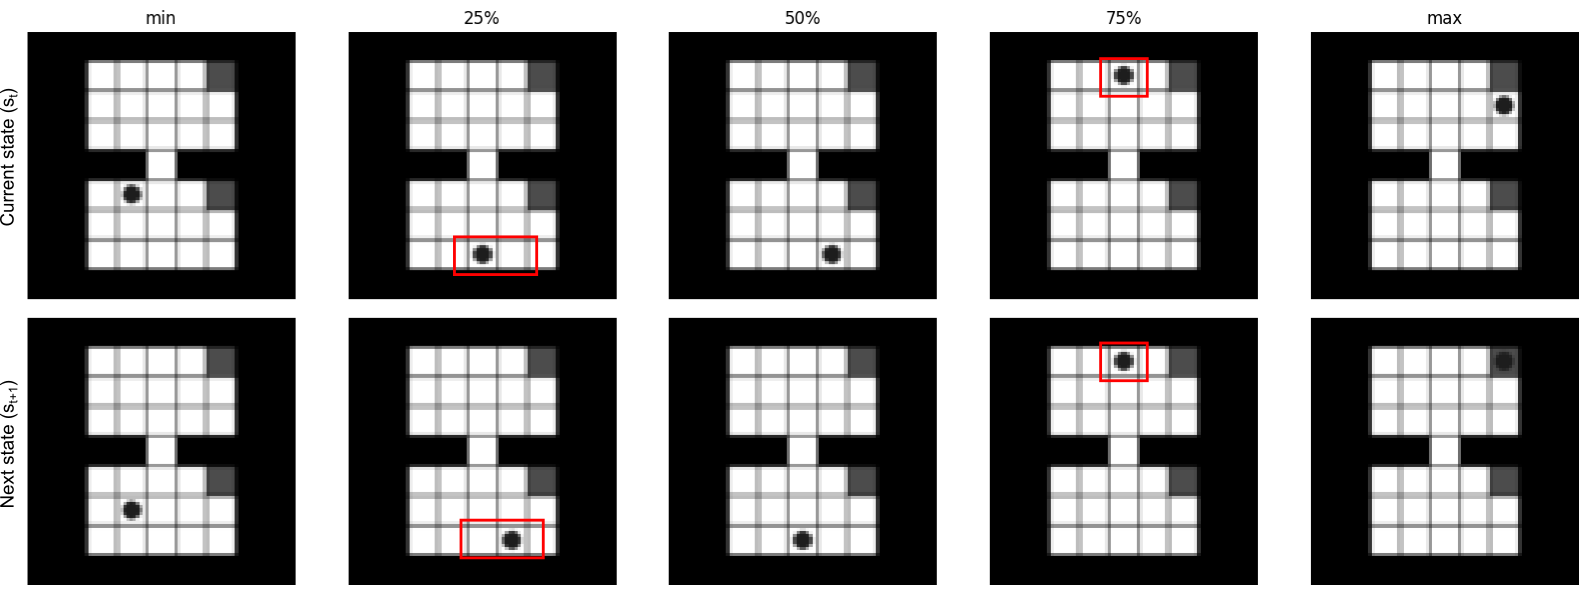
\includegraphics[width=\linewidth]{Results/grid_world/quartiles_images_per_50k.png}
        \caption{DQN + PER}
        \label{fig:quartiles_images_per_50k}
    \end{subfigure}
    \begin{subfigure}{1.\textwidth}
        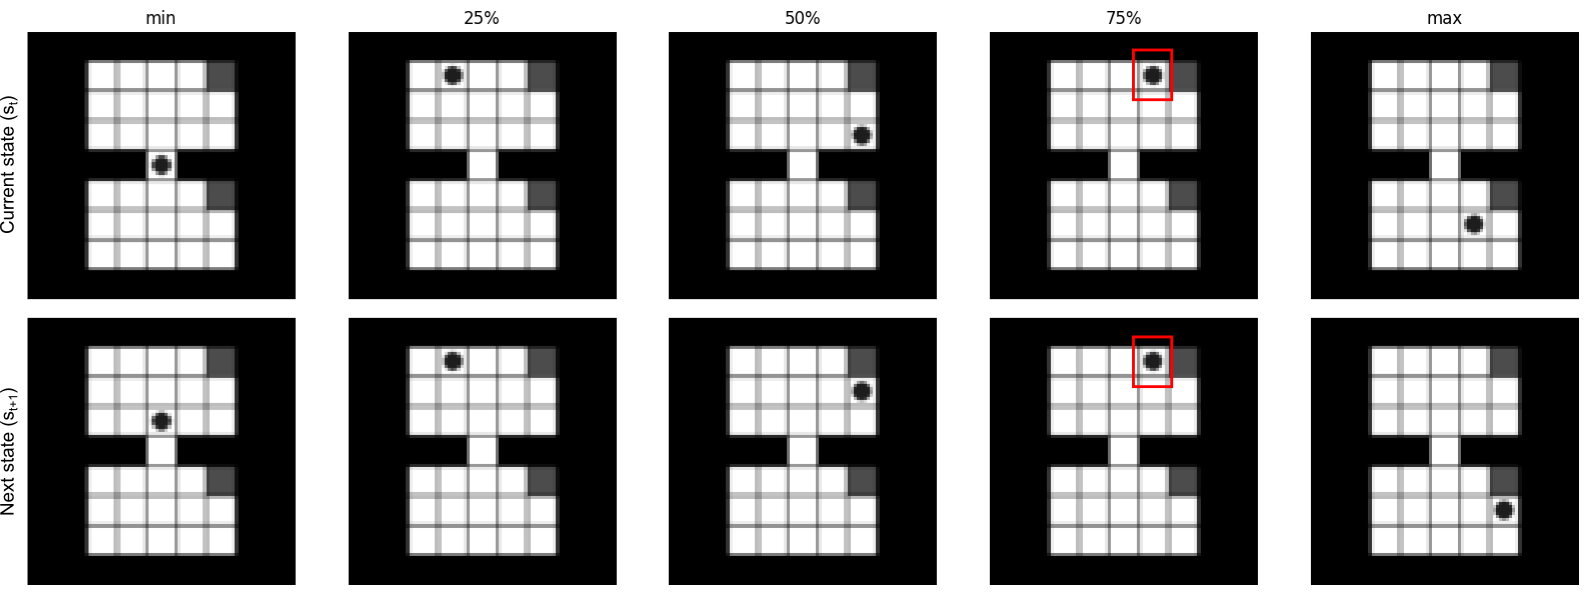
\includegraphics[width=\linewidth]{Results/grid_world/quartiles_images_dqn_mico_bpercn_50k.png}
        \caption{DQN (MICO) + BPERcn}
        \label{fig:quartiles_images_dqn_mico_bpercn_50k}
    \end{subfigure}
    \begin{subfigure}{1.\textwidth}
        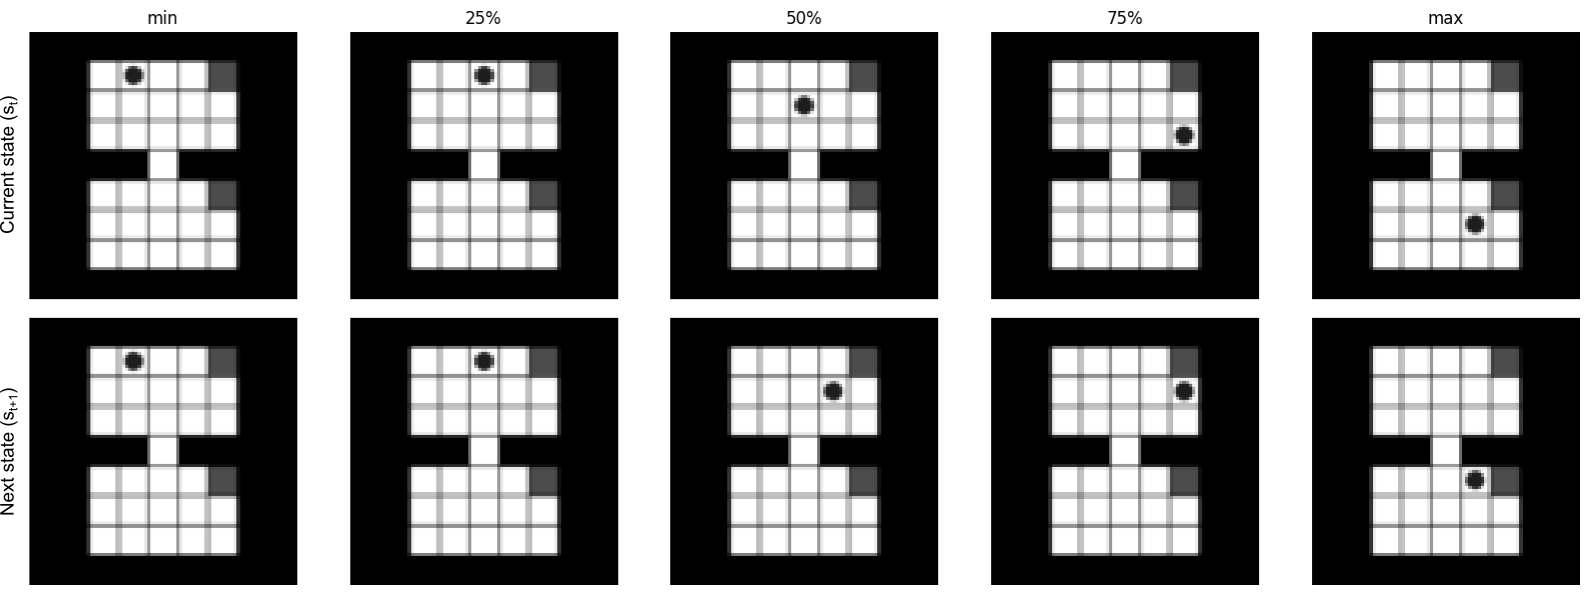
\includegraphics[width=\linewidth]{Results/grid_world/quartiles_images_dqn_mico_bperaa_50k.png}
        \caption{DQN (MICO) + BPERaa}
        \label{fig:quartiles_images_dqn_mico_bperaa_50k}
    \end{subfigure}
    \caption{Two images side-by-side}
    \label{fig:quartiles_all_methods_50k}
\end{figure}

\section{Episode Reward Gain baseline DQN + MICO}
\label{append:episode_reward_gain_dqn_mico}

\begin{figure}[h]
    \centering
    \begin{subfigure}{0.45\textwidth}
    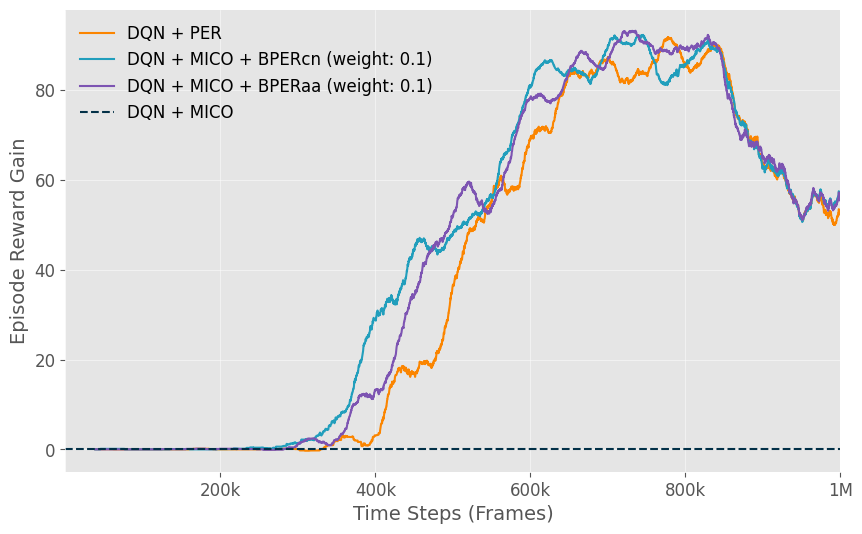
\includegraphics[width=\linewidth]{Results/general_results/mountain_car_reward_gain_vs_dqn_mico.png}
        \caption{MountainCar-v0}
        \label{fig:mountain_car_reward_gain_vs_dqn_mico}
    \end{subfigure}
    \hfill
    \begin{subfigure}{0.45\textwidth}
        \includegraphics[width=\linewidth]{Results/general_results/lunarlander_reward_gain_vs_dqn_mico.png}
        \caption{LunarLander-v1}
        \label{fig:lunarlander_reward_gain_vs_dqn_mico}
    \end{subfigure}
    \hfill
    \begin{subfigure}{0.45\textwidth}
        \includegraphics[width=\linewidth]{Results/general_results/cart_polev1_reward_gain_vs_dqn_mico.png}
        \caption{CartPole-v1}
        \label{fig:cart_polev1_reward_gain_vs_dqn_mico}
    \end{subfigure}
    \hfill
    \begin{subfigure}{0.45\textwidth}
        \includegraphics[width=\linewidth]{Results/general_results/acrobotv1_reward_gain_vs_dqn_mico.png}
        \caption{Acrobot-v1}
        \label{fig:acrobotv1_reward_gain_vs_dqn_mico}
    \end{subfigure}
    \caption{Two images side-by-side}
    \label{fig:reward_gain_vs_dqn_mico_methods}
\end{figure}

\section{Cumulative Reward for Lunar Lander}

\begin{figure}[H]
    \centering
    \includegraphics[width=1.\linewidth]{Results/general_results/cumulative_reward_lunar_lander.png}
    \caption[Cumulative Reward for Lunar Lander]{\textbf{Cumulative Reward for Lunar Lander}}
    \label{fig:cumulative_reward_lunar_lander}
\end{figure}

\section{Validation Results}




\end{document}
